\documentclass[conference]{IEEEtran}

% ============================================================
% Packages
% ============================================================
\usepackage{cite}
\usepackage{amsmath,amssymb,amsfonts}
\usepackage{algorithmic}
\usepackage{graphicx}
\usepackage{textcomp}
\usepackage{xcolor}
\usepackage{booktabs}
\usepackage{multirow}
\usepackage{hyperref}
\usepackage{array}
\usepackage{caption}
\usepackage{subcaption}
\usepackage{float}

\hypersetup{
    colorlinks=true,
    linkcolor=black,
    citecolor=blue,
    urlcolor=blue
}

\def\BibTeX{{\rm B\kern-.05em{\sc i\kern-.025em b}\kern-.08em
    T\kern-.1667em\lower.7ex\hbox{E}\kern-.125emX}}

\begin{document}

% ============================================================
% Title and Authors
% ============================================================
\title{Explainable Machine Learning for Air Quality Index Prediction in India: A Comparative Study of Regression, Classification, and Deep Learning Paradigms with SHAP-based Interpretability}

\author{
\IEEEauthorblockN{Samay Gada}
\IEEEauthorblockA{
Department of Computer Science \\
Mumbai, India \\
\textit{samaygada@example.com}}
}

\maketitle

% ============================================================
% ABSTRACT
% ============================================================
\begin{abstract}
Ambient air pollution poses a severe public health burden in India, where particulate matter concentrations routinely exceed World Health Organization guidelines by factors of five to ten. Accurate prediction of the Air Quality Index (AQI) enables timely public health interventions, yet existing studies typically evaluate a narrow set of models without post-hoc interpretability analysis. This paper presents a systematic comparison of 20 predictive models spanning three machine learning paradigms---regression, classification, and deep learning---applied to daily AQI data from 26 Indian cities over the period 2015--2020 (24,850 observations). A 141-feature representation was constructed from 12 raw pollutant measurements through temporal lag extraction, rolling window statistics, pollutant ratio computation, and seasonal encoding. For continuous AQI prediction, an Optuna-tuned LightGBM regressor achieved a coefficient of determination ($R^2$) of 0.9065 with a root mean squared error (RMSE) of 23.17 AQI units. For categorical AQI classification across six CPCB-defined severity levels, an XGBoost classifier attained 84.16\% accuracy, a macro $F_1$ score of 0.811, and a Cohen's $\kappa$ of 0.755 after SMOTE-based class balancing. Five deep learning architectures (LSTM, Stacked LSTM, Bidirectional LSTM, Conv1D-LSTM, GRU) yielded a maximum $R^2$ of 0.673, substantially underperforming gradient boosting methods by 23.4 percentage points. SHAP (SHapley Additive exPlanations) analysis on the best-performing models revealed that short-term PM\textsubscript{2.5} lag features and seasonal indicators are the dominant predictors, consistent with established atmospheric science. The held-out test set, which encompasses India's 2020 COVID-19 lockdown period, demonstrated that the models generalize to unprecedented reductions in anthropogenic emissions rather than memorizing temporal trends.
\end{abstract}

\begin{IEEEkeywords}
Air Quality Index, Machine Learning, LightGBM, XGBoost, LSTM, SHAP, Explainable AI, Feature Engineering, India, CPCB, Time Series Prediction, Gradient Boosting
\end{IEEEkeywords}

% ============================================================
% I. INTRODUCTION
% ============================================================
\section{Introduction}

\subsection{Problem Context and Motivation}

India bears a disproportionate share of the global air pollution burden. According to the World Health Organization (WHO), 14 of the 20 most polluted cities worldwide are located in India \cite{who2021}, and ambient particulate matter is estimated to contribute to over 1.67 million premature deaths annually in the country \cite{balakrishnan2019}. The Indo-Gangetic Plain, home to approximately 600 million people, regularly experiences winter-season PM\textsubscript{2.5} concentrations exceeding 300~$\mu$g/m$^3$---more than 20 times the WHO annual guideline of 15~$\mu$g/m$^3$ \cite{guttikunda2013}.

India's Central Pollution Control Board (CPCB) operationalises the National Air Quality Index, a single scalar metric derived from sub-indices of eight pollutant concentrations: PM\textsubscript{2.5}, PM\textsubscript{10}, NO\textsubscript{2}, SO\textsubscript{2}, CO, O\textsubscript{3}, NH\textsubscript{3}, and Pb \cite{cpcb2014}. The overall AQI equals the maximum sub-index across all measured pollutants, and the resulting value is classified into six severity categories: Good (0--50), Satisfactory (51--100), Moderate (101--200), Poor (201--300), Very Poor (301--400), and Severe (401--500). Accurate short-term AQI prediction is of direct practical value: it enables public health authorities to issue timely advisories, allows individuals with respiratory conditions to plan outdoor activities, and supports evidence-based policy interventions such as vehicular restrictions and industrial emission controls.

\subsection{Limitations of Existing Approaches}

A growing body of literature has applied machine learning techniques to AQI prediction in Indian cities \cite{kumar2022, sharma2020, masood2023}. However, several limitations persist in the existing work. First, most studies confine their evaluation to a single modelling paradigm---either regression or classification---without examining whether the same dataset supports different predictive formulations. Second, deep learning architectures such as Long Short-Term Memory (LSTM) networks are frequently adopted without a rigorous head-to-head comparison against well-tuned gradient boosting methods on identical preprocessed data, despite mounting evidence that tree-based models outperform neural networks on structured tabular datasets \cite{grinsztajn2022}. Third, the vast majority of published AQI models operate as opaque predictors: they report aggregate accuracy metrics without elucidating which features drive individual predictions. In a public health context, this lack of interpretability hinders trust, auditability, and actionable insight extraction. Finally, no prior study has explicitly evaluated model robustness under extreme distributional shift, such as the unprecedented reduction in anthropogenic emissions during India's COVID-19 lockdown (March--May 2020).

\subsection{Contributions}

This paper addresses the above gaps through the following contributions:

\begin{enumerate}
    \item A comprehensive comparison of 20 predictive models across three paradigms---eight regression models, seven classification models, and five deep learning architectures---trained and evaluated on an identically preprocessed dataset of 24,850 daily AQI observations from 26 Indian cities.
    \item A systematic feature engineering pipeline that transforms 12 raw pollutant measurements into a 141-dimensional representation incorporating temporal lags (1--30 days), rolling window statistics (3--30 days), pollutant concentration ratios, and India-specific seasonal encodings.
    \item Bayesian hyperparameter optimisation using Optuna with 50 Tree-structured Parzen Estimator (TPE) trials for the top-performing regression models, quantifying the marginal improvement over default configurations.
    \item A thorough post-hoc explainability analysis using SHAP (SHapley Additive exPlanations), including global feature importance, beeswarm interaction plots, non-linear dependence curves, and per-class explanations for the classification model.
    \item An empirical evaluation of model generalisation under distributional shift, with the held-out test set (February--July 2020) spanning India's national COVID-19 lockdown---a period characterised by 40--60\% reductions in vehicular and industrial emissions \cite{mahato2020}.
\end{enumerate}

\subsection{Paper Organisation}

The remainder of this paper is structured as follows. Section~II surveys related work on AQI prediction, deep learning for air quality, and explainable AI in environmental modelling. Section~III describes the dataset, preprocessing, and feature engineering pipeline. Section~IV details the modelling methodology, including regression, classification, deep learning architectures, hyperparameter optimisation, and the SHAP explainability framework. Section~V presents experimental results across all three paradigms. Section~VI provides the SHAP-based explainability analysis. Section~VII discusses key findings, the COVID-19 natural experiment, and study limitations. Section~VIII concludes the paper and outlines future research directions.

% ============================================================
% II. RELATED WORK
% ============================================================
\section{Related Work}

\subsection{Traditional and Ensemble Machine Learning for AQI Prediction}

Statistical and machine learning methods have been applied to air quality forecasting for over two decades. Early approaches relied on multiple linear regression and autoregressive integrated moving average (ARIMA) models, which capture linear pollutant--AQI relationships but fail to model the non-linear interactions between meteorological conditions and emission sources \cite{hastie2009}. Kumar and Pande \cite{kumar2022} applied random forests and gradient boosting to predict AQI across five Indian cities, reporting $R^2$ values between 0.78 and 0.85; however, their study was limited to three models and did not include hyperparameter tuning or interpretability analysis. Castelli \textit{et al.} \cite{castelli2020} employed genetic programming and support vector regression (SVR) for PM\textsubscript{2.5} prediction in California, achieving competitive results with SVR under radial basis function kernels but noting high sensitivity to kernel hyperparameters. Sharma \textit{et al.} \cite{sharma2020} proposed a hybrid framework combining empirical mode decomposition with extreme learning machines for hourly air quality forecasting, reporting mean absolute percentage errors below 15\% on single-station data. These studies collectively establish that ensemble tree-based methods and kernel machines can model pollutant dynamics effectively, but none undertake a systematic multi-paradigm comparison on a standardised Indian dataset.

\subsection{Deep Learning for Air Quality Forecasting}

Recurrent neural network architectures, particularly LSTMs \cite{hochreiter1997} and their gated variants \cite{cho2014}, have been widely applied to air quality time series on the premise that their hidden state memory captures temporal dependencies without explicit lag feature construction. Li \textit{et al.} \cite{li2020} demonstrated that LSTM networks outperform conventional feed-forward networks for 24-hour PM\textsubscript{2.5} prediction in Beijing, attributing the advantage to the cell gate mechanism's ability to retain multi-day pollution event signatures. Pak \textit{et al.} \cite{pak2020} introduced a spatiotemporal deep learning model incorporating convolutional layers for spatial pattern extraction followed by LSTM layers for temporal modelling, achieving a 12\% improvement over standalone LSTMs. Soh \textit{et al.} \cite{soh2018} proposed an adaptive deep learning architecture that selects the most relevant spatial--temporal relations, reporting state-of-the-art results on Taiwanese monitoring station data.

Despite these encouraging results, the claim that deep learning universally outperforms classical methods on environmental time series has been challenged. Grinsztajn \textit{et al.} \cite{grinsztajn2022} conducted a large-scale benchmark across 45 tabular datasets and found that tree-based models (XGBoost, LightGBM, random forests) outperformed deep learning in the majority of cases, particularly when the number of training samples was below 50{,}000 and the feature dimensionality was moderate. Shwartz-Ziv and Armon \cite{shwartzziv2022} reached a similar conclusion, noting that the inductive biases of decision trees---axis-aligned splits, feature selection, and handling of heterogeneous feature types---are well-suited to the irregular, mixed-type features common in environmental monitoring data. Borisov \textit{et al.} \cite{borisov2022} provided a comprehensive survey of deep learning methods for tabular data, identifying that the performance gap between tree-based and neural approaches narrows only with very large datasets or when raw unstructured inputs (images, text) are present alongside tabular features.

\subsection{Explainable AI in Environmental Modelling}

The demand for model interpretability in environmental and public health applications has grown substantially, driven by regulatory requirements and the need for stakeholder trust. SHAP (SHapley Additive exPlanations), introduced by Lundberg and Lee \cite{lundberg2017}, provides a unified framework grounded in cooperative game theory for attributing model predictions to individual feature contributions. Unlike permutation-based importance measures, SHAP values satisfy three desirable axiomatic properties: local accuracy, missingness, and consistency. Lundberg \textit{et al.} \cite{lundberg2020} subsequently developed TreeExplainer, an exact polynomial-time algorithm for computing SHAP values for tree-ensemble models, making large-scale explainability analysis computationally tractable.

LIME (Local Interpretable Model-agnostic Explanations) \cite{ribeiro2016} offers an alternative approach based on local linear surrogate models but lacks the theoretical guarantees of Shapley values and can produce unstable explanations under perturbation. Molnar \cite{molnar2022} provides a comprehensive treatment of interpretable machine learning methods, noting that SHAP has become the de facto standard for post-hoc explanation of tree-based models. In the air quality domain, SHAP has been applied to identify the relative contribution of meteorological versus emission-related features \cite{masood2023}, but comprehensive SHAP analyses covering both regression and classification formulations of AQI prediction remain scarce.

\subsection{Handling Class Imbalance and Data Quality}

AQI datasets exhibit pronounced class imbalance: moderate-quality days are far more frequent than extreme events (Good or Severe), creating a bias toward majority-class predictions in standard classifiers. The Synthetic Minority Over-sampling Technique (SMOTE) \cite{chawla2002} addresses this by generating synthetic samples along line segments connecting minority-class instances in feature space. Alternative strategies include cost-sensitive learning through class weights and threshold-moving techniques. The relative effectiveness of SMOTE versus built-in class weighting for multi-class ordinal targets such as AQI categories has not been systematically compared.

Missing data is endemic to India's air quality monitoring infrastructure: sensor malfunctions, calibration gaps, and intermittent station operation produce missing rates of 7--62\% across pollutant channels \cite{cpcb2014}. Multi-stage imputation pipelines combining within-series interpolation with cross-feature KNN imputation \cite{troyanskaya2001} have been shown to preserve inter-pollutant correlation structures while filling temporal gaps.

% ============================================================
% III. DATASET AND PREPROCESSING
% ============================================================
\section{Dataset and Preprocessing}

\subsection{Data Source and Description}

The primary dataset comprises daily city-level air quality measurements published by the Central Pollution Control Board (CPCB) of India, obtained via the Kaggle repository ``Air Quality Data in India'' (Rohan Rao, 2020). The dataset spans the period January 1, 2015 to July 1, 2020, encompassing 29{,}531 daily observations across 26 Indian cities from geographically diverse regions: the Indo-Gangetic Plain (Delhi, Lucknow, Patna), the western coast (Mumbai, Kochi), southern India (Bengaluru, Chennai, Hyderabad), the northeast (Guwahati, Shillong, Aizawl), and central India (Bhopal, Ahmedabad).

Each record contains 12 pollutant concentrations measured in $\mu$g/m$^3$ (except CO in mg/m$^3$): PM\textsubscript{2.5}, PM\textsubscript{10}, NO, NO\textsubscript{2}, NO\textsubscript{x}, NH\textsubscript{3}, CO, SO\textsubscript{2}, O\textsubscript{3}, Benzene, Toluene, and Xylene. Two target variables are provided: a continuous AQI value and a categorical AQI\_Bucket with six severity levels. A second, ostensibly updated dataset covering 2015--2024 was evaluated during preliminary analysis but was rejected due to synthetic characteristics: near-zero pollutant--AQI correlations ($r < 0.05$), perfectly balanced category distributions, and negative $R^2$ scores across all regression models.

\subsection{Exploratory Data Analysis}

\begin{figure}[!t]
\centering
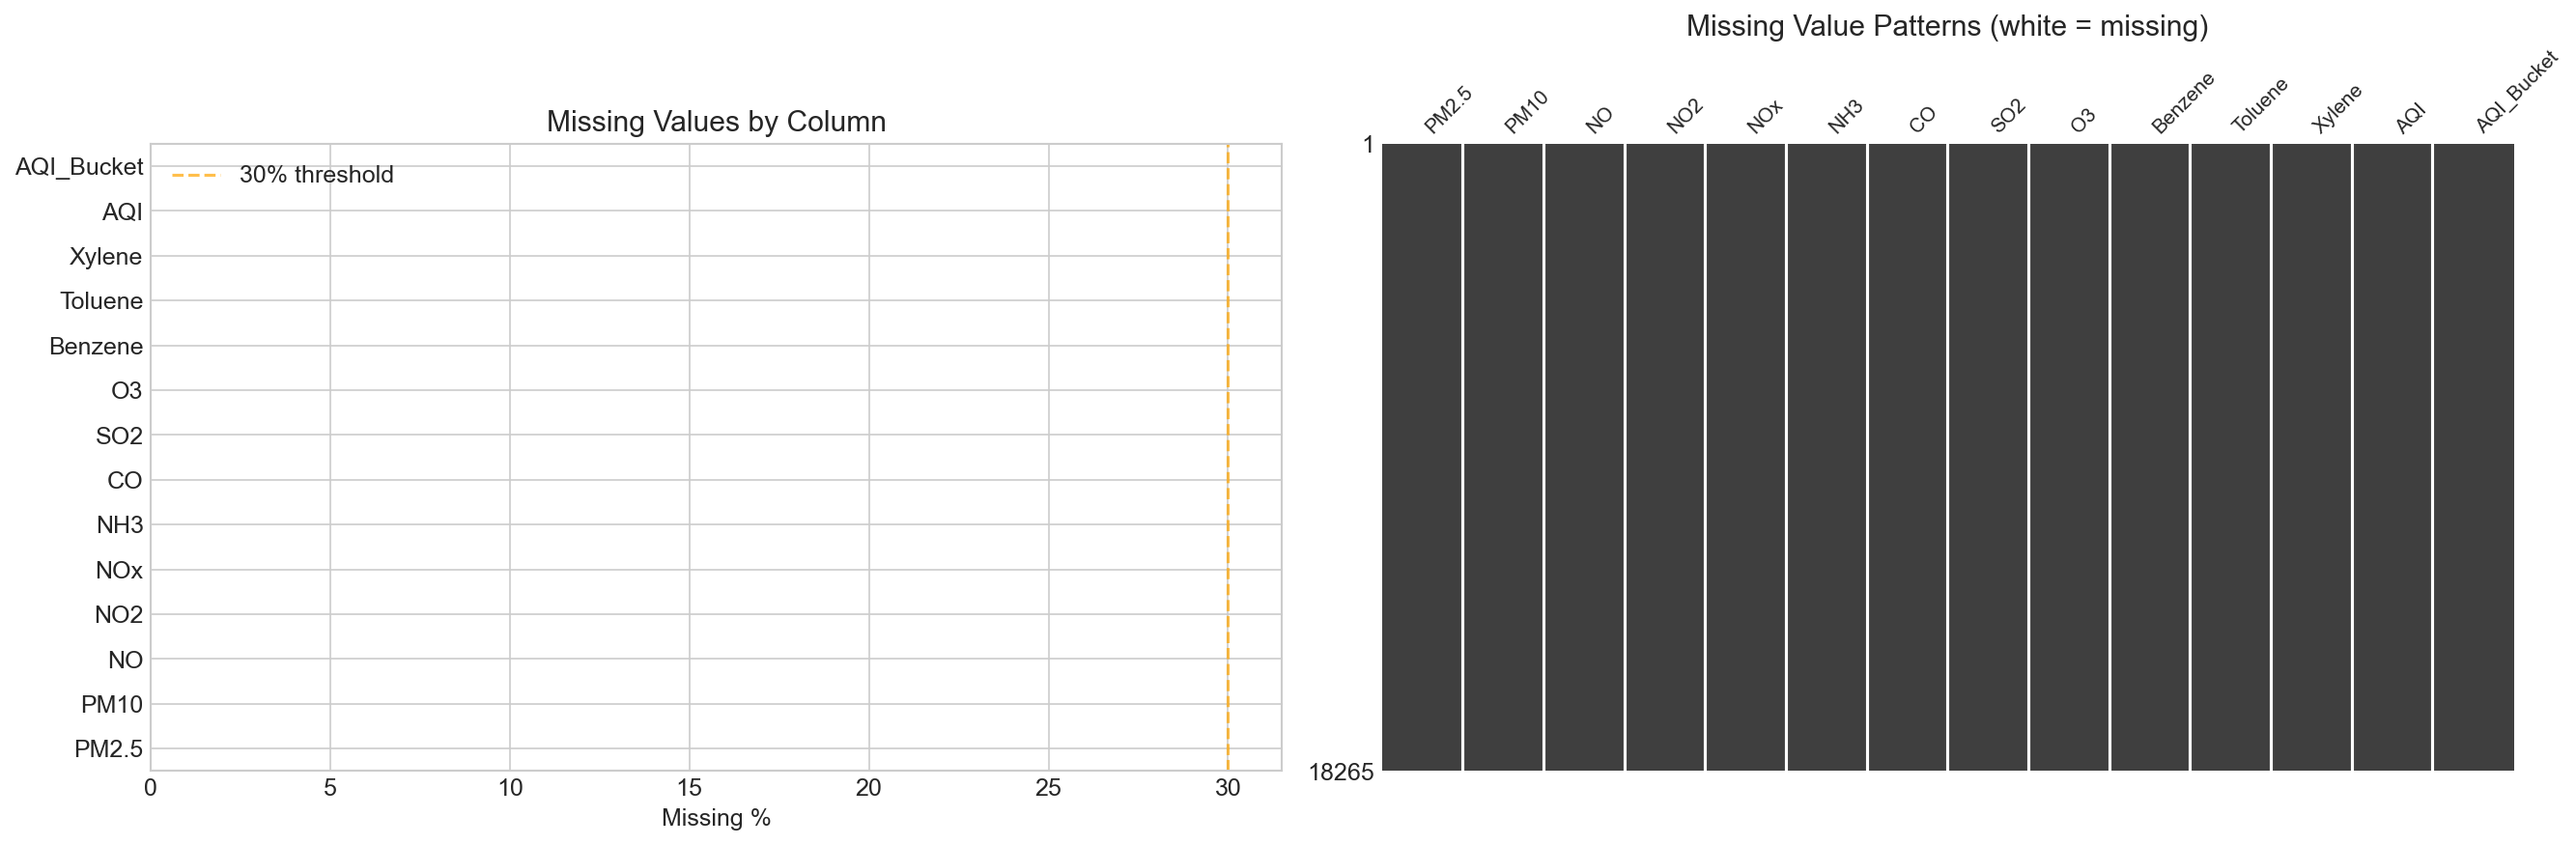
\includegraphics[width=\columnwidth]{figures/01_missing_values.png}
\caption{Missing value percentages across pollutant features. Xylene exhibits the highest missing rate (61.3\%), followed by PM\textsubscript{10} (37.7\%) and NH\textsubscript{3} (35.0\%). The AQI target variable is missing for 15.9\% of records.}
\label{fig:missing}
\end{figure}

Missing data is pervasive across the dataset, as shown in Fig.~\ref{fig:missing}. Missing rates range from 7.0\% (CO) to 61.3\% (Xylene), with a total of 88{,}488 missing cells across 29{,}531 rows. The missingness pattern is non-random: northeastern cities (Aizawl, Shillong) exhibit higher missing rates than major metropolitan centres, reflecting disparities in monitoring infrastructure.

\begin{figure}[!t]
\centering
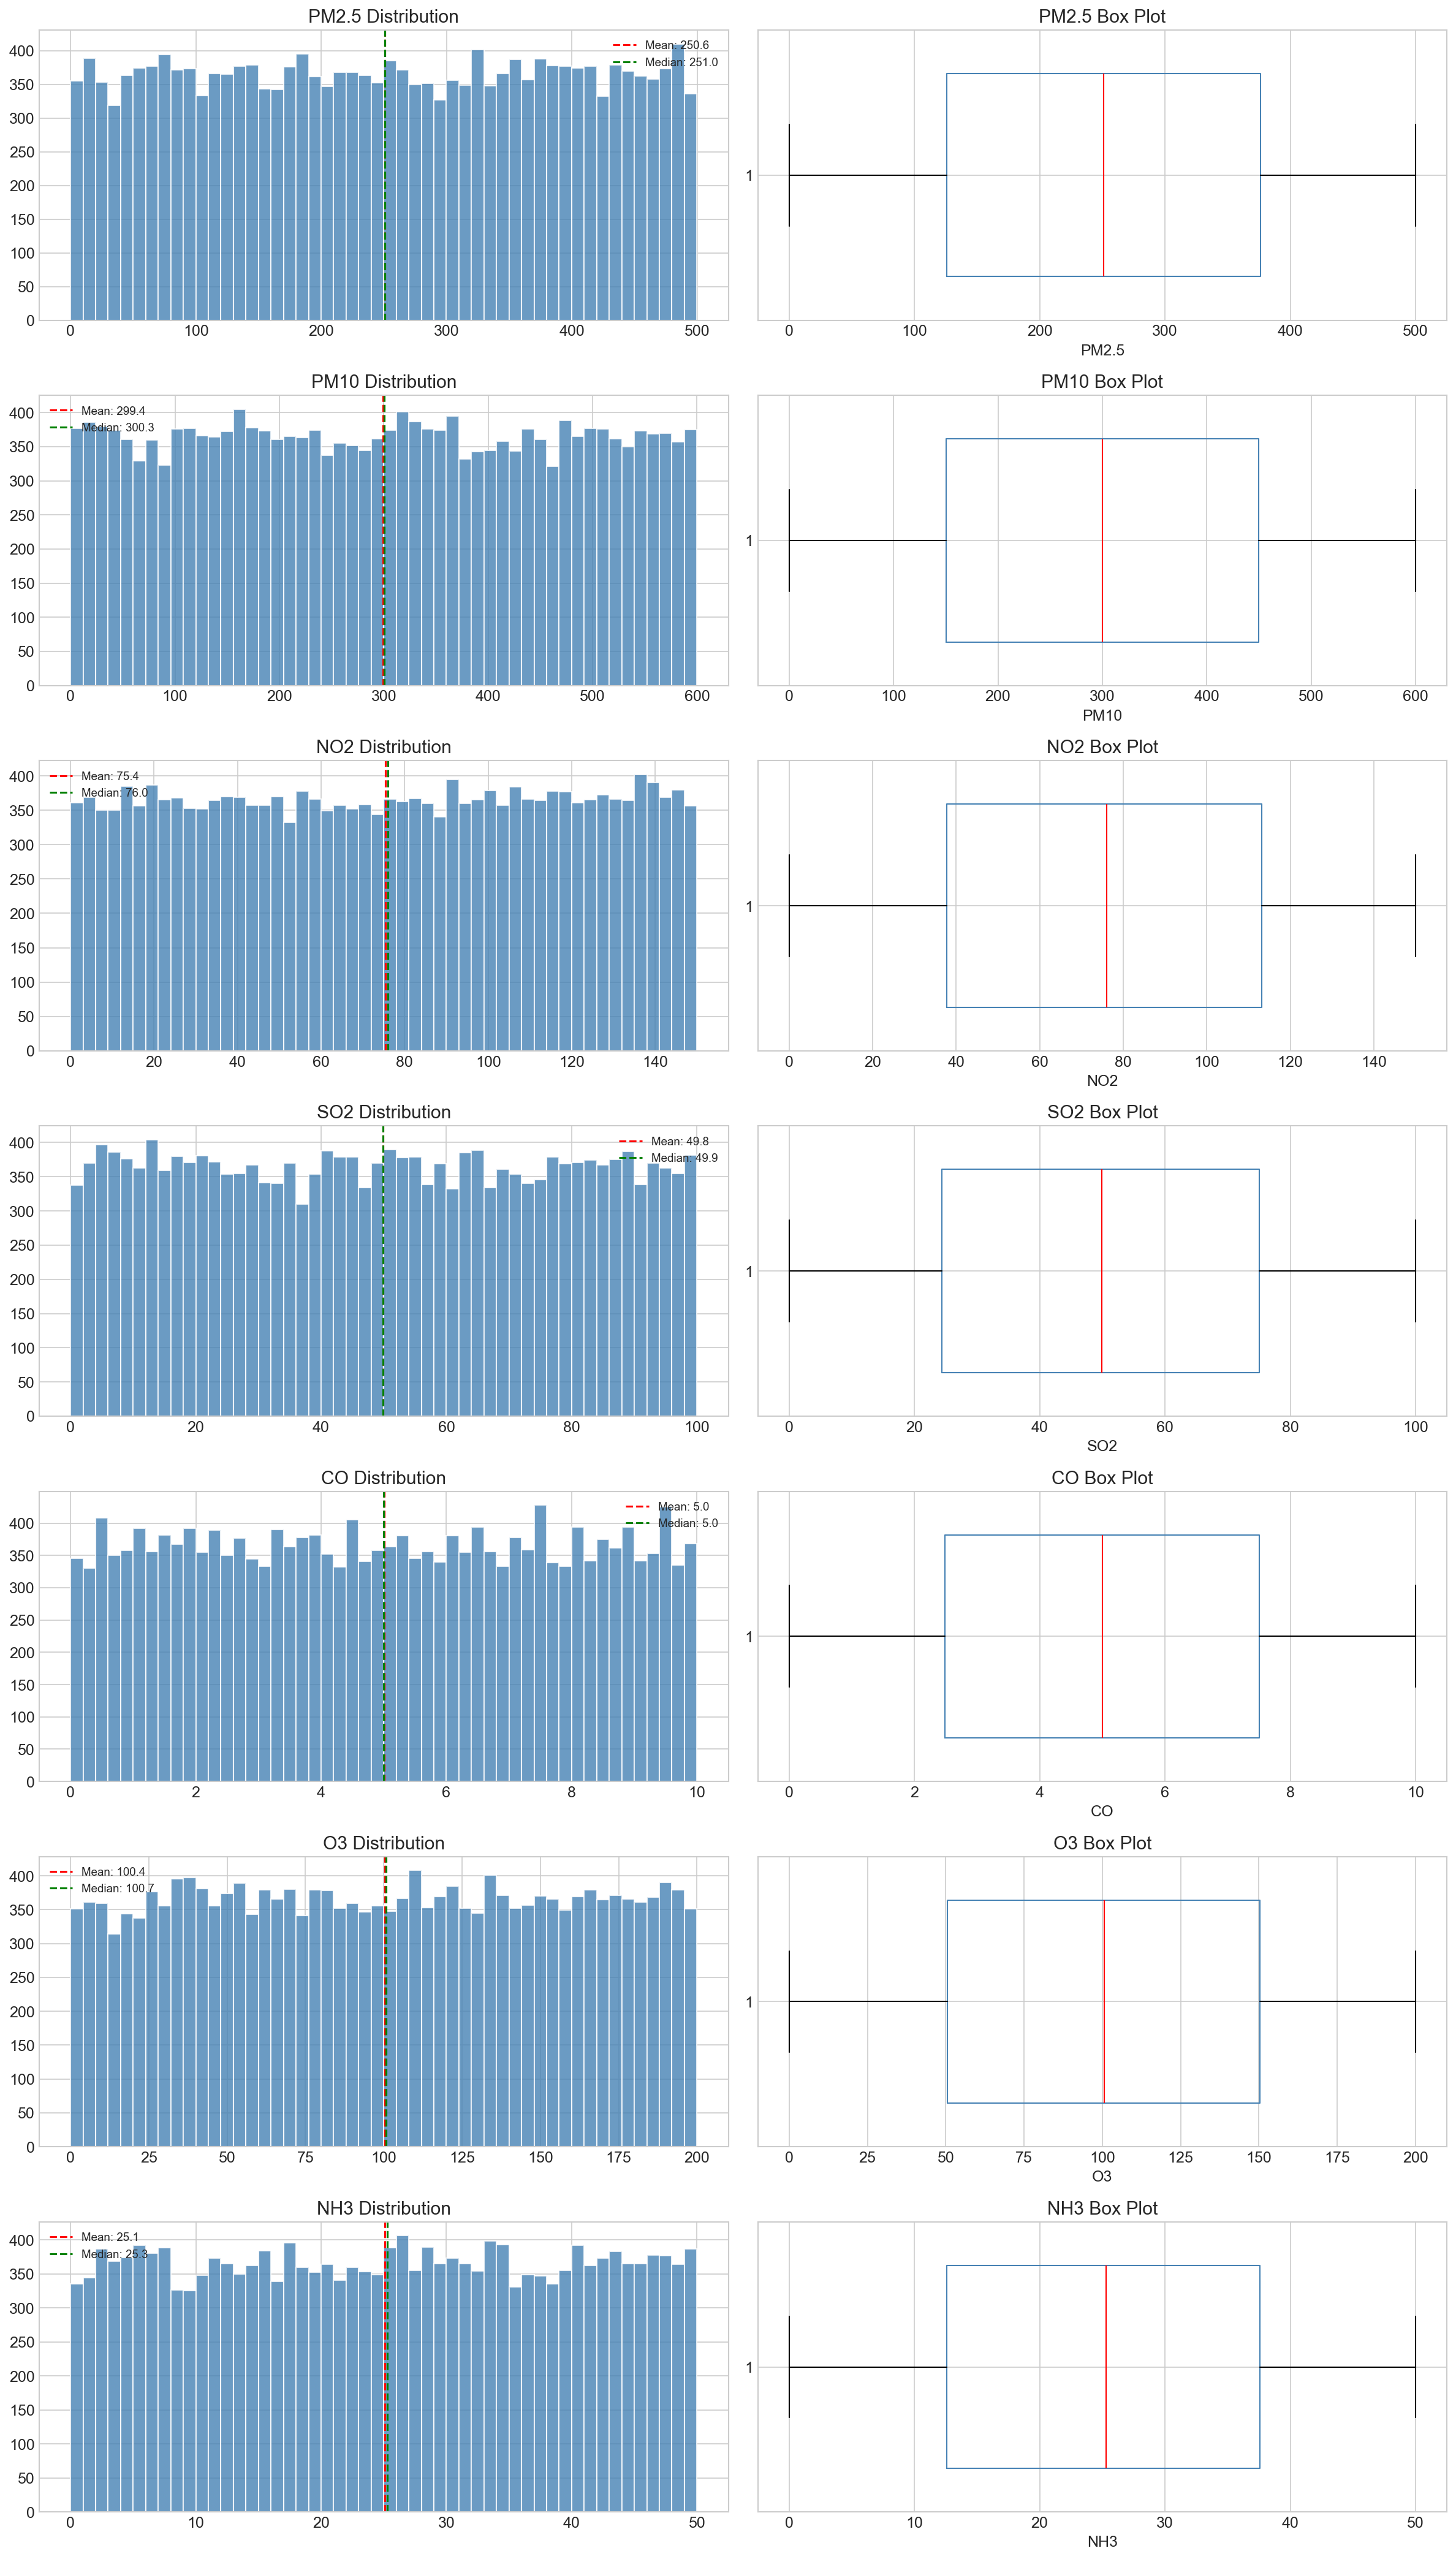
\includegraphics[width=\columnwidth]{figures/03_pollutant_distributions.png}
\caption{Distribution of pollutant concentrations and AQI values. Most pollutants exhibit pronounced right-skewness with long tails, indicating intermittent high-pollution events superimposed on a lower baseline.}
\label{fig:distributions}
\end{figure}

Pollutant distributions (Fig.~\ref{fig:distributions}) are uniformly right-skewed, consistent with the episodic nature of pollution events. PM\textsubscript{2.5} and PM\textsubscript{10} display the widest ranges and the strongest linear correlations with AQI (Pearson $r = 0.659$ and $r = 0.803$, respectively), confirming their role as dominant AQI determinants under the CPCB framework.

\begin{figure}[!t]
\centering
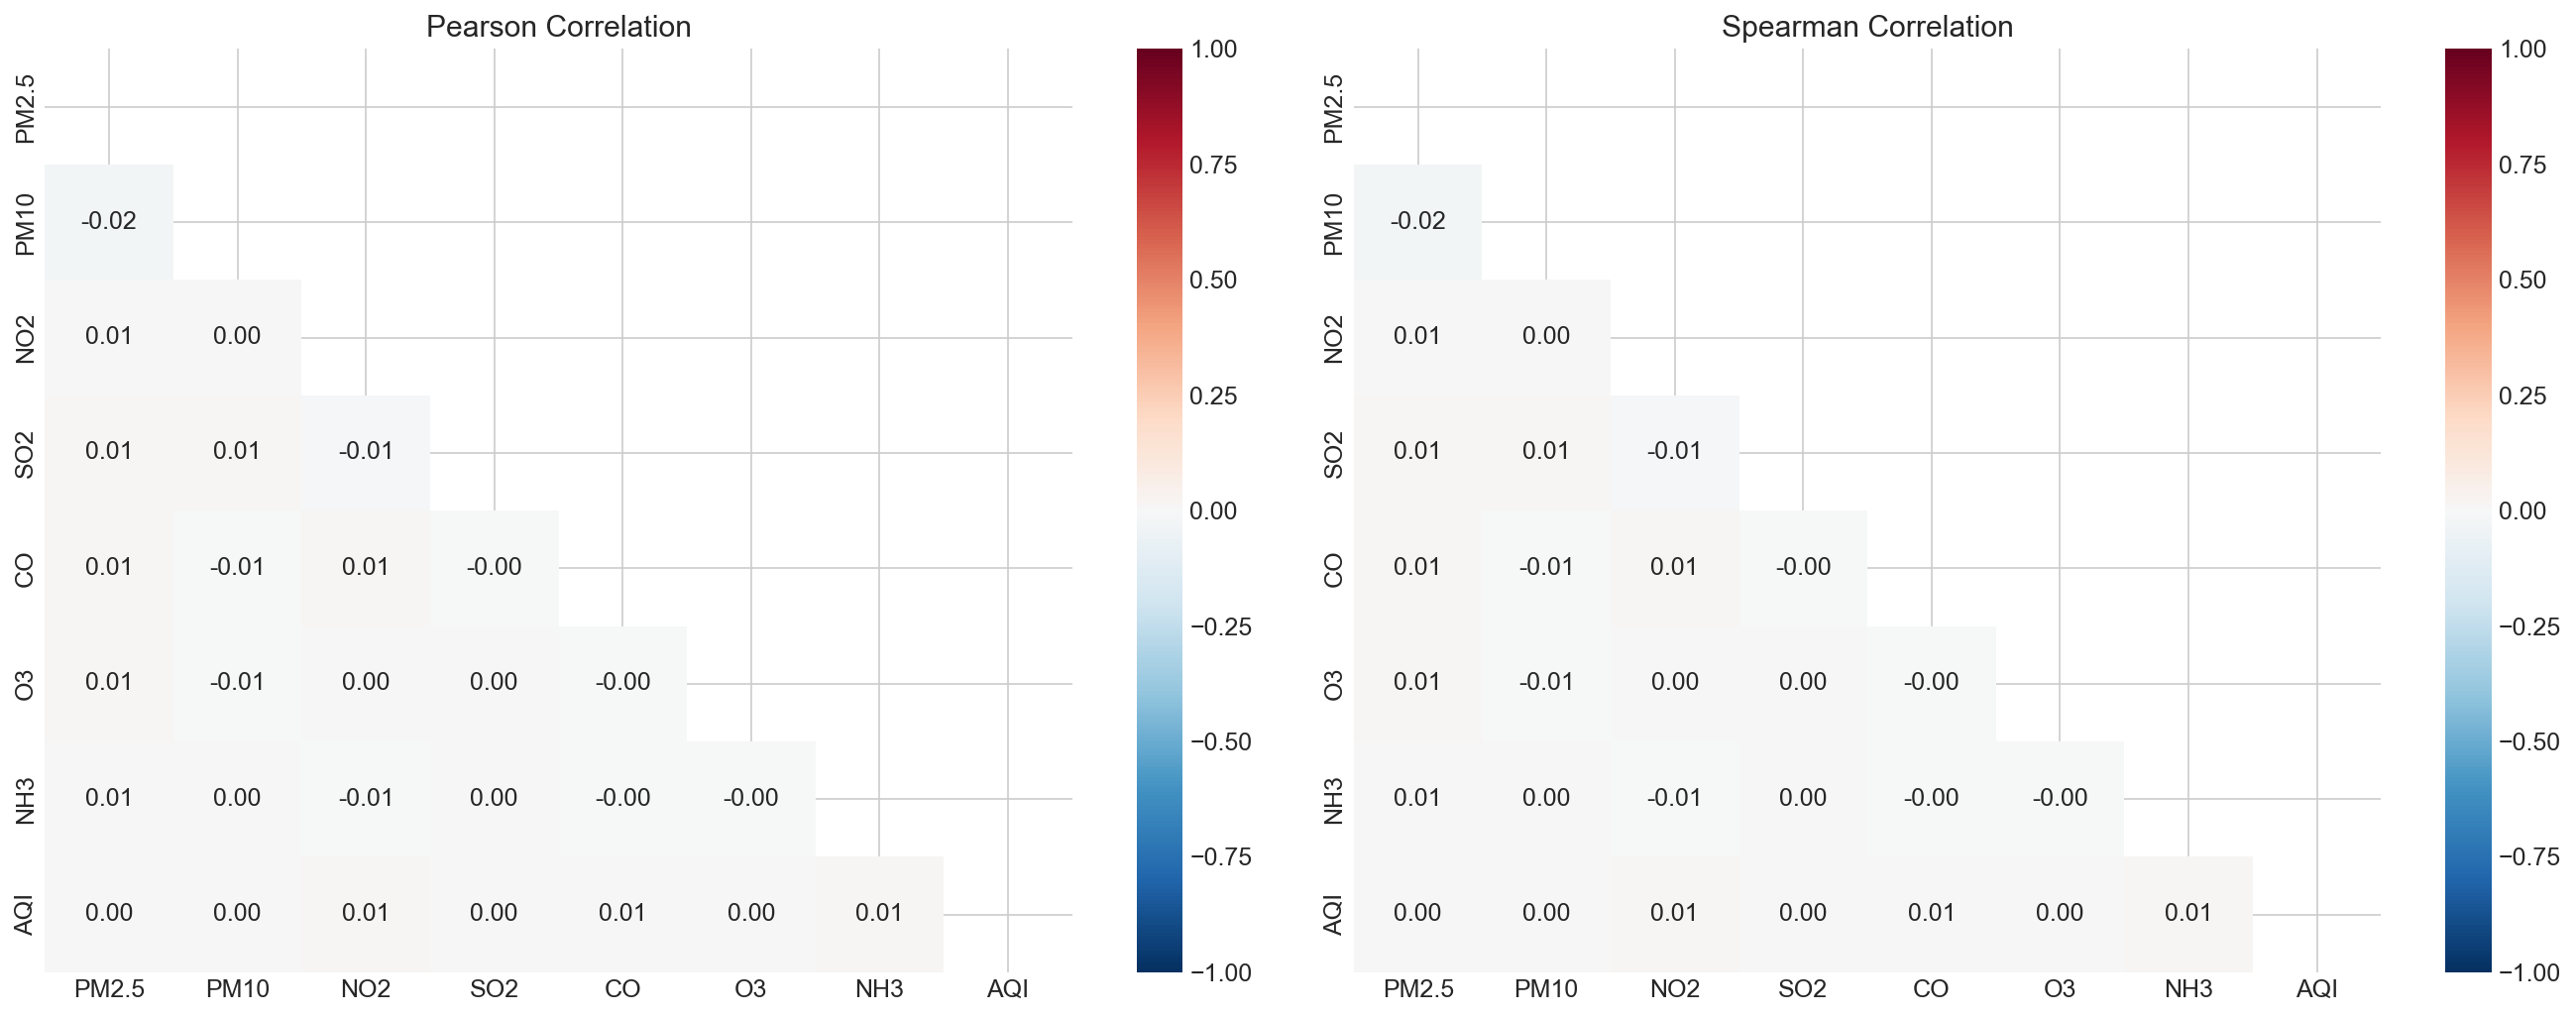
\includegraphics[width=\columnwidth]{figures/05_correlations.png}
\caption{Pearson and Spearman correlation matrices for pollutant features and AQI. PM\textsubscript{10} ($r = 0.803$) and CO ($r = 0.683$) exhibit the strongest linear associations with AQI.}
\label{fig:correlations}
\end{figure}

Correlation analysis (Fig.~\ref{fig:correlations}) reveals strong inter-pollutant dependencies: PM\textsubscript{2.5} and PM\textsubscript{10} are highly correlated ($r = 0.87$), as are NO\textsubscript{2} and NO\textsubscript{x} ($r = 0.93$), reflecting shared emission sources (vehicular combustion, construction dust).

\begin{figure}[!t]
\centering
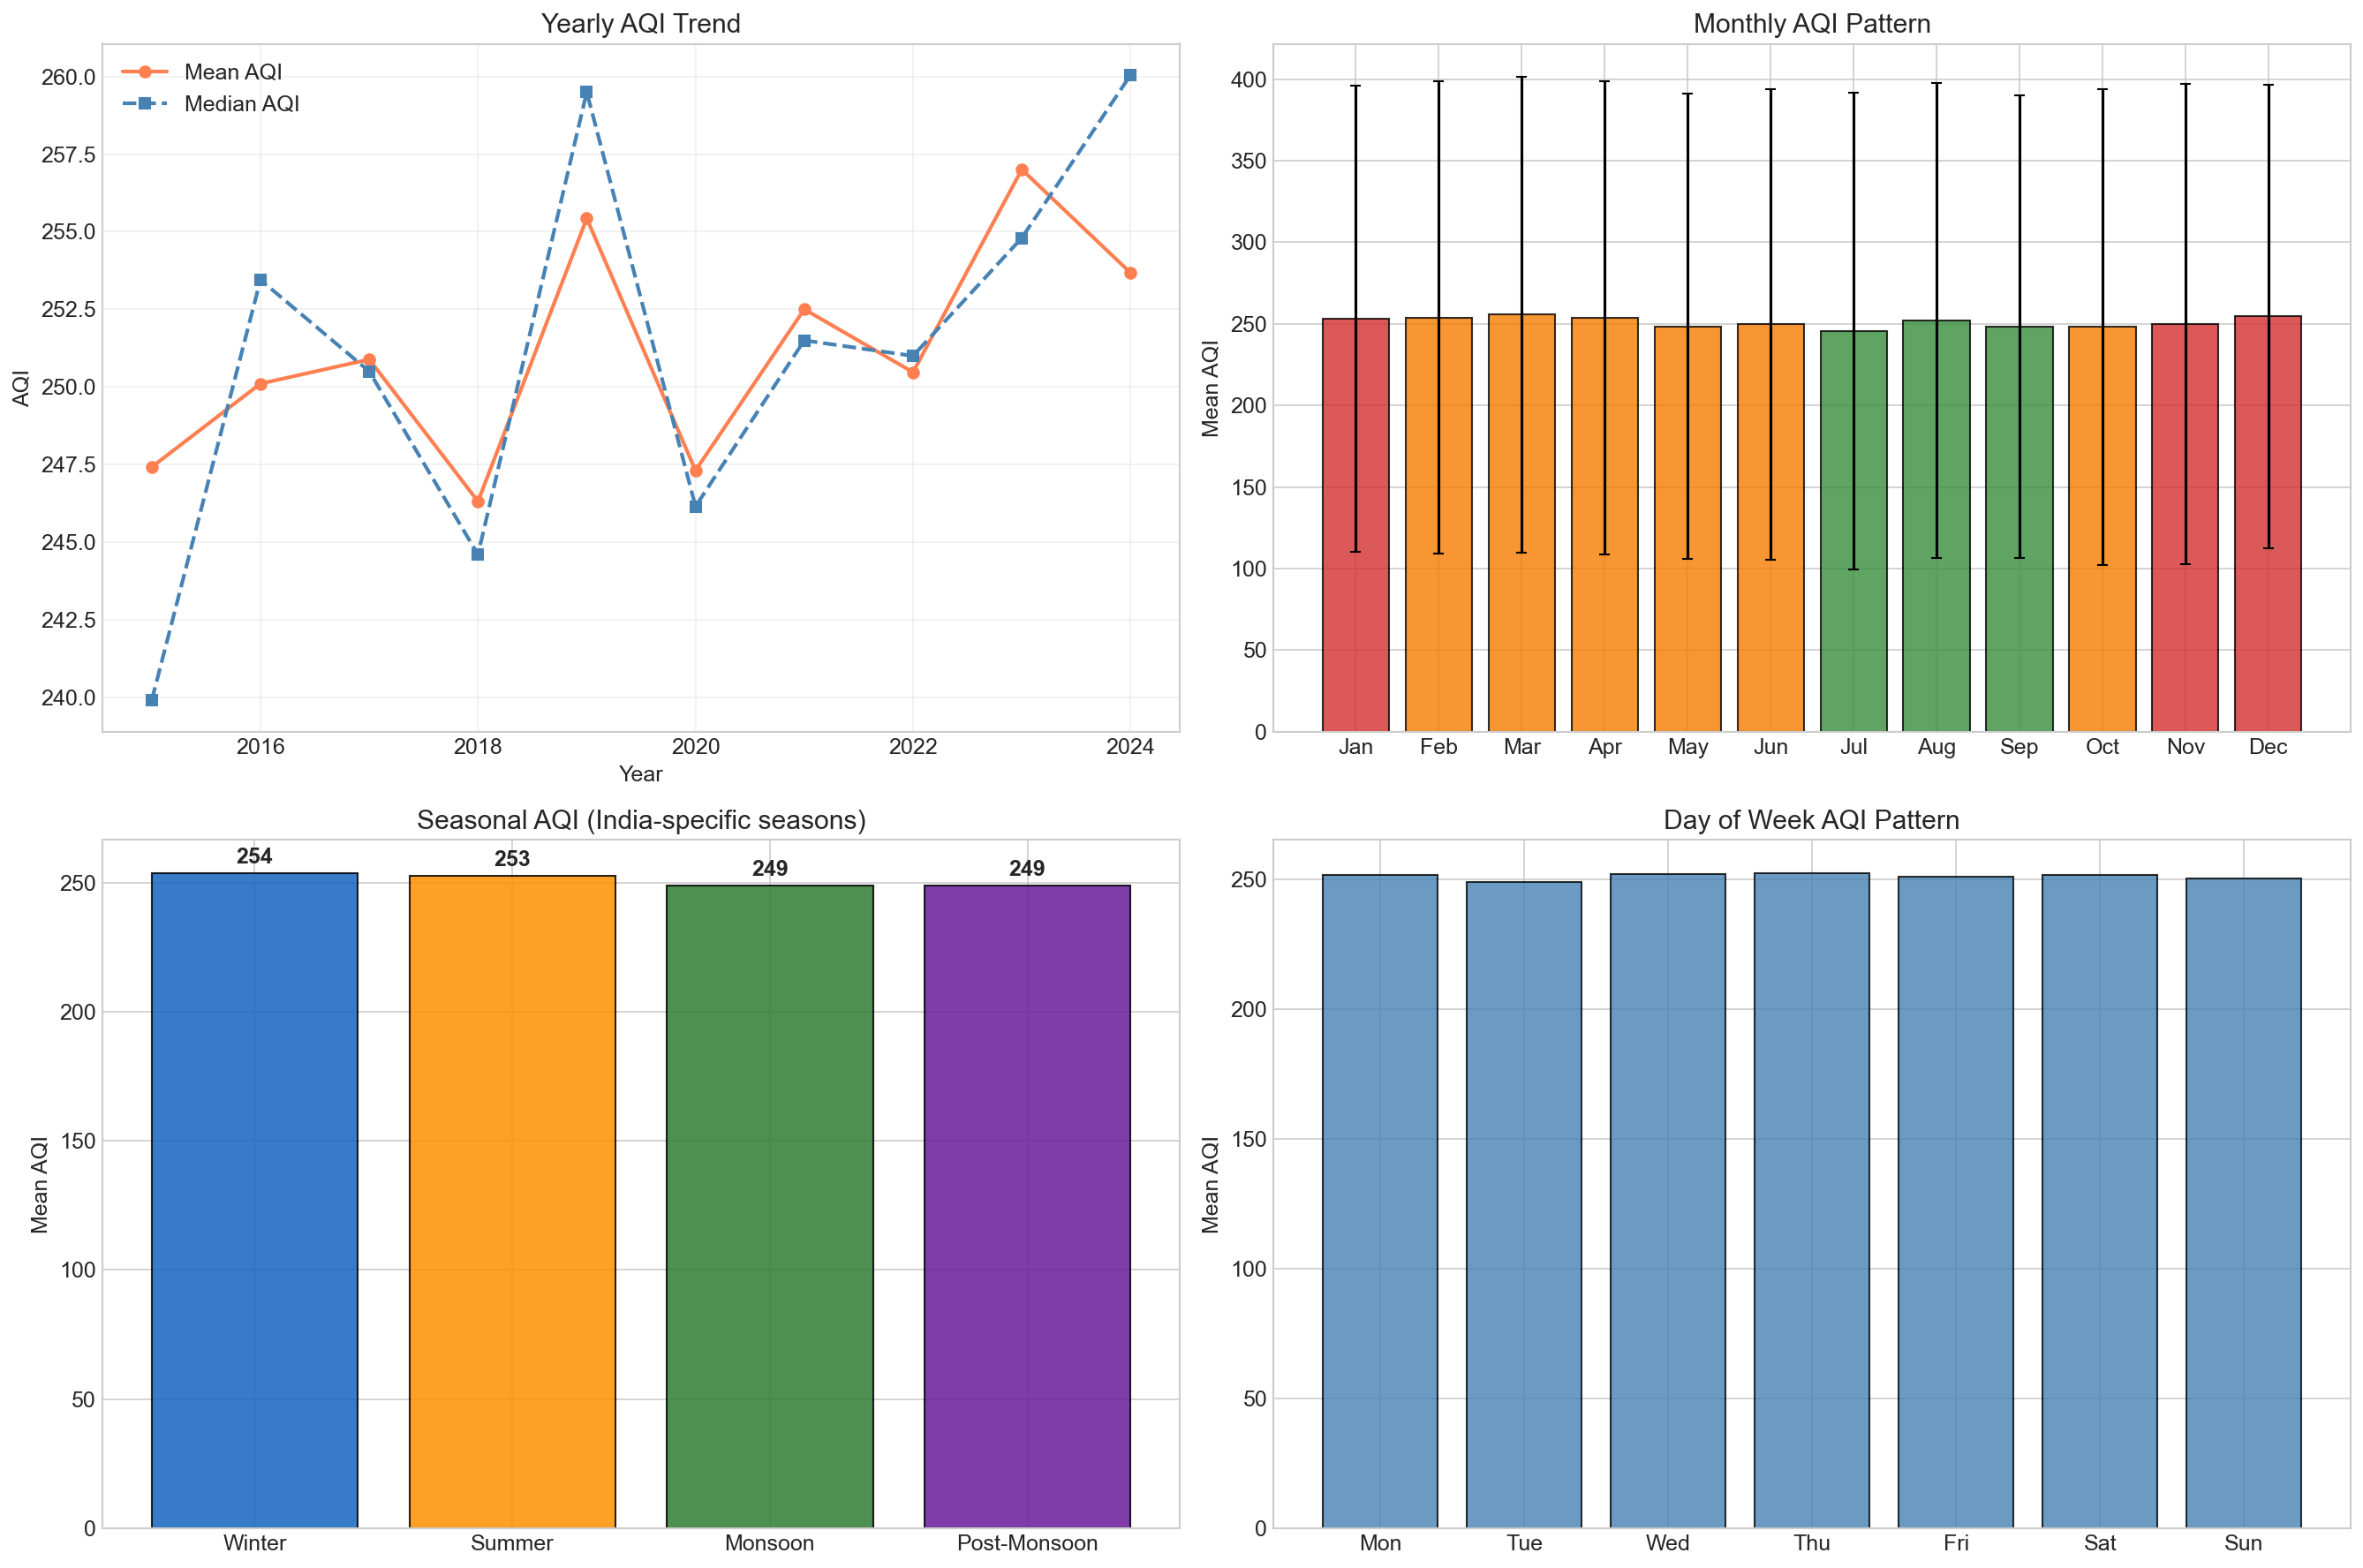
\includegraphics[width=\columnwidth]{figures/06_temporal_trends.png}
\caption{Temporal decomposition of AQI values by year, month, India-specific season, and day of week. Winter months (November--February) exhibit mean AQI values 60--80\% higher than the monsoon trough (July--September). Day-of-week effects are negligible.}
\label{fig:temporal}
\end{figure}

Temporal analysis (Fig.~\ref{fig:temporal}) exposes strong seasonality aligned with India's meteorological calendar. Winter months (December--February) produce the highest AQI readings (mean $\approx$ 200) due to temperature inversions that trap pollutants near the surface, reduced atmospheric mixing height, and increased biomass burning for heating. The monsoon season (June--September) provides substantial relief (mean AQI $\approx$ 90) through particulate washout by precipitation and enhanced ventilation. A sharp post-monsoon spike in October--November corresponds to crop stubble burning in Punjab and Haryana, whose smoke plumes are transported across the Indo-Gangetic Plain \cite{ganguly2020}.

\begin{figure}[!t]
\centering
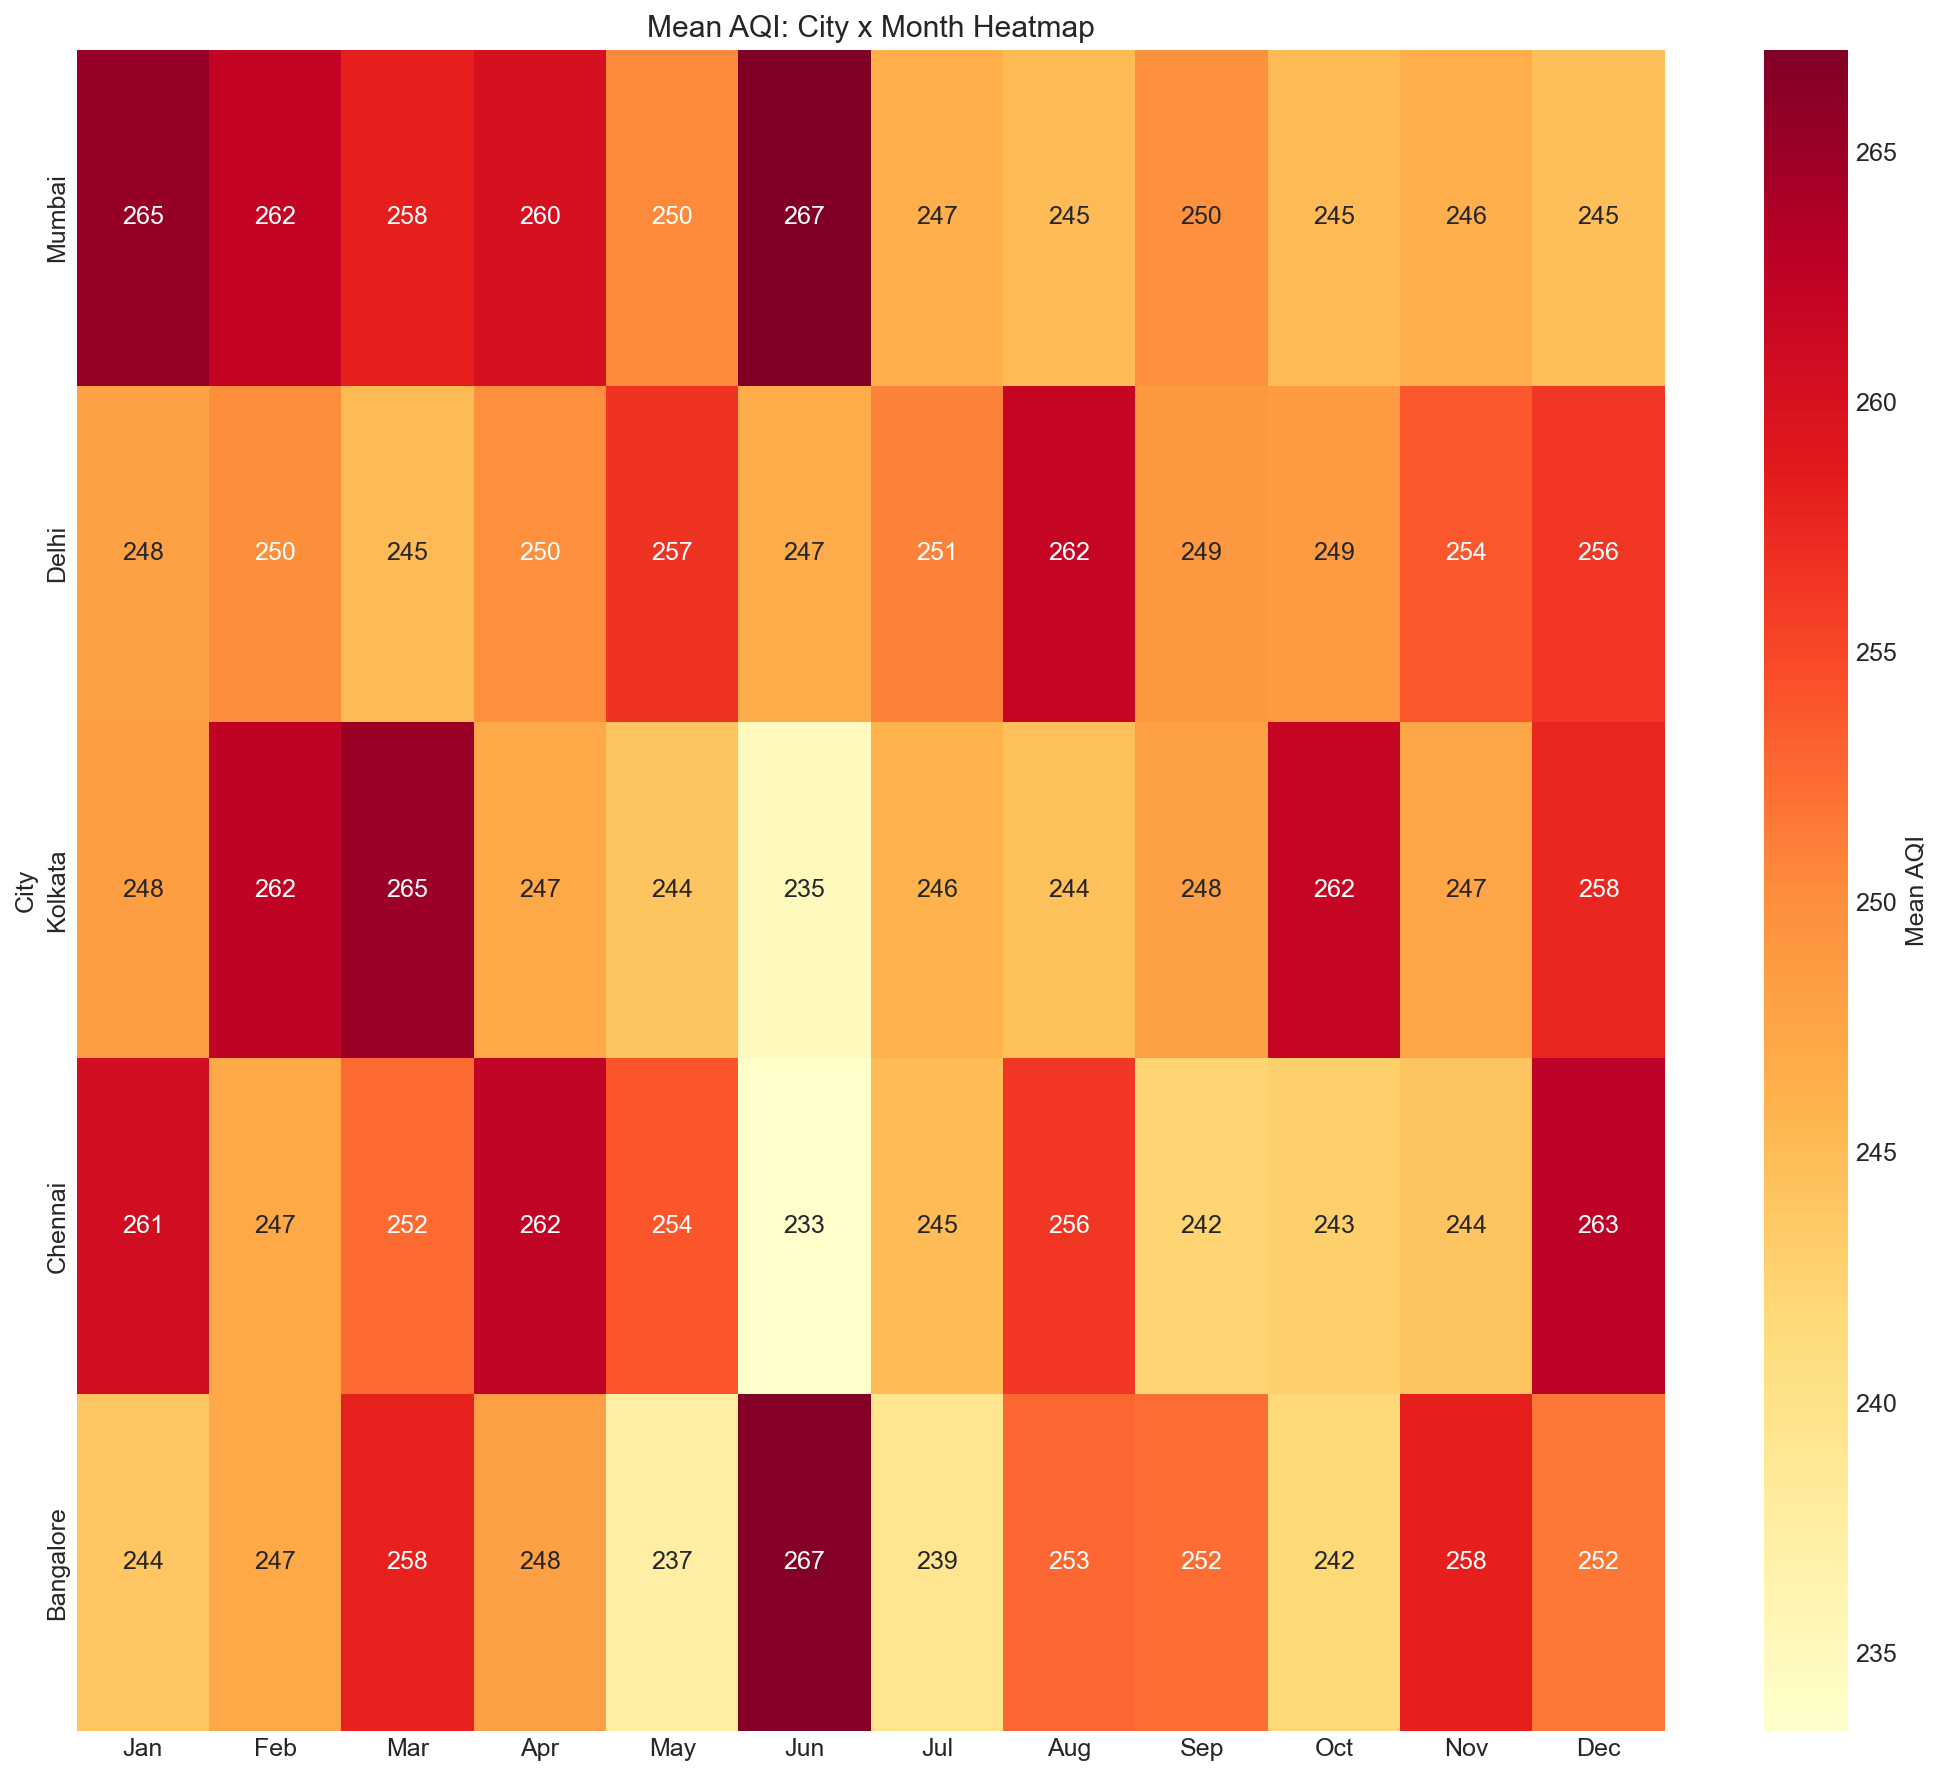
\includegraphics[width=\columnwidth]{figures/09_city_month_heatmap.png}
\caption{City $\times$ month heatmap of mean AQI values. The Indo-Gangetic Plain cities (Delhi, Patna, Lucknow) exhibit the most severe winter pollution, while coastal and southern cities maintain relatively lower and more uniform AQI throughout the year.}
\label{fig:heatmap}
\end{figure}

Geographic patterns (Fig.~\ref{fig:heatmap}) confirm that Delhi, Patna, and Lucknow---all situated in the landlocked Indo-Gangetic basin---suffer the most severe winter pollution episodes, while coastal cities (Thiruvananthapuram, Kochi) and elevated northeast cities (Shillong, Aizawl) maintain consistently lower AQI values.

\begin{figure}[!t]
\centering
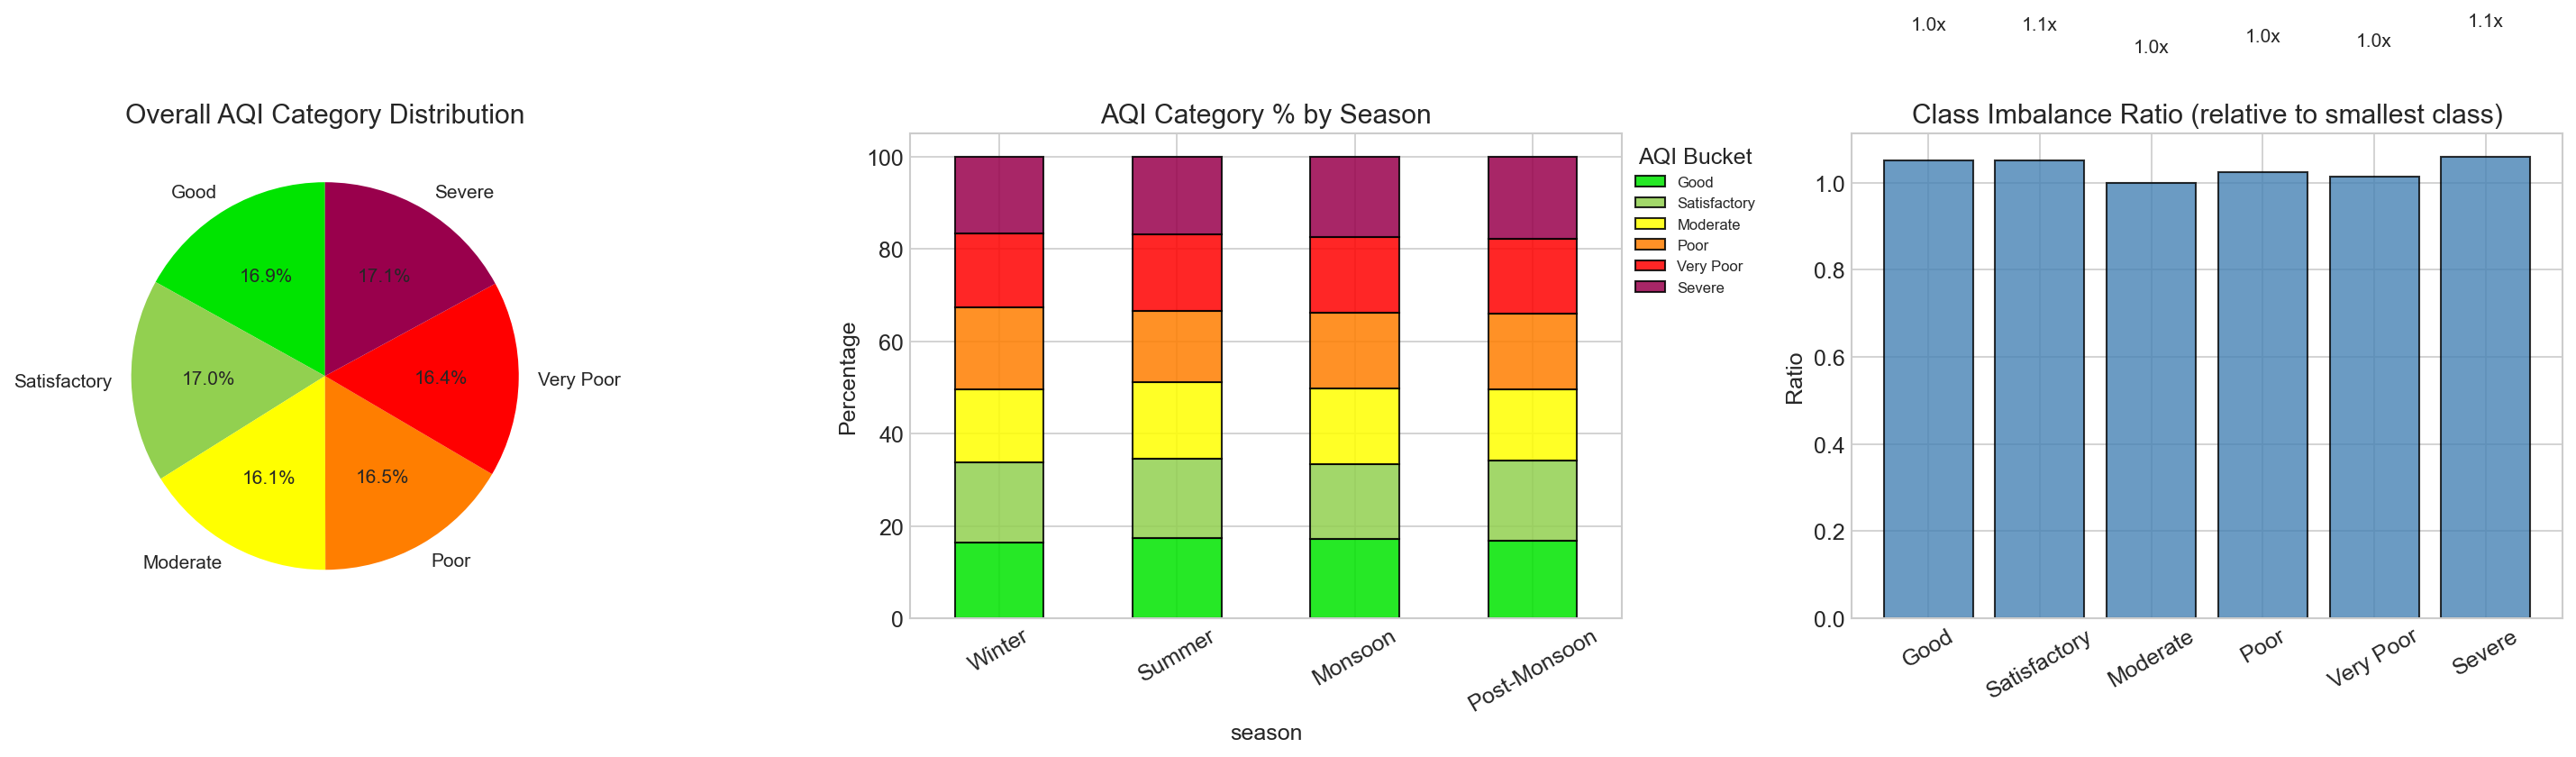
\includegraphics[width=\columnwidth]{figures/10_class_imbalance.png}
\caption{Distribution of AQI categories in the dataset. The Moderate class (37.1\%) dominates, while Good (3.3\%) and Severe (6.7\%) categories are substantially underrepresented, necessitating class balancing for classification tasks.}
\label{fig:imbalance}
\end{figure}

The six AQI categories (Fig.~\ref{fig:imbalance}) are markedly imbalanced: Moderate (37.1\%) and Satisfactory (29.2\%) together account for 66.3\% of observations, while Good (3.3\%) is underrepresented by a factor of 11.3 relative to the majority class.

\subsection{Missing Value Imputation}

A multi-tier imputation strategy was employed to address the 88{,}488 missing cells while preserving temporal autocorrelation and inter-pollutant relationships:

\textit{Stage 1: Linear Interpolation.} Within each city group, linear interpolation was applied to fill gaps of three or fewer consecutive days, leveraging the strong day-to-day autocorrelation in ambient pollutant concentrations.

\textit{Stage 2: KNN Imputation.} Remaining missing values were filled using $k$-nearest neighbours imputation ($k = 5$, distance-weighted), which exploits cross-pollutant correlations---for instance, using PM\textsubscript{10} and CO readings to infer missing PM\textsubscript{2.5} values.

\textit{Stage 3: Sparse Row Removal.} Records with more than 50\% of pollutant columns still missing after the first two stages were removed, as insufficient information remained for reliable imputation. This step removed 1{,}481 rows.

After imputation, 24{,}850 complete records remained (84.2\% retention from the original 29{,}531).

\subsection{Outlier Treatment}

\begin{figure}[!t]
\centering
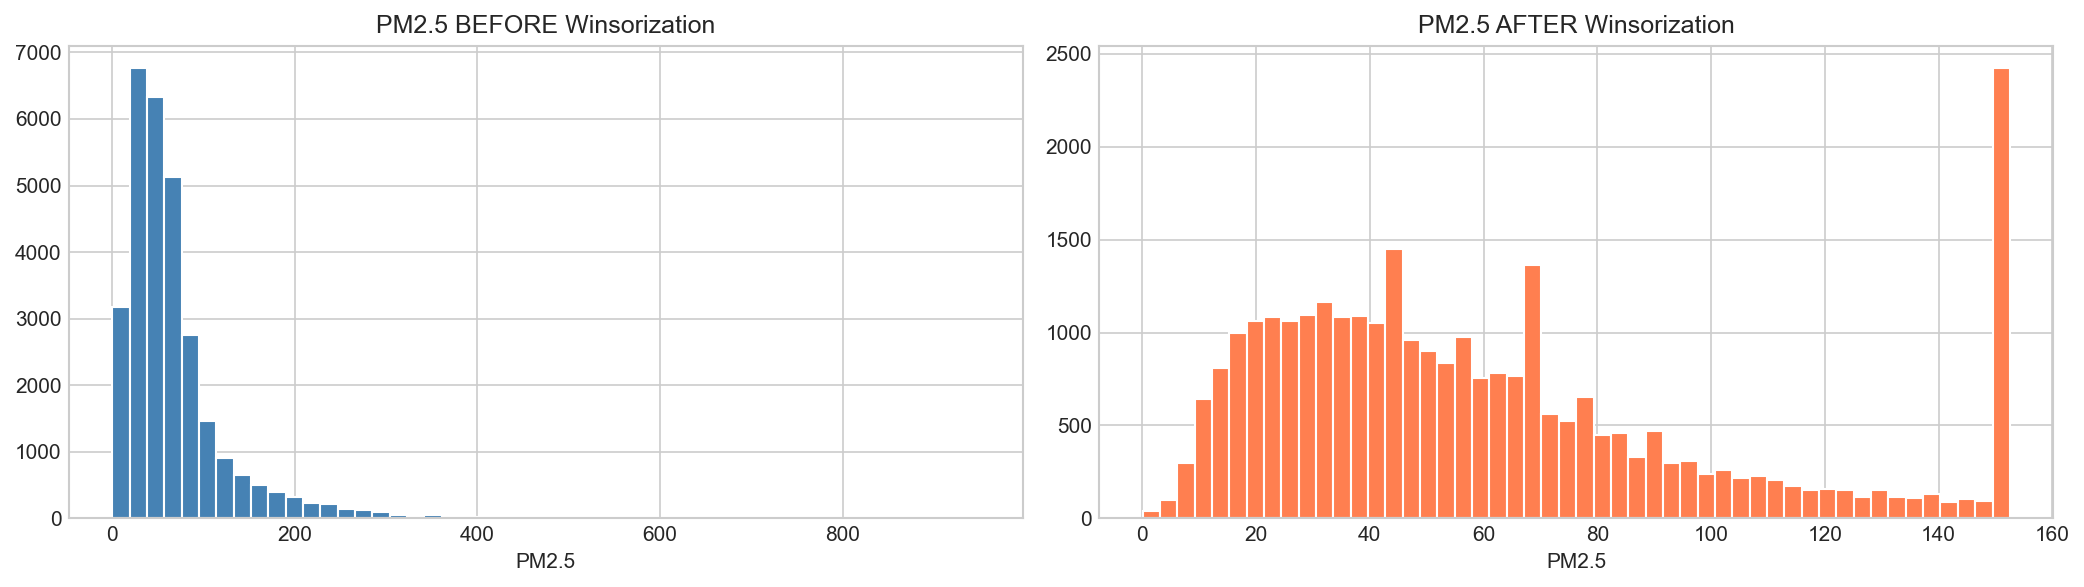
\includegraphics[width=\columnwidth]{figures/12_winsorization_pm25.png}
\caption{Effect of winsorization on PM\textsubscript{2.5} distribution. Values beyond Q1 $-$ 1.5$\times$IQR and Q3 $+$ 1.5$\times$IQR are capped (not removed), preserving genuine high-pollution events while reducing the influence of extreme outliers on model training.}
\label{fig:winsorization}
\end{figure}

Outlier values were addressed through winsorization at the 1.5$\times$IQR threshold (Fig.~\ref{fig:winsorization}). Unlike hard removal, winsorization caps extreme values at the lower and upper fences, preserving the sample size and the representation of genuine high-pollution episodes. This choice is motivated by the domain context: very high PM\textsubscript{2.5} readings ($>$300~$\mu$g/m$^3$) in Delhi during winter are scientifically valid and should not be discarded, but their raw magnitude can disproportionately influence least-squares-based objectives.

\subsection{AQI Validation}

\begin{figure}[!t]
\centering
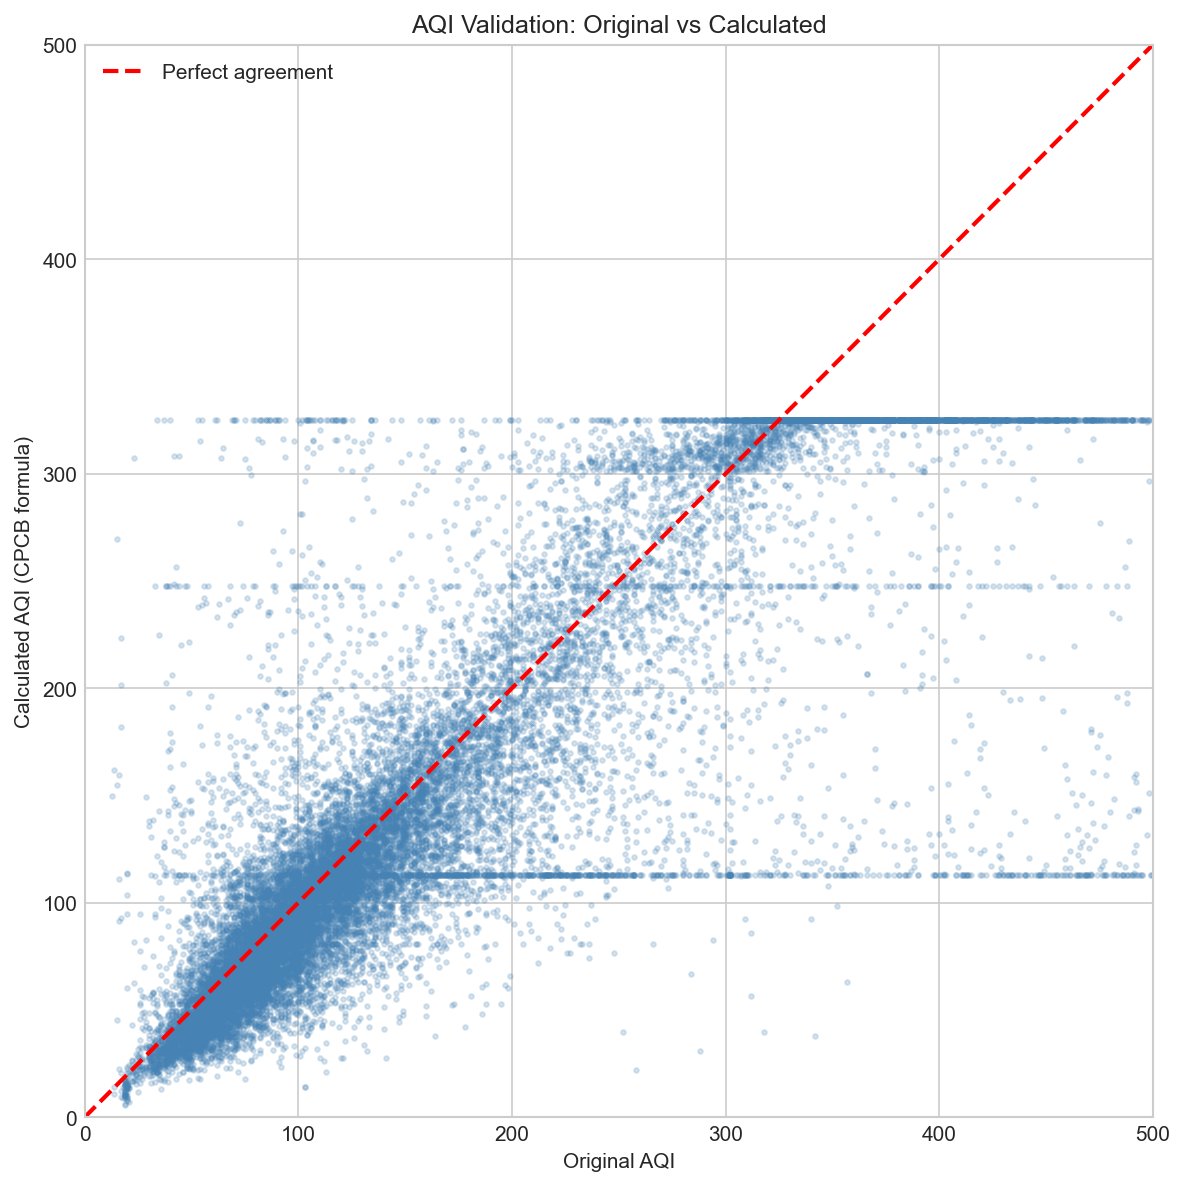
\includegraphics[width=\columnwidth]{figures/13_aqi_validation.png}
\caption{Scatter plot of original dataset AQI values versus AQI recomputed from pollutant concentrations using the CPCB formula. Strong agreement along the diagonal validates dataset integrity, with a median absolute deviation of 17.1 AQI units.}
\label{fig:validation}
\end{figure}

To verify dataset integrity, the AQI was recomputed from pollutant concentrations using the CPCB piecewise linear formula (Fig.~\ref{fig:validation}). The median absolute deviation between the provided and computed AQI was 17.1 units, and 63.7\% of records showed more than 10\% divergence---attributable to the max-of-sub-indices calculation, where the dominant pollutant can shift between time periods and data sources.

% ============================================================
% IV. METHODOLOGY
% ============================================================
\section{Methodology}

\subsection{Feature Engineering}

Twelve raw pollutant measurements were transformed into a 141-dimensional feature vector through four categories of engineered features:

\textit{Temporal Features (7).} Year, month, day of week, day of year, quarter, binary weekend indicator, and India-specific season (Winter: Dec--Feb, Summer: Mar--May, Monsoon: Jun--Sep, Post-Monsoon: Oct--Nov).

\textit{Lag Features (72).} For each of the 12 pollutant columns, lagged values at offsets of 1, 2, 3, 7, 14, and 30 days were computed. Lag features capture the autoregressive nature of atmospheric pollution: PM\textsubscript{2.5} concentrations today are strongly predictive of tomorrow's values due to the multi-day persistence of pollution episodes under stagnant atmospheric conditions.

\textit{Rolling Window Statistics (48).} Rolling mean and standard deviation were computed over windows of 3, 7, 14, and 30 days for six key pollutants (PM\textsubscript{2.5}, PM\textsubscript{10}, NO\textsubscript{2}, SO\textsubscript{2}, CO, O\textsubscript{3}). A one-day shift was applied prior to rolling computation to prevent target leakage. These features encode both the recent pollution trend (rolling mean) and its volatility (rolling standard deviation).

\textit{Pollutant Ratios (2).} The PM\textsubscript{2.5}/PM\textsubscript{10} ratio distinguishes combustion-dominated pollution (high ratio, fine particles from vehicles and biomass) from dust-dominated events (low ratio, coarse particles from construction and wind erosion). The NO\textsubscript{2}/NO ratio serves as an indicator of photochemical oxidation state and traffic proximity.

After lag feature computation, rows with insufficient history (first 30 days per city) were dropped, and one label-encoded city feature was appended, yielding the final 141-feature matrix.

\subsection{Data Splitting Strategy}

\begin{figure}[!t]
\centering
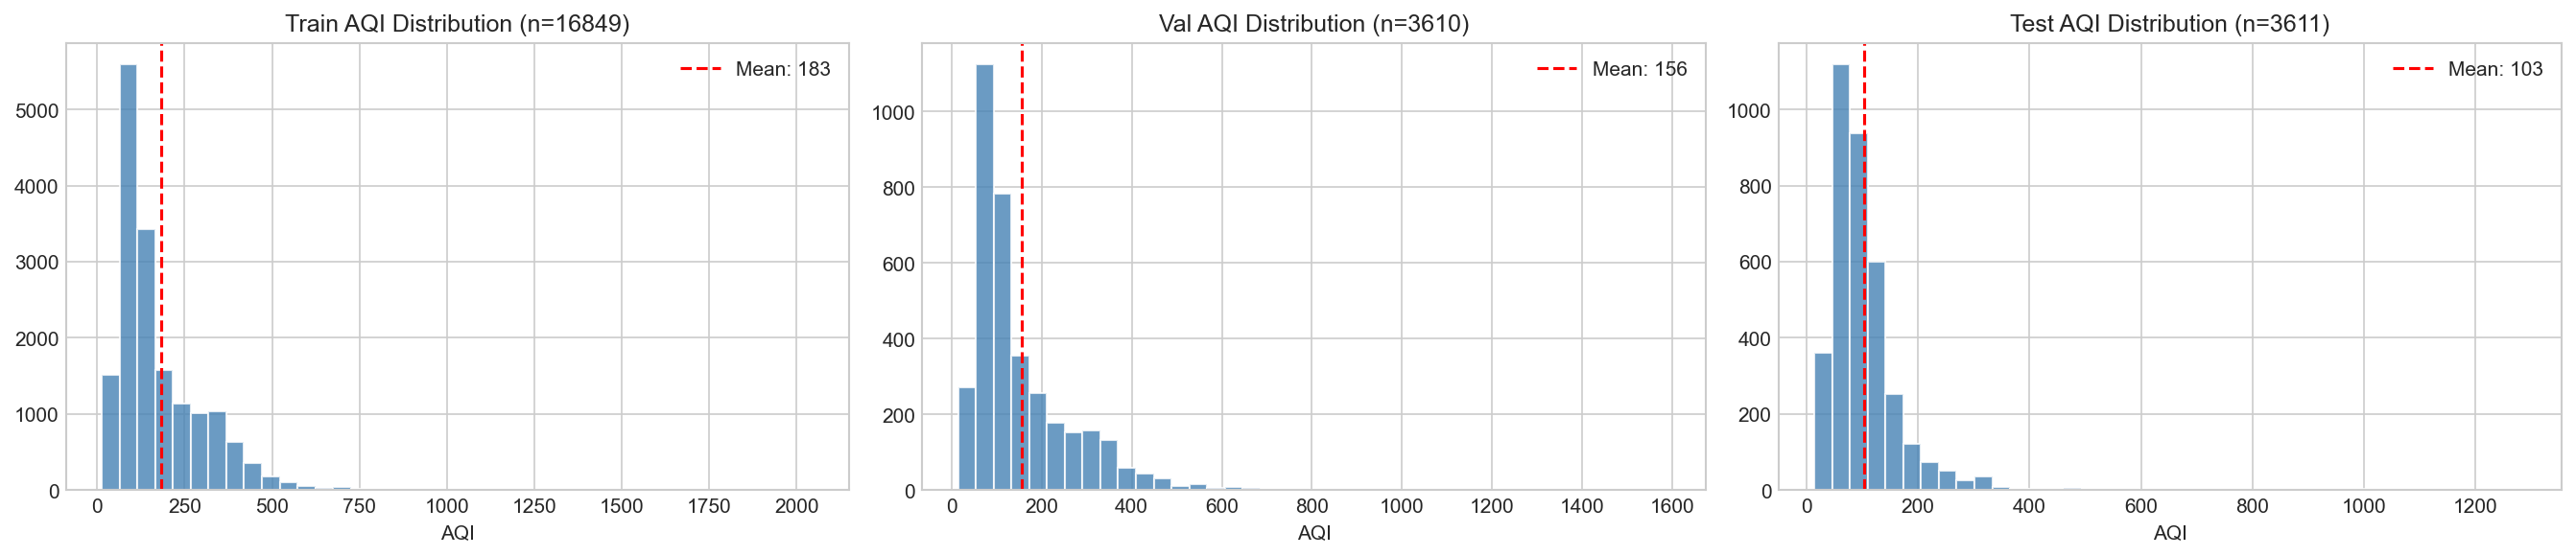
\includegraphics[width=\columnwidth]{figures/14_split_distributions.png}
\caption{AQI distributions across temporal data splits. The training set (70\%, 2015--Aug 2019), validation set (15\%, Aug 2019--Feb 2020), and test set (15\%, Feb--Jul 2020) maintain comparable distributional characteristics, with the test set additionally capturing the COVID-19 lockdown AQI reduction.}
\label{fig:splits}
\end{figure}

A strictly temporal split was applied (Fig.~\ref{fig:splits}): training data comprised the earliest 70\% of records per city (16{,}849 samples, January 2015 -- August 2019), the validation set the next 15\% (3{,}610 samples, August 2019 -- February 2020), and the test set the final 15\% (3{,}611 samples, February -- July 2020). Random shuffling was explicitly avoided, as it would introduce future-to-past information leakage through the lag and rolling features. Per-city temporal integrity was verified to ensure no city's test observations preceded its training observations.

The test period (February--July 2020) encompasses India's national COVID-19 lockdown (March 25 -- May 31, 2020), during which vehicular traffic dropped by 70--90\% and industrial emissions decreased by 40--60\% \cite{mahato2020, sharmaetal2020}. This provides a natural experiment for evaluating whether the models have learned genuine pollutant--AQI relationships or have merely memorised temporal patterns.

\subsection{Regression Models}

Eight regression models were trained to predict continuous AQI values, spanning three levels of complexity:

\textit{Linear Baselines.} Ridge regression (L2 penalty) and Lasso regression (L1 penalty with implicit feature selection) serve as baselines for quantifying the non-linear component of the prediction task.

\textit{Tree-Based Models.} Decision Tree (single tree, no ensemble), Random Forest \cite{breiman2001} (bagging of 100 decorrelated trees), and three gradient boosting variants: XGBoost \cite{chen2016} (second-order gradient optimisation), LightGBM \cite{ke2017} (histogram-based splitting, leaf-wise growth), and CatBoost \cite{prokhorenkova2018} (ordered boosting with symmetric trees).

\textit{Kernel Method.} Support Vector Regression (SVR) with a radial basis function (RBF) kernel \cite{cortes1995}, which projects the feature space into a higher-dimensional manifold to capture non-linear relationships.

All features were standardised using a StandardScaler fitted on the training set for distance-sensitive models (SVR, Ridge, Lasso). Tree-based models received unscaled features. Default hyperparameters from the respective libraries (scikit-learn 1.3, XGBoost 2.0, LightGBM 4.0, CatBoost 1.2) were used for the initial comparison; the top-performing models were subsequently tuned via Bayesian optimisation (Section~IV-F).

\subsection{Classification Models}

Seven classification models were trained to predict the six-class AQI category. The training set exhibits a 11.3:1 imbalance ratio between the largest (Moderate, 6{,}245 samples) and smallest (Good, 553 samples) classes. Two class-balancing strategies were compared:

\textit{SMOTE.} The Synthetic Minority Over-sampling Technique \cite{chawla2002} was applied to the training set only, expanding it from 16{,}849 to 37{,}470 samples (6{,}245 per class). SMOTE generates synthetic instances along line segments connecting minority-class neighbours in feature space.

\textit{Class Weights.} As an alternative, CatBoost's built-in \texttt{class\_weights} parameter was used to penalise minority-class misclassifications inversely proportional to class frequency, without generating synthetic data.

The classifier suite comprised Logistic Regression, Decision Tree, Random Forest, XGBoost, LightGBM, CatBoost with SMOTE, and CatBoost with class weights.

\subsection{Deep Learning Architectures}

Five recurrent and hybrid architectures were designed to process raw pollutant sequences without pre-engineered lag or rolling features:

\textit{Input Representation.} A sliding window of 14 consecutive days was applied to the 7 core AQI pollutants (PM\textsubscript{2.5}, PM\textsubscript{10}, NO\textsubscript{2}, SO\textsubscript{2}, CO, O\textsubscript{3}, NH\textsubscript{3}), producing 3D input tensors of shape (samples, 14, 7). Windows were constructed per city to prevent cross-city sequence contamination.

\textit{Architectures:}
\begin{itemize}
    \item \textbf{Vanilla LSTM}: LSTM(64 units) $\rightarrow$ Dropout(0.2) $\rightarrow$ Dense(32, ReLU) $\rightarrow$ Dense(1).
    \item \textbf{Stacked LSTM}: LSTM(64) $\rightarrow$ LSTM(32) $\rightarrow$ Dropout(0.2) $\rightarrow$ Dense(32) $\rightarrow$ Dense(1).
    \item \textbf{Bidirectional LSTM}: BiLSTM(64) $\rightarrow$ Dropout(0.2) $\rightarrow$ Dense(32) $\rightarrow$ Dense(1).
    \item \textbf{Conv1D-LSTM}: Conv1D(64, kernel=3) $\rightarrow$ MaxPool(2) $\rightarrow$ LSTM(64) $\rightarrow$ Dense(32) $\rightarrow$ Dense(1).
    \item \textbf{GRU}: GRU(64) $\rightarrow$ Dropout(0.2) $\rightarrow$ Dense(32) $\rightarrow$ Dense(1).
\end{itemize}

All architectures used the Adam optimiser (learning rate $= 10^{-3}$), MSE loss, a maximum of 100 epochs with early stopping (patience = 15 epochs), and a ReduceLROnPlateau callback (factor = 0.5, patience = 5). Input features were standardised using a StandardScaler fitted exclusively on the training sequences.

\subsection{Hyperparameter Optimisation}

The top three regression models (LightGBM, CatBoost, XGBoost) were optimised using Optuna \cite{akiba2019} with the Tree-structured Parzen Estimator (TPE) sampler. Each model underwent 50 trials, with the objective of maximising $R^2$ on the validation set. Search spaces included learning rate ($[0.01, 0.3]$, log scale), number of estimators ($[100, 1000]$), tree depth or leaf count, regularisation terms ($\lambda_1$, $\lambda_2 \in [10^{-8}, 10]$, log scale), and subsampling ratios ($[0.5, 1.0]$). Final models were retrained on the combined training and validation sets and evaluated on the held-out test set.

\subsection{SHAP Explainability Framework}

Post-hoc explanations were generated using the TreeExplainer algorithm \cite{lundberg2020}, which computes exact Shapley values in polynomial time for tree-ensemble models. A stratified sample of 500 test observations was used for computational tractability. Four complementary analyses were conducted:

\begin{itemize}
    \item \textbf{Bar plot}: Global feature importance ranked by mean $|\text{SHAP}|$ across the sample.
    \item \textbf{Beeswarm plot}: Per-instance SHAP values coloured by feature magnitude, revealing directional relationships.
    \item \textbf{Dependence plots}: SHAP value versus feature value for the top-5 features, with interaction colouring to expose non-linear effects and feature interactions.
    \item \textbf{Per-class SHAP}: Classification model explanations stratified by predicted AQI category, identifying which features differentiate severe from benign air quality predictions.
\end{itemize}

% ============================================================
% V. EXPERIMENTAL RESULTS
% ============================================================
\section{Experimental Results}

\subsection{Regression Results}

\begin{table}[!t]
\centering
\caption{Regression Model Performance on Test Set (3{,}611 Samples)}
\label{tab:regression}
\begin{tabular}{lcccc}
\toprule
\textbf{Model} & \textbf{$R^2$} & \textbf{RMSE} & \textbf{MAE} & \textbf{Time (s)} \\
\midrule
\textbf{LightGBM}  & \textbf{0.9014} & \textbf{23.80} & \textbf{13.22} & 7.29 \\
CatBoost            & 0.8321 & 31.05 & 16.57 & 12.82 \\
SVR (RBF)           & 0.7986 & 34.01 & 18.26 & 79.64 \\
XGBoost             & 0.7492 & 37.95 & 17.19 & 3.24 \\
Random Forest       & 0.7332 & 39.15 & 17.09 & 42.51 \\
Lasso               & 0.5598 & 50.28 & 33.65 & 5.08 \\
Ridge               & 0.5534 & 50.65 & 34.05 & 0.01 \\
Decision Tree       & 0.5154 & 52.76 & 22.94 & 1.58 \\
\bottomrule
\end{tabular}
\end{table}

Table~\ref{tab:regression} presents the test set performance of all eight regression models. LightGBM achieved the highest $R^2$ of 0.9014 with an RMSE of 23.80 AQI units and MAE of 13.22---equivalent to a mean prediction error of approximately 2.6\% of the AQI scale. CatBoost placed second ($R^2 = 0.8321$), followed by SVR ($R^2 = 0.7986$). The gradient boosting family (LightGBM, CatBoost, XGBoost) occupied the top three positions, confirming their suitability for structured environmental tabular data. The linear baselines (Ridge: $R^2 = 0.5534$, Lasso: $R^2 = 0.5598$) explained only 55\% of AQI variance, quantifying the contribution of non-linear feature interactions to approximately 35 percentage points of $R^2$ improvement.

\begin{figure}[!t]
\centering
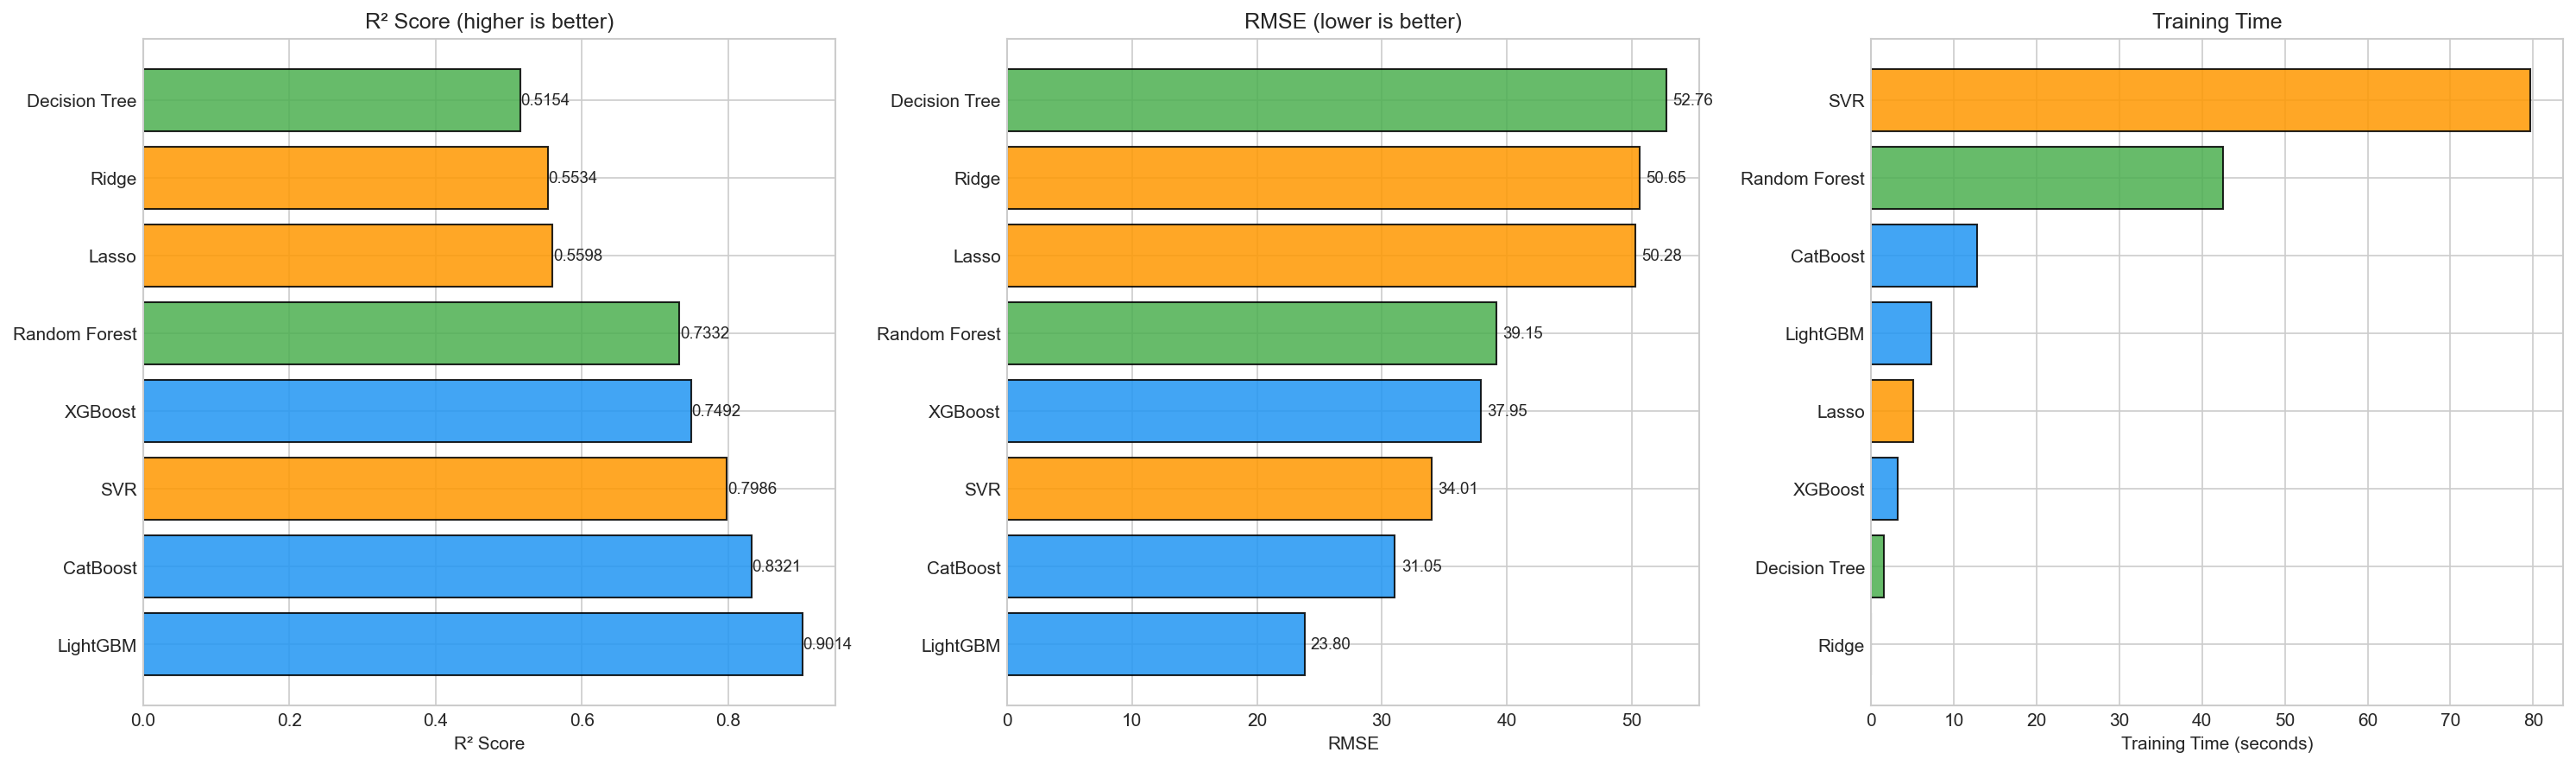
\includegraphics[width=\columnwidth]{figures/15_regression_comparison.png}
\caption{Comparative bar chart of regression model performance across $R^2$, RMSE, and training time. The three gradient boosting variants dominate in predictive accuracy while maintaining sub-15-second training times.}
\label{fig:regbar}
\end{figure}

\begin{figure}[!t]
\centering
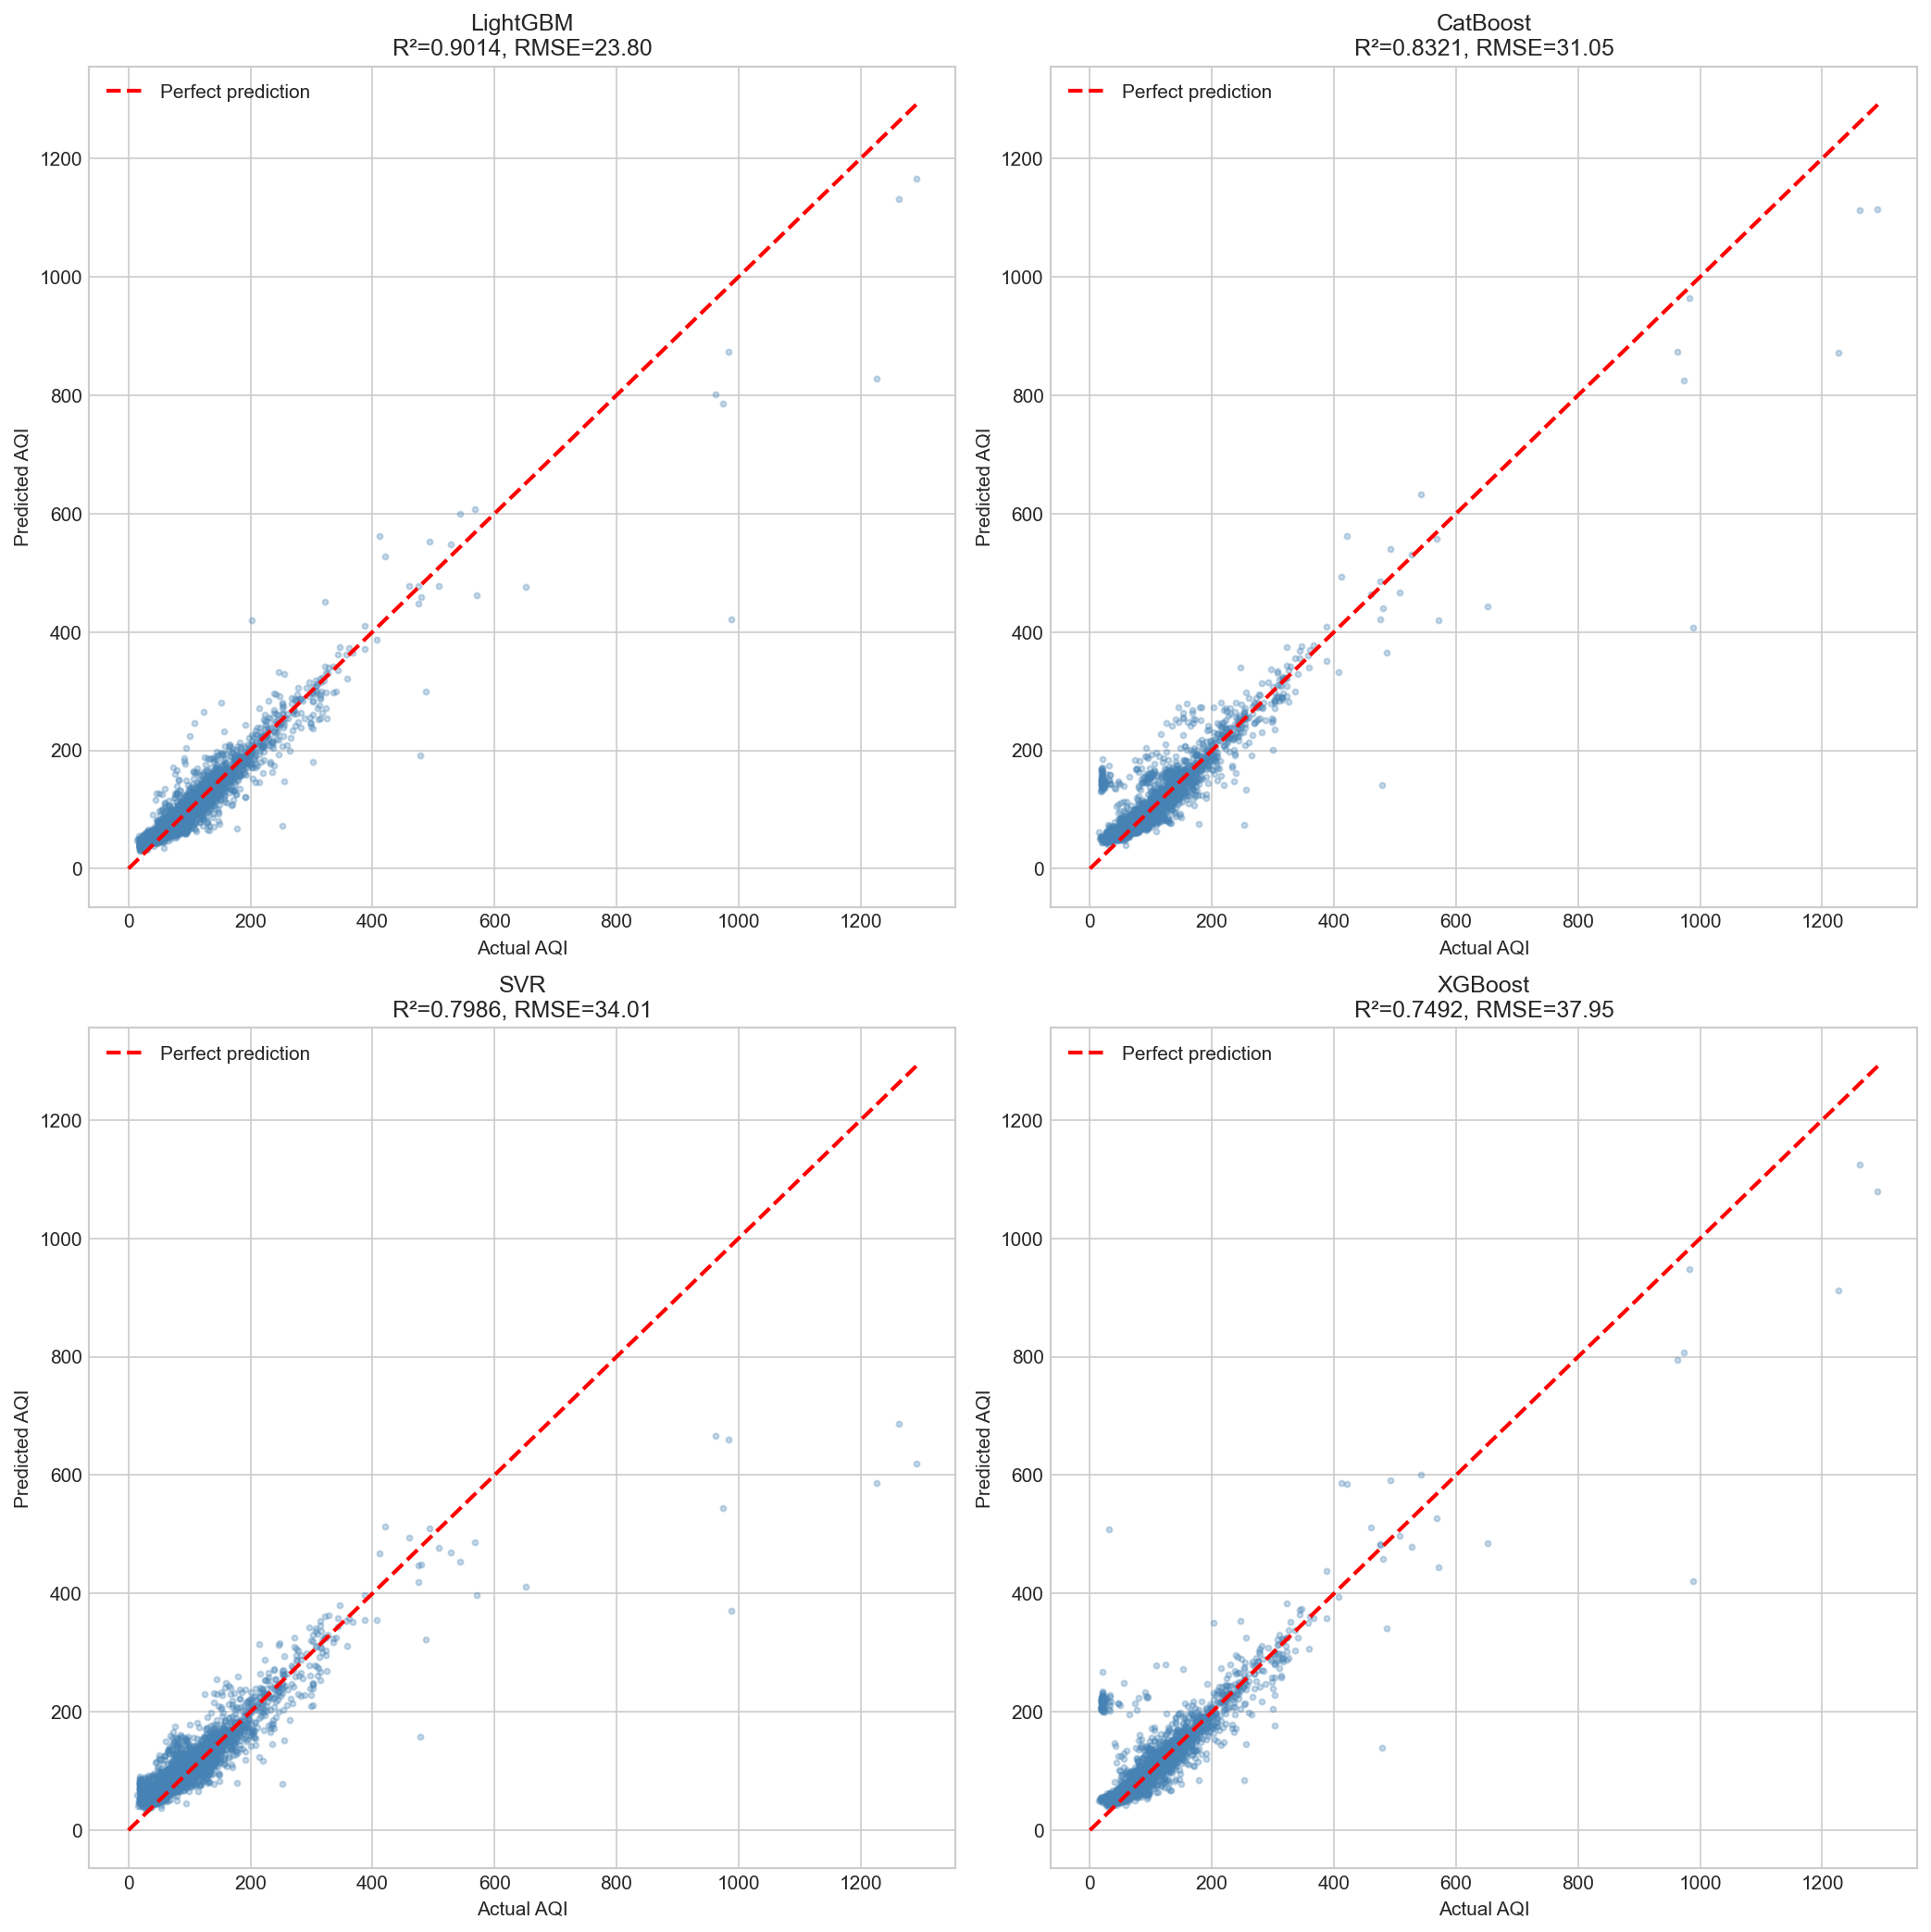
\includegraphics[width=\columnwidth]{figures/16_predicted_vs_actual.png}
\caption{Predicted versus actual AQI scatter plots for the top four regression models. LightGBM exhibits the tightest clustering around the diagonal, with minimal systematic bias across the full AQI range.}
\label{fig:predactual}
\end{figure}

\begin{figure}[!t]
\centering
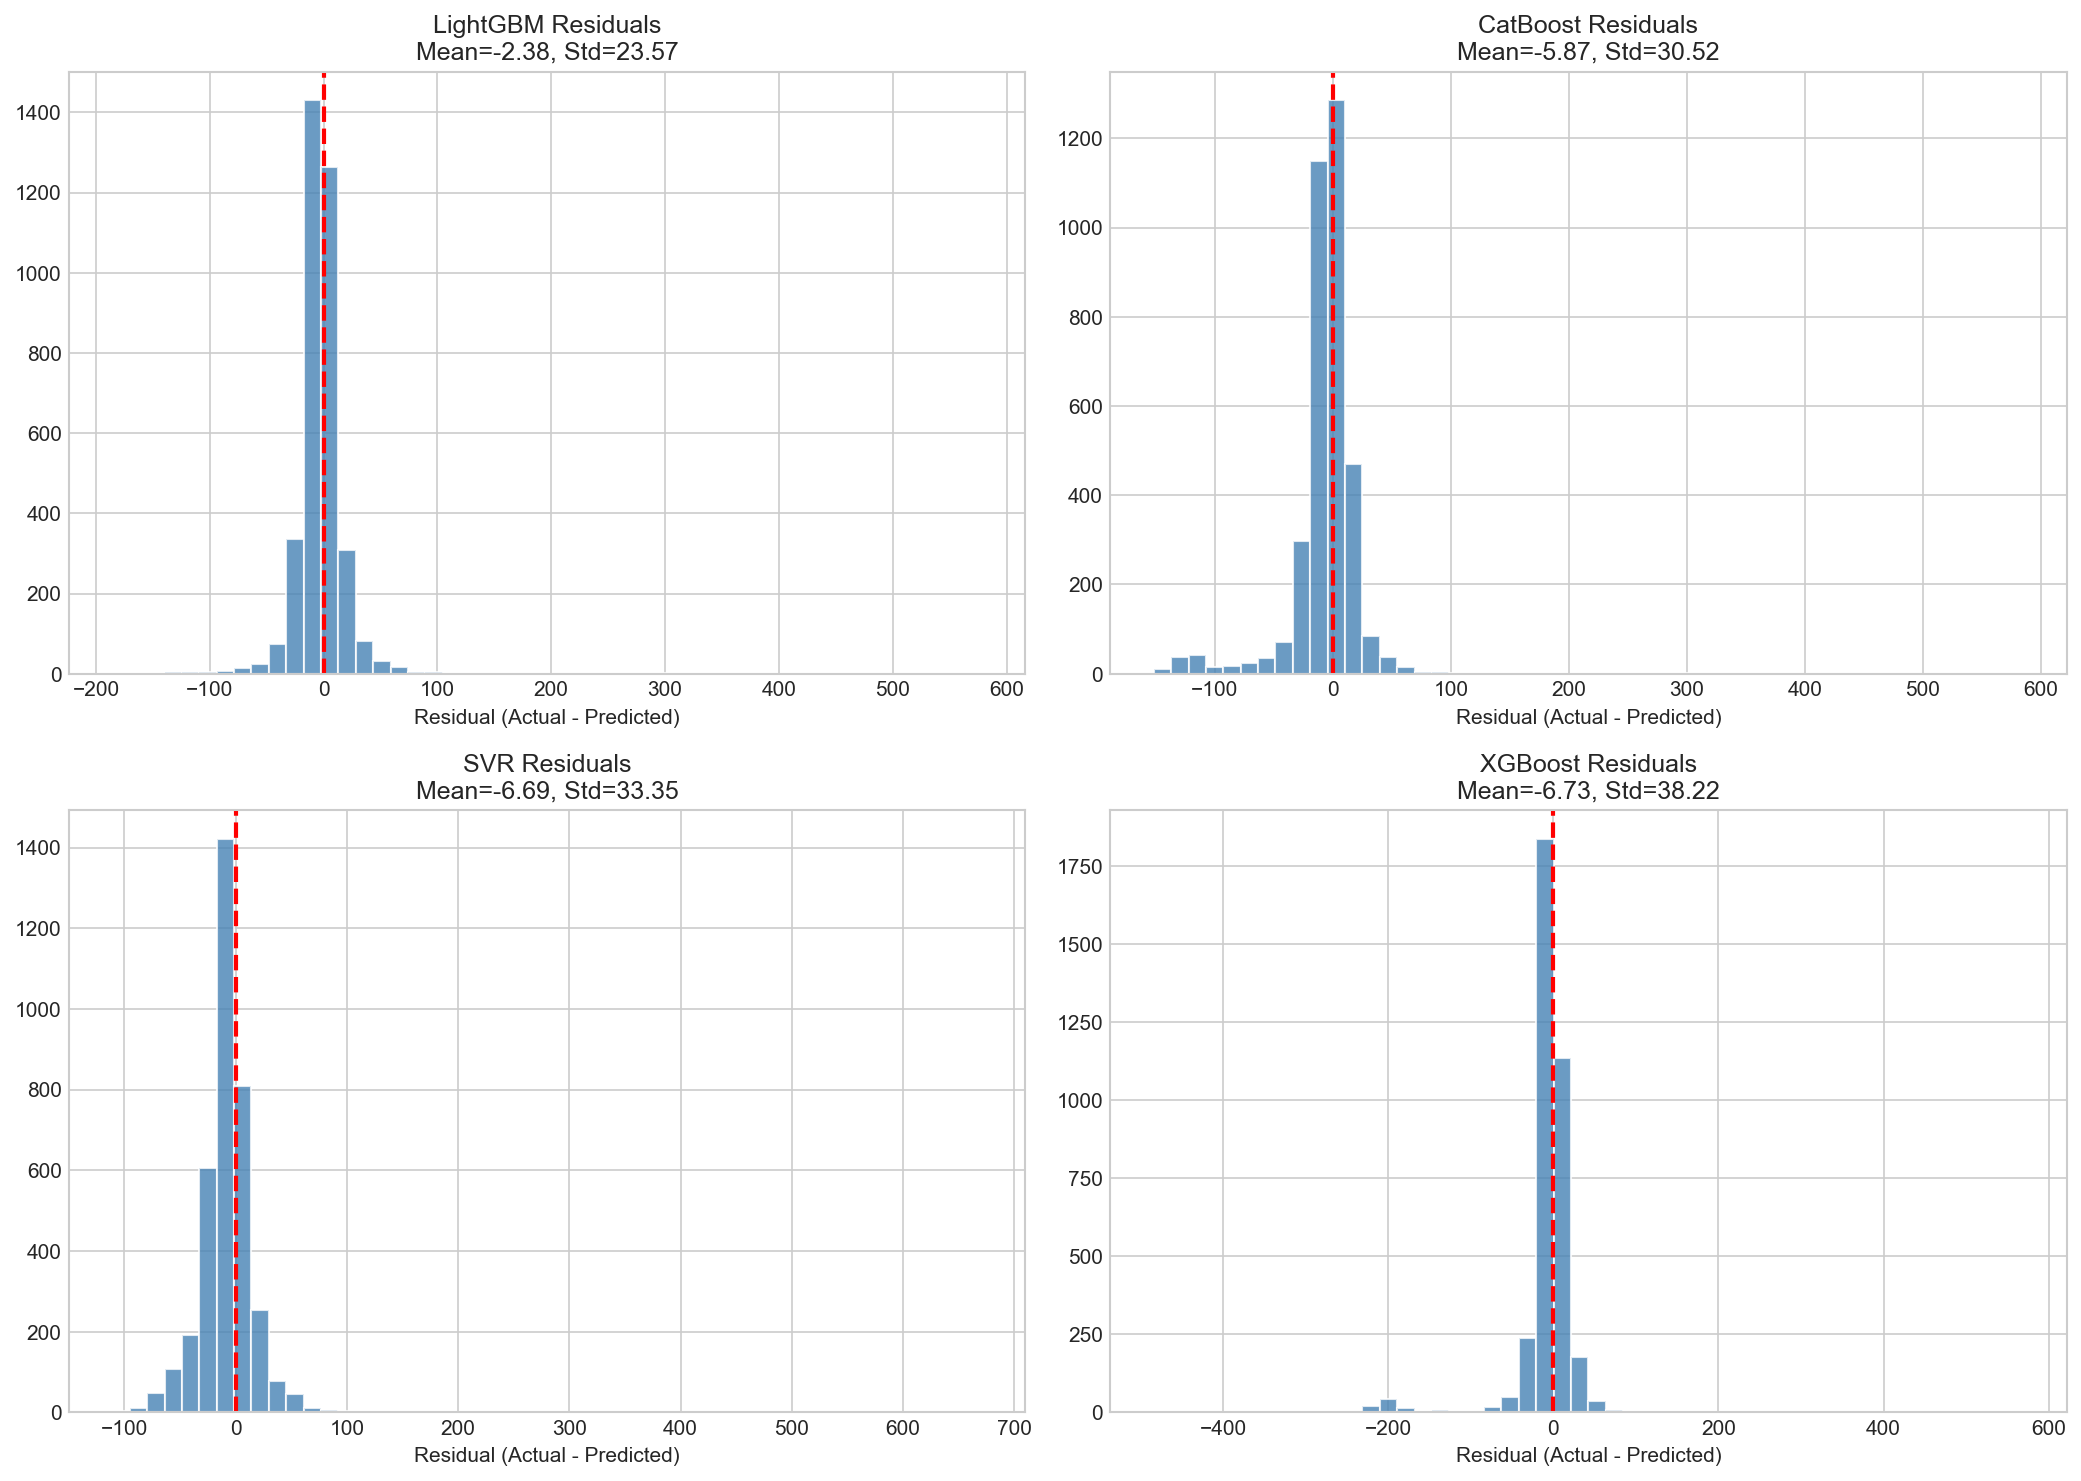
\includegraphics[width=\columnwidth]{figures/17_residuals.png}
\caption{Residual distributions for the top four regression models. All distributions are approximately centred at zero with near-Gaussian profiles, indicating no systematic prediction bias.}
\label{fig:residuals}
\end{figure}

The predicted-versus-actual scatter plots (Fig.~\ref{fig:predactual}) show that LightGBM produces the tightest diagonal clustering across the full 0--500 AQI range, while the Decision Tree exhibits substantial dispersion, particularly at extreme AQI values. Residual analysis (Fig.~\ref{fig:residuals}) confirms that all top-4 models produce approximately zero-mean, symmetric residual distributions with no evidence of heteroscedasticity.

\begin{figure}[!t]
\centering
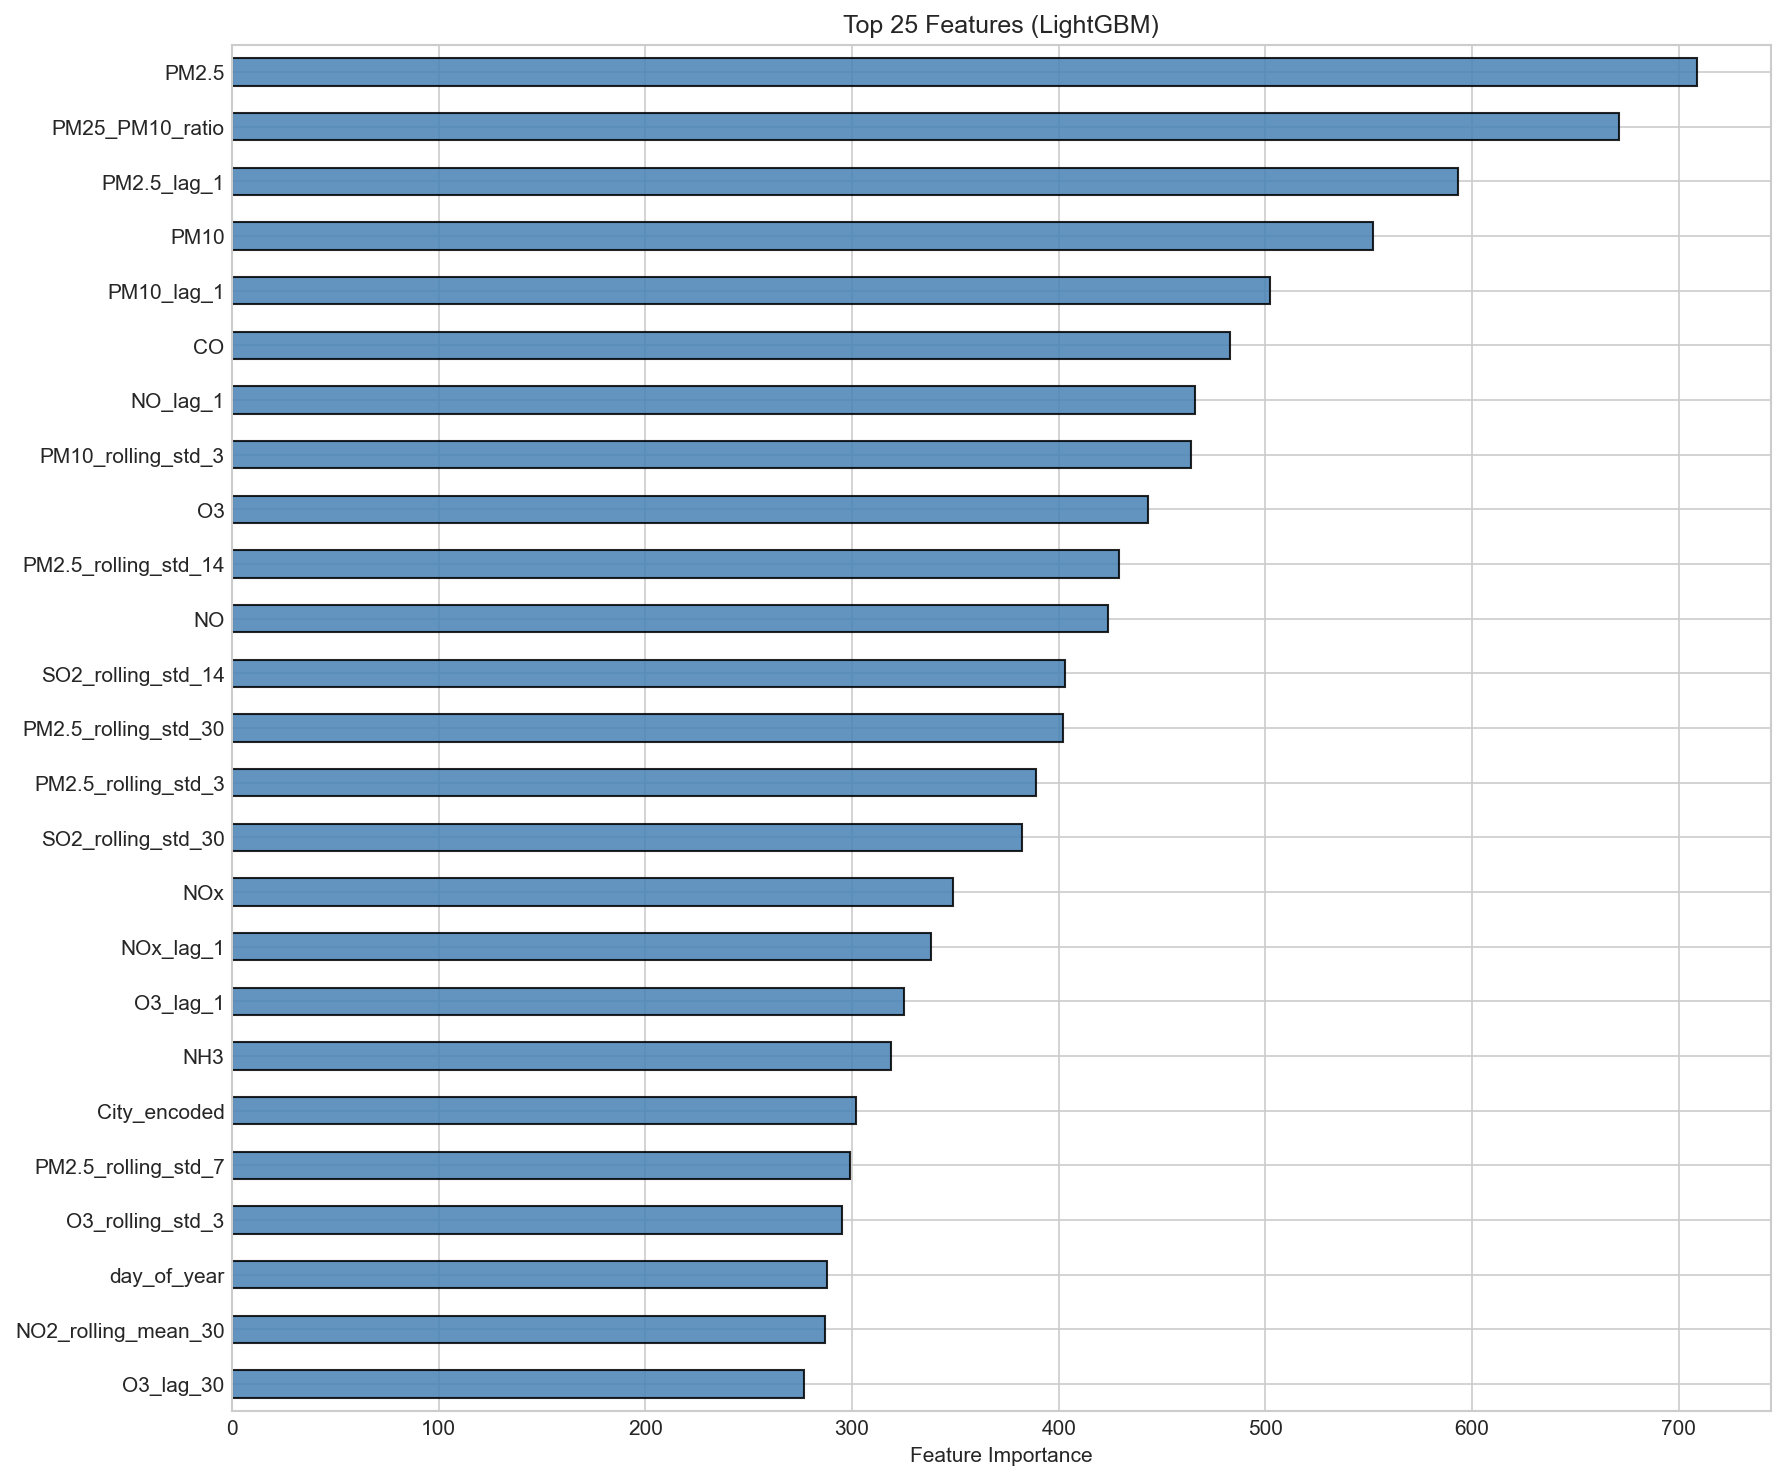
\includegraphics[width=\columnwidth]{figures/18_feature_importance.png}
\caption{Top 25 features by LightGBM split-based importance. Lag and rolling features of PM\textsubscript{2.5} and PM\textsubscript{10} dominate, confirming the central role of particulate matter and temporal persistence in AQI prediction.}
\label{fig:importance}
\end{figure}

LightGBM's native feature importance (Fig.~\ref{fig:importance}) reveals that PM\textsubscript{2.5} and PM\textsubscript{10} lag and rolling features occupy the top positions, with day-of-year and month providing seasonal context. This ordering is consistent with the CPCB AQI formula, where PM\textsubscript{2.5} is the dominant sub-index pollutant in approximately 60--70\% of observations across Indian cities.

\subsection{Classification Results}

\begin{table}[!t]
\centering
\caption{Classification Model Performance on Test Set}
\label{tab:classification}
\begin{tabular}{lccccc}
\toprule
\textbf{Model} & \textbf{Acc.} & \textbf{Bal. Acc.} & \textbf{$F_1^{\text{macro}}$} & \textbf{$\kappa$} & \textbf{Time} \\
\midrule
\textbf{XGBoost}  & \textbf{0.842} & 0.805 & \textbf{0.811} & \textbf{0.755} & 15.1s \\
CatBoost           & 0.831 & \textbf{0.816} & 0.821 & 0.739 & 39.8s \\
LightGBM           & 0.825 & 0.785 & 0.808 & 0.725 & 42.4s \\
CatBoost (wt.)     & 0.804 & 0.803 & 0.791 & 0.704 & 26.2s \\
Random Forest      & 0.772 & 0.741 & 0.744 & 0.641 & 5.9s \\
Decision Tree      & 0.715 & 0.717 & 0.681 & 0.569 & 3.7s \\
Logistic Reg.      & 0.696 & 0.710 & 0.643 & 0.549 & 76.4s \\
\bottomrule
\end{tabular}
\end{table}

\begin{table}[!t]
\centering
\caption{Per-Class Performance of XGBoost Classifier}
\label{tab:perclass}
\begin{tabular}{lcccc}
\toprule
\textbf{Category} & \textbf{Precision} & \textbf{Recall} & \textbf{$F_1$} & \textbf{Support} \\
\midrule
Good           & 0.84 & 0.78 & 0.81 & 517 \\
Satisfactory   & 0.82 & 0.91 & 0.86 & 1{,}668 \\
Moderate       & 0.90 & 0.79 & 0.84 & 1{,}189 \\
Poor           & 0.73 & 0.75 & 0.74 & 167 \\
Very Poor      & 0.72 & 0.72 & 0.72 & 47 \\
Severe         & 0.87 & 0.87 & 0.87 & 23 \\
\bottomrule
\end{tabular}
\end{table}

Table~\ref{tab:classification} presents the classification results. XGBoost with SMOTE achieved the highest overall accuracy (84.16\%) and Cohen's $\kappa$ (0.755, indicating substantial inter-rater agreement), while CatBoost with SMOTE attained the highest balanced accuracy (0.816). The SMOTE-based CatBoost model outperformed its class-weighted counterpart (accuracy: 0.831 vs.\ 0.804, $\kappa$: 0.739 vs.\ 0.704), providing empirical evidence that synthetic oversampling is more effective than cost-sensitive learning for this multi-class ordinal target.

Per-class analysis (Table~\ref{tab:perclass}) reveals that the Satisfactory category is predicted most reliably ($F_1 = 0.86$, recall = 0.91), reflecting its high representation and well-separated pollutant signature. The Poor and Very Poor categories exhibit the lowest $F_1$ scores (0.74 and 0.72, respectively), consistent with their position as transitional categories where pollutant concentrations overlap with adjacent severity levels.

\begin{figure}[!t]
\centering
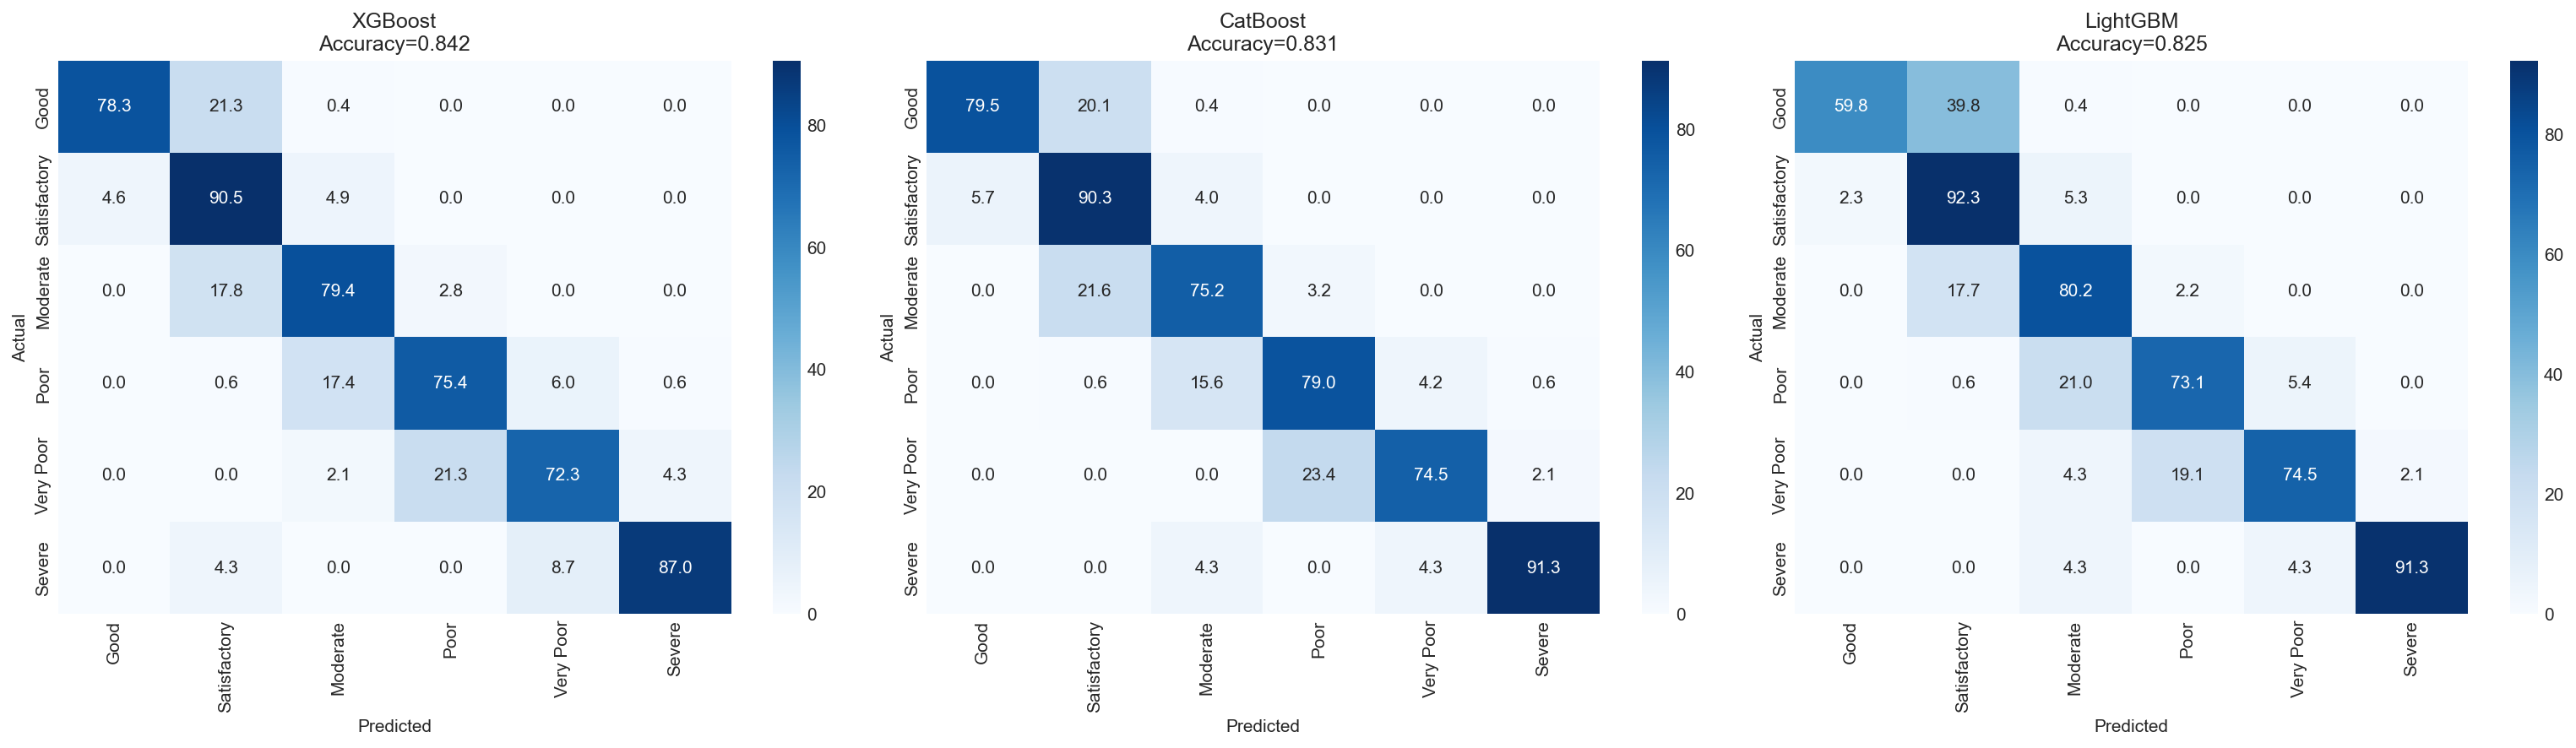
\includegraphics[width=\columnwidth]{figures/20_confusion_matrices.png}
\caption{Normalised confusion matrices for the top three classifiers. Misclassifications are concentrated between adjacent AQI categories (e.g., Satisfactory $\leftrightarrow$ Moderate, Poor $\leftrightarrow$ Very Poor), consistent with the ordinal nature of the target variable.}
\label{fig:confmat}
\end{figure}

Confusion matrix analysis (Fig.~\ref{fig:confmat}) confirms that misclassifications are almost exclusively between adjacent categories, which is expected given the ordinal nature of the AQI scale: the boundary between Satisfactory (AQI 100) and Moderate (AQI 101) is a single-unit threshold in a noisy, continuous measurement.

\subsection{Deep Learning Results}

\begin{table}[!t]
\centering
\caption{Deep Learning Model Performance on Test Set}
\label{tab:deeplearning}
\begin{tabular}{lcccc}
\toprule
\textbf{Architecture} & \textbf{$R^2$} & \textbf{RMSE} & \textbf{MAE} & \textbf{Epochs} \\
\midrule
Stacked LSTM       & 0.6732 & 39.93 & 19.92 & 32 \\
Conv1D-LSTM        & 0.6629 & 40.55 & 20.61 & 27 \\
Vanilla LSTM       & 0.6560 & 40.97 & 19.29 & 54 \\
Bidirectional LSTM & 0.6373 & 42.07 & 19.66 & 28 \\
GRU                & 0.6342 & 42.24 & 20.31 & 41 \\
\bottomrule
\end{tabular}
\end{table}

\begin{figure}[!t]
\centering
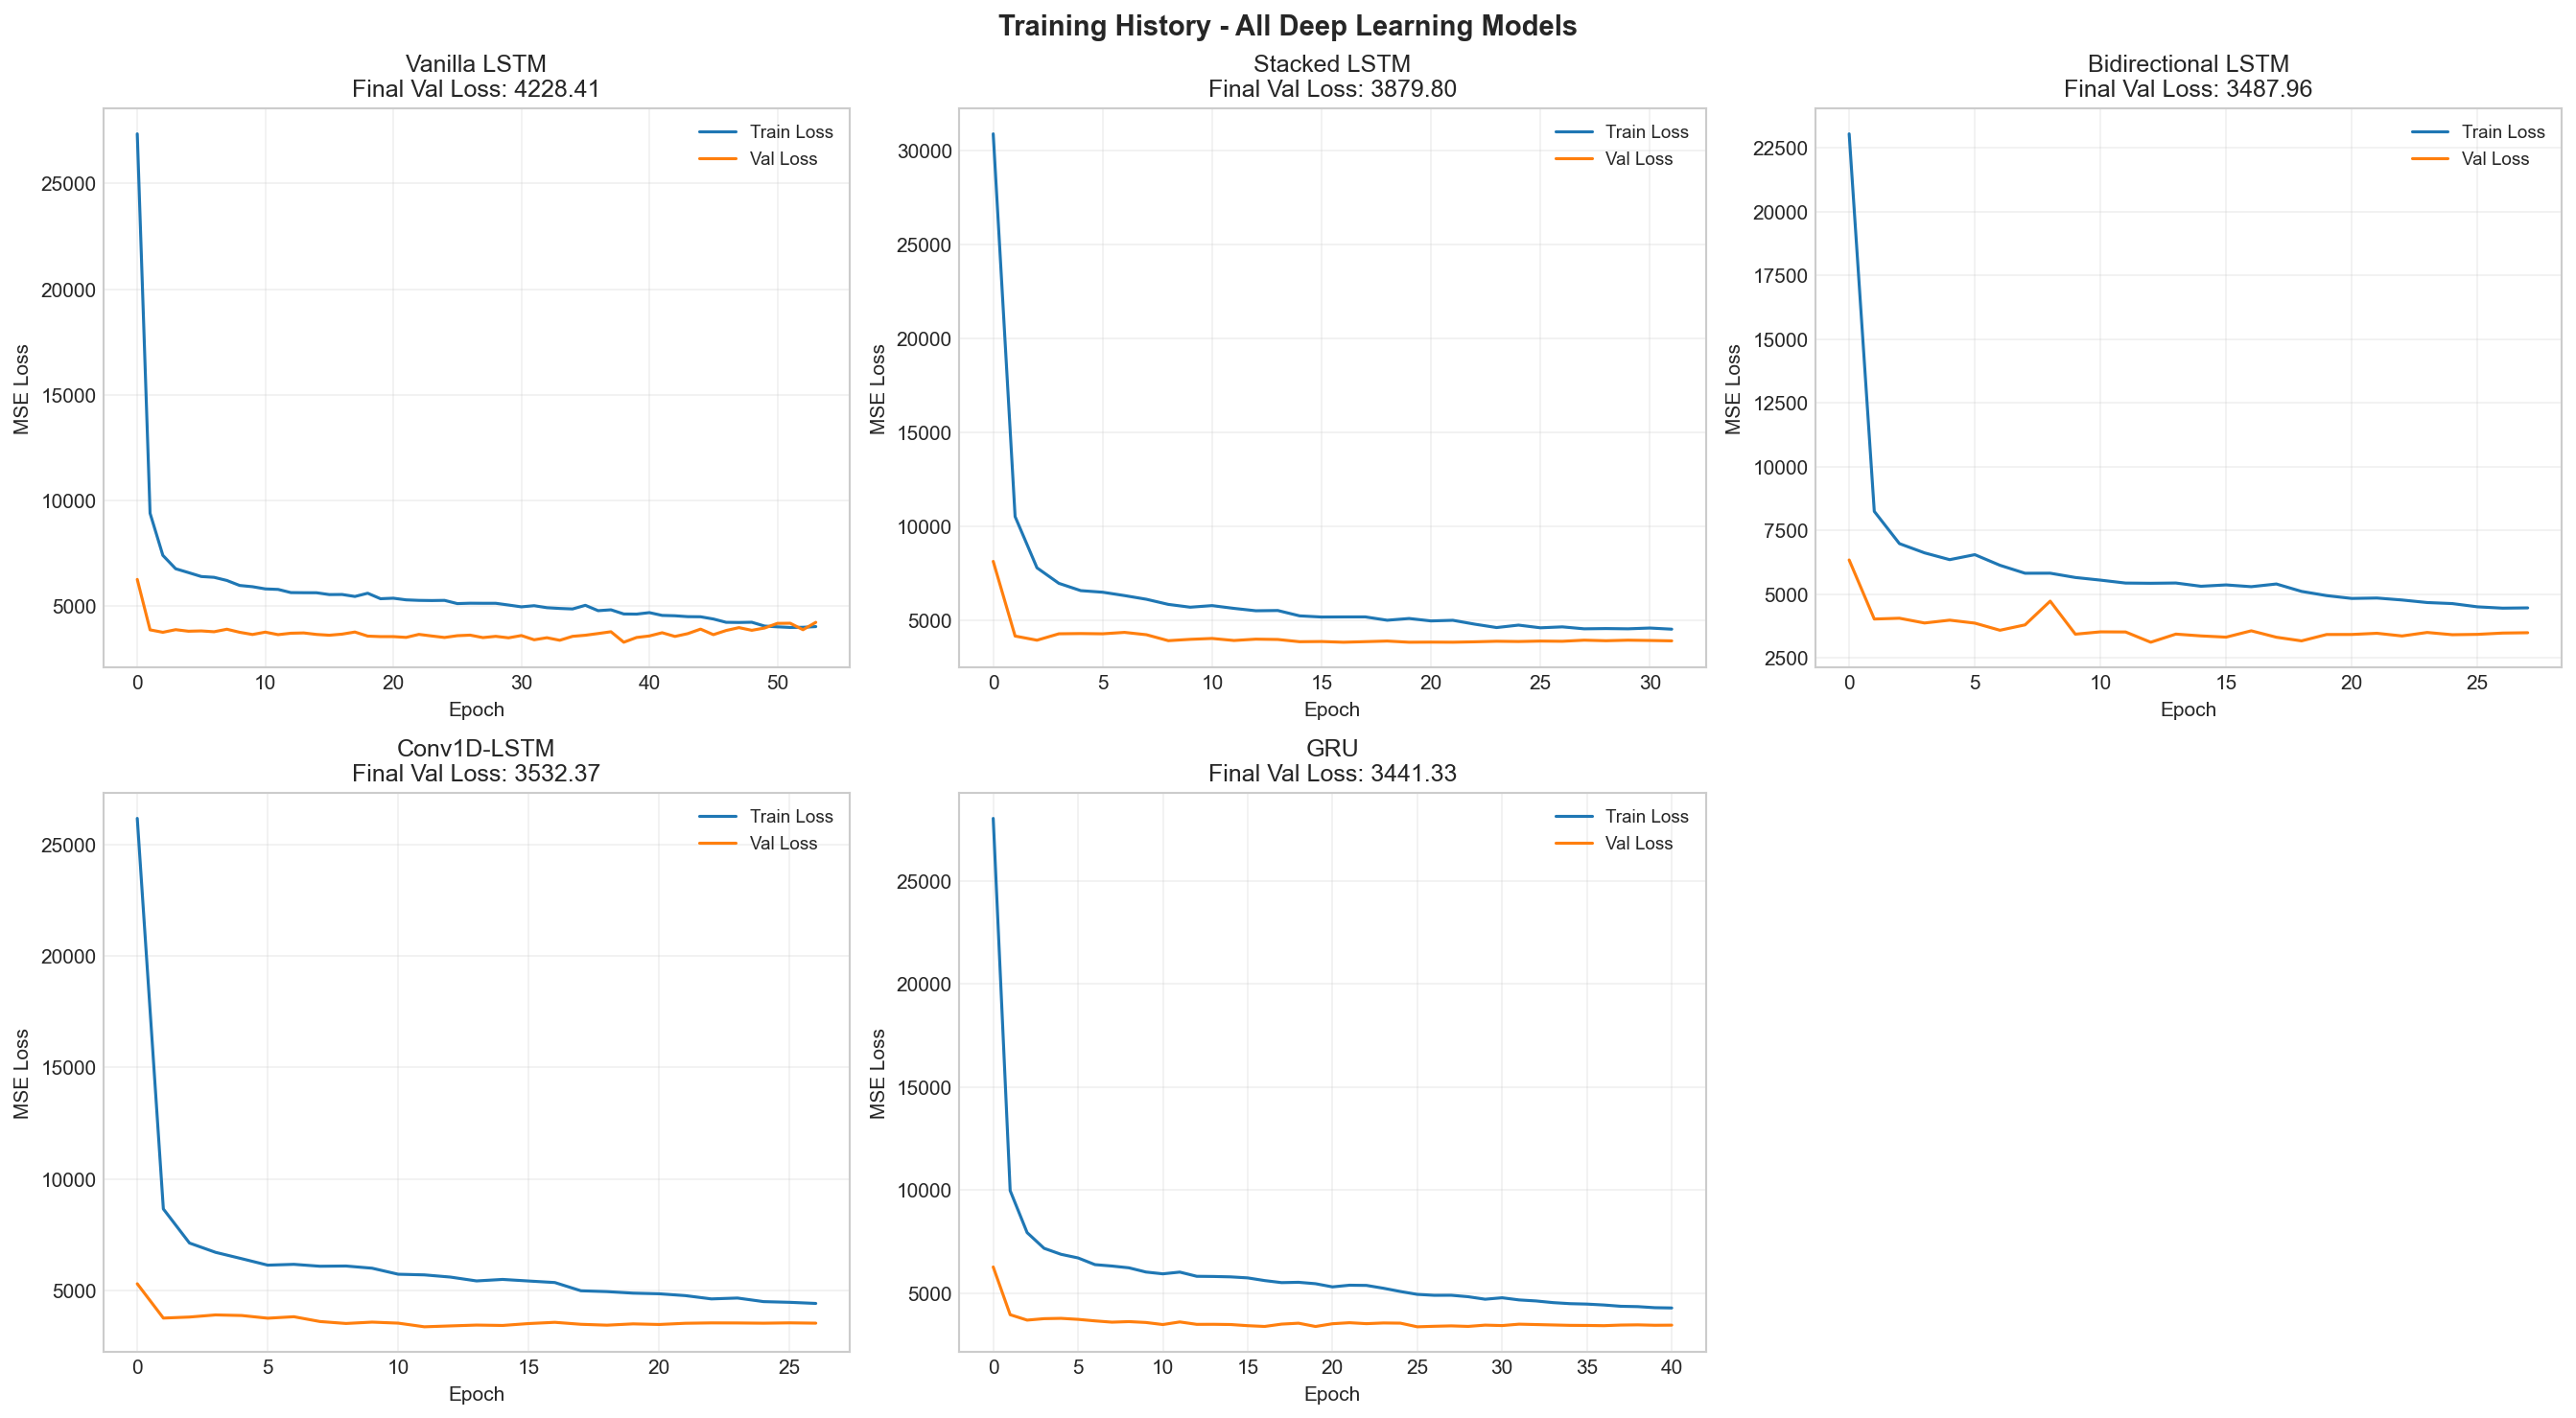
\includegraphics[width=\columnwidth]{figures/22_dl_training_history.png}
\caption{Training and validation loss curves for all five deep learning architectures. All models converge within 30--55 epochs with early stopping, but the final validation loss remains substantially higher than that achieved by gradient boosting methods.}
\label{fig:dlhistory}
\end{figure}

Table~\ref{tab:deeplearning} presents the deep learning results. The Stacked LSTM achieved the highest $R^2$ of 0.6732 with RMSE of 39.93, followed by Conv1D-LSTM ($R^2 = 0.6629$). All five architectures converged within 27--54 epochs (Fig.~\ref{fig:dlhistory}), but the best deep learning $R^2$ (0.673) underperforms LightGBM (0.901) by 22.8 percentage points.

\begin{figure}[!t]
\centering
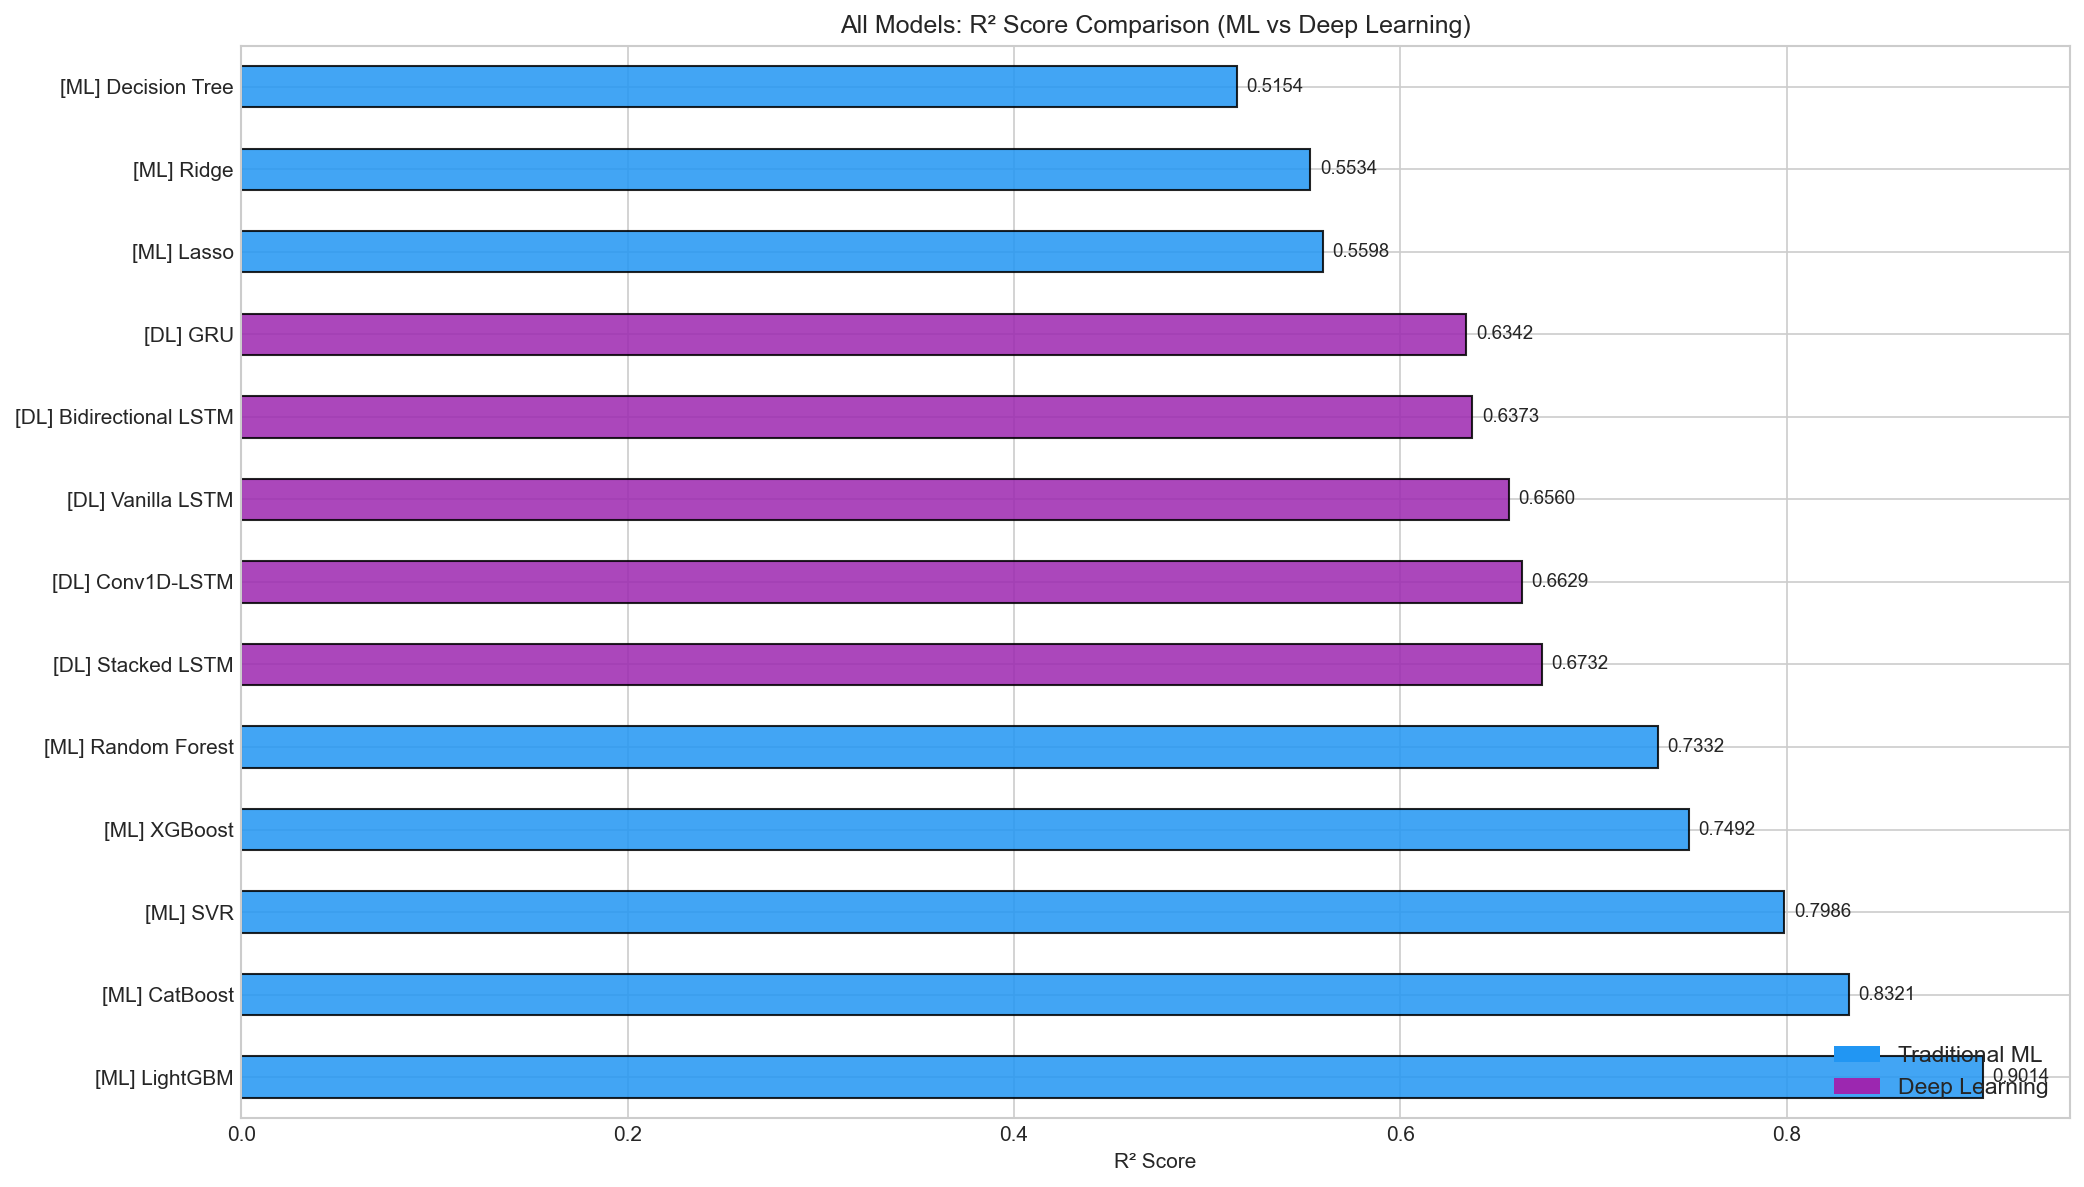
\includegraphics[width=\columnwidth]{figures/24_all_models_comparison.png}
\caption{Unified comparison of all 13 regression and deep learning models ranked by $R^2$. A performance plateau is evident within the gradient boosting family ($R^2 \approx 0.75$--$0.90$), with deep learning models clustered at $R^2 \approx 0.63$--$0.67$ and linear models at $R^2 \approx 0.55$.}
\label{fig:allmodels}
\end{figure}

The unified comparison (Fig.~\ref{fig:allmodels}) reveals a clear three-tier hierarchy: gradient boosting ($R^2 = 0.75$--$0.90$) $>$ deep learning ($R^2 = 0.63$--$0.67$) $>$ linear methods ($R^2 \approx 0.55$). This ordering corroborates the findings of Grinsztajn \textit{et al.} \cite{grinsztajn2022} and Shwartz-Ziv and Armon \cite{shwartzziv2022}: on tabular datasets with moderate dimensionality (141 features) and sample sizes below 50{,}000, tree-based models exploit hand-engineered features more effectively than recurrent networks operating on raw sequences.

The performance disparity is attributable to two factors. First, the 72 lag features and 48 rolling statistics explicitly encode the temporal dependencies that LSTMs must learn implicitly from raw sequences of only 7 features over 14 timesteps---an information-theoretic disadvantage. Second, gradient boosting inherently performs feature selection through split-point optimisation, whereas the dense layers in LSTM architectures assign non-zero weights to all input dimensions, including noisy or irrelevant pollutants.

\subsection{Hyperparameter Tuning Results}

\begin{table}[!t]
\centering
\caption{Optuna-Tuned Regression Model Performance}
\label{tab:optuna}
\begin{tabular}{lcccc}
\toprule
\textbf{Model} & \textbf{$R^2$} & \textbf{RMSE} & \textbf{MAE} & \textbf{$\Delta R^2$} \\
\midrule
\textbf{LightGBM (tuned)} & \textbf{0.9065} & \textbf{23.17} & \textbf{12.49} & +0.0051 \\
CatBoost (tuned)           & 0.8576 & 28.60 & 15.35 & +0.0255 \\
XGBoost (tuned)            & 0.7823 & 35.36 & 15.90 & +0.0331 \\
\bottomrule
\end{tabular}
\end{table}

\begin{figure}[!t]
\centering
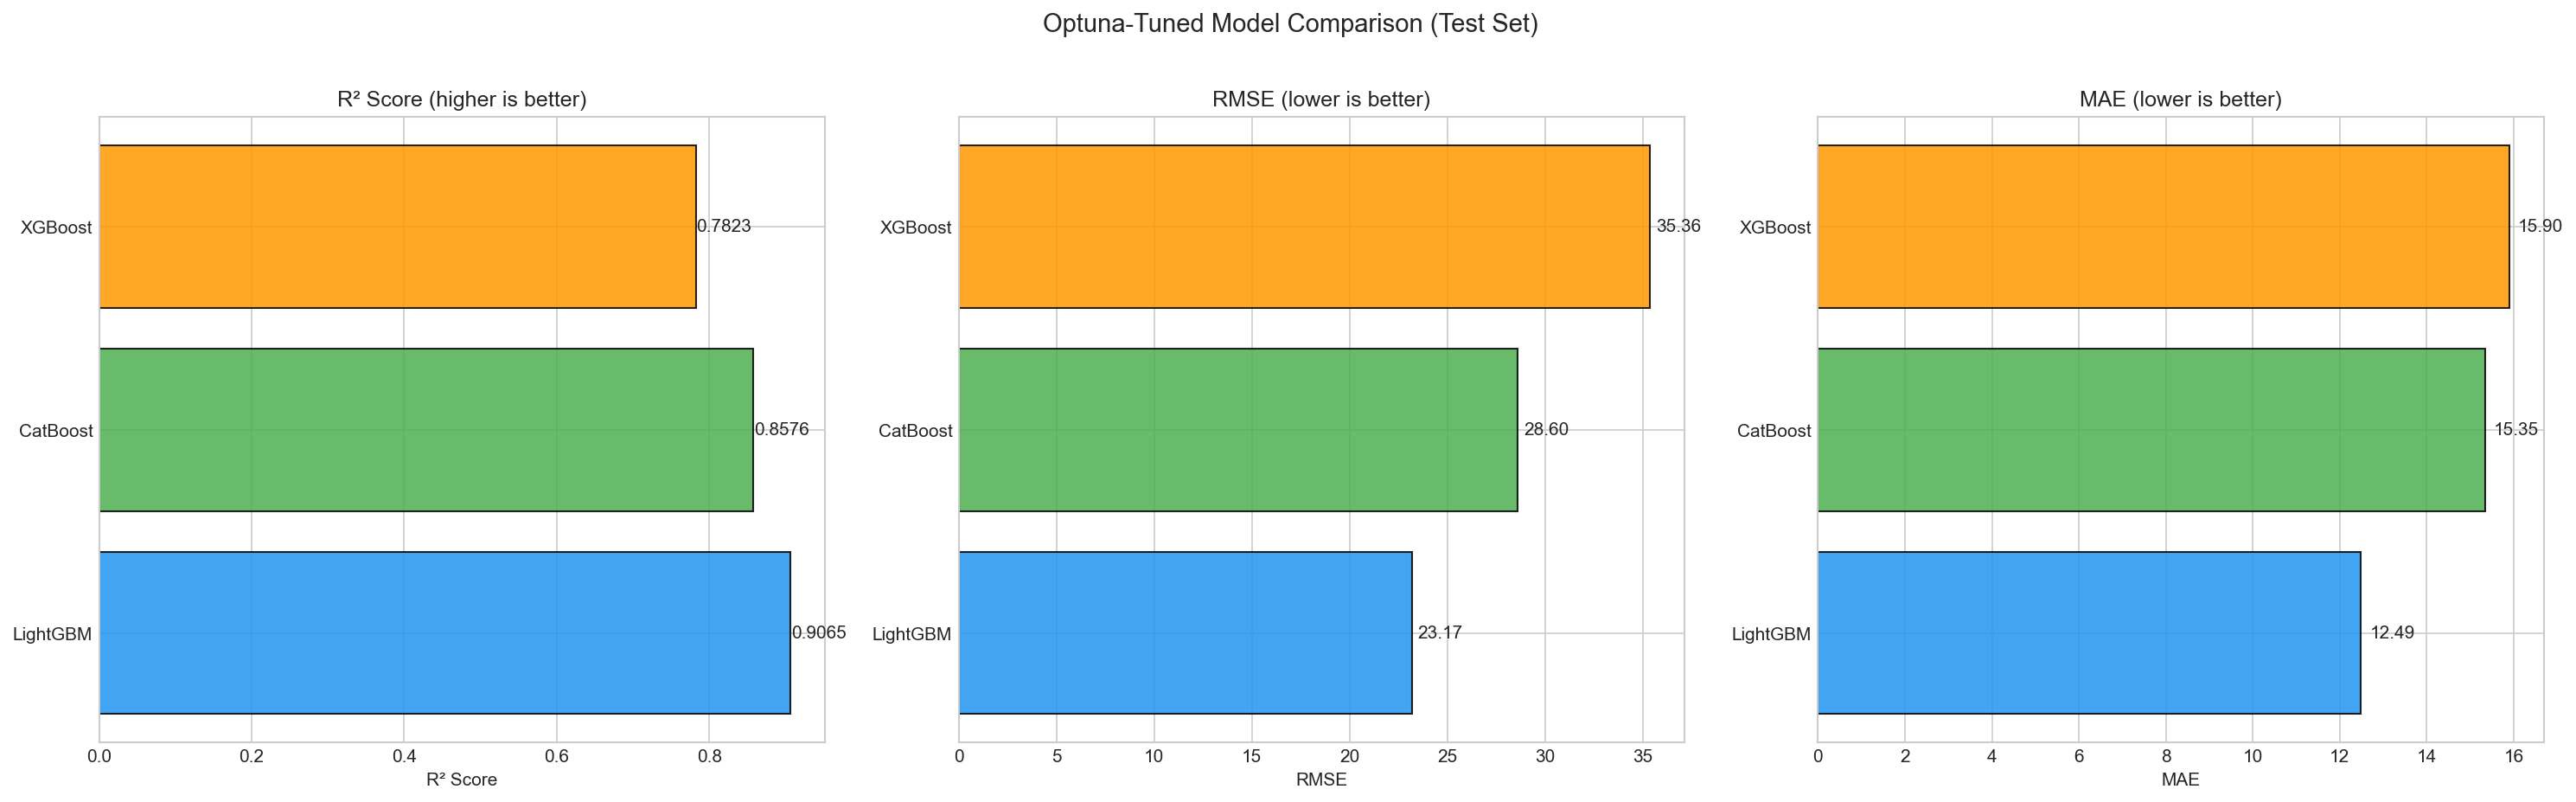
\includegraphics[width=\columnwidth]{figures/25_optuna_comparison.png}
\caption{Baseline versus Optuna-tuned performance for the top three regression models. LightGBM's improvement is marginal ($\Delta R^2 = 0.005$), while XGBoost benefits most from tuning ($\Delta R^2 = 0.033$), suggesting that LightGBM's default hyperparameters are already near-optimal for this dataset.}
\label{fig:optuna}
\end{figure}

Table~\ref{tab:optuna} and Fig.~\ref{fig:optuna} present the results after 50 Optuna trials per model. The tuned LightGBM achieved $R^2 = 0.9065$ (RMSE = 23.17), a modest $\Delta R^2 = +0.005$ improvement over its default configuration. CatBoost and XGBoost benefited more substantially from tuning ($\Delta R^2 = +0.026$ and $+0.033$, respectively), narrowing the gap to LightGBM but not closing it. The small marginal gain for LightGBM indicates that modern gradient boosting libraries ship with well-calibrated default hyperparameters, and the primary determinant of performance on this dataset is the quality of feature engineering rather than hyperparameter selection.

% ============================================================
% VI. EXPLAINABILITY ANALYSIS
% ============================================================
\section{Explainability Analysis}

\subsection{Global Feature Importance}

\begin{figure}[!t]
\centering
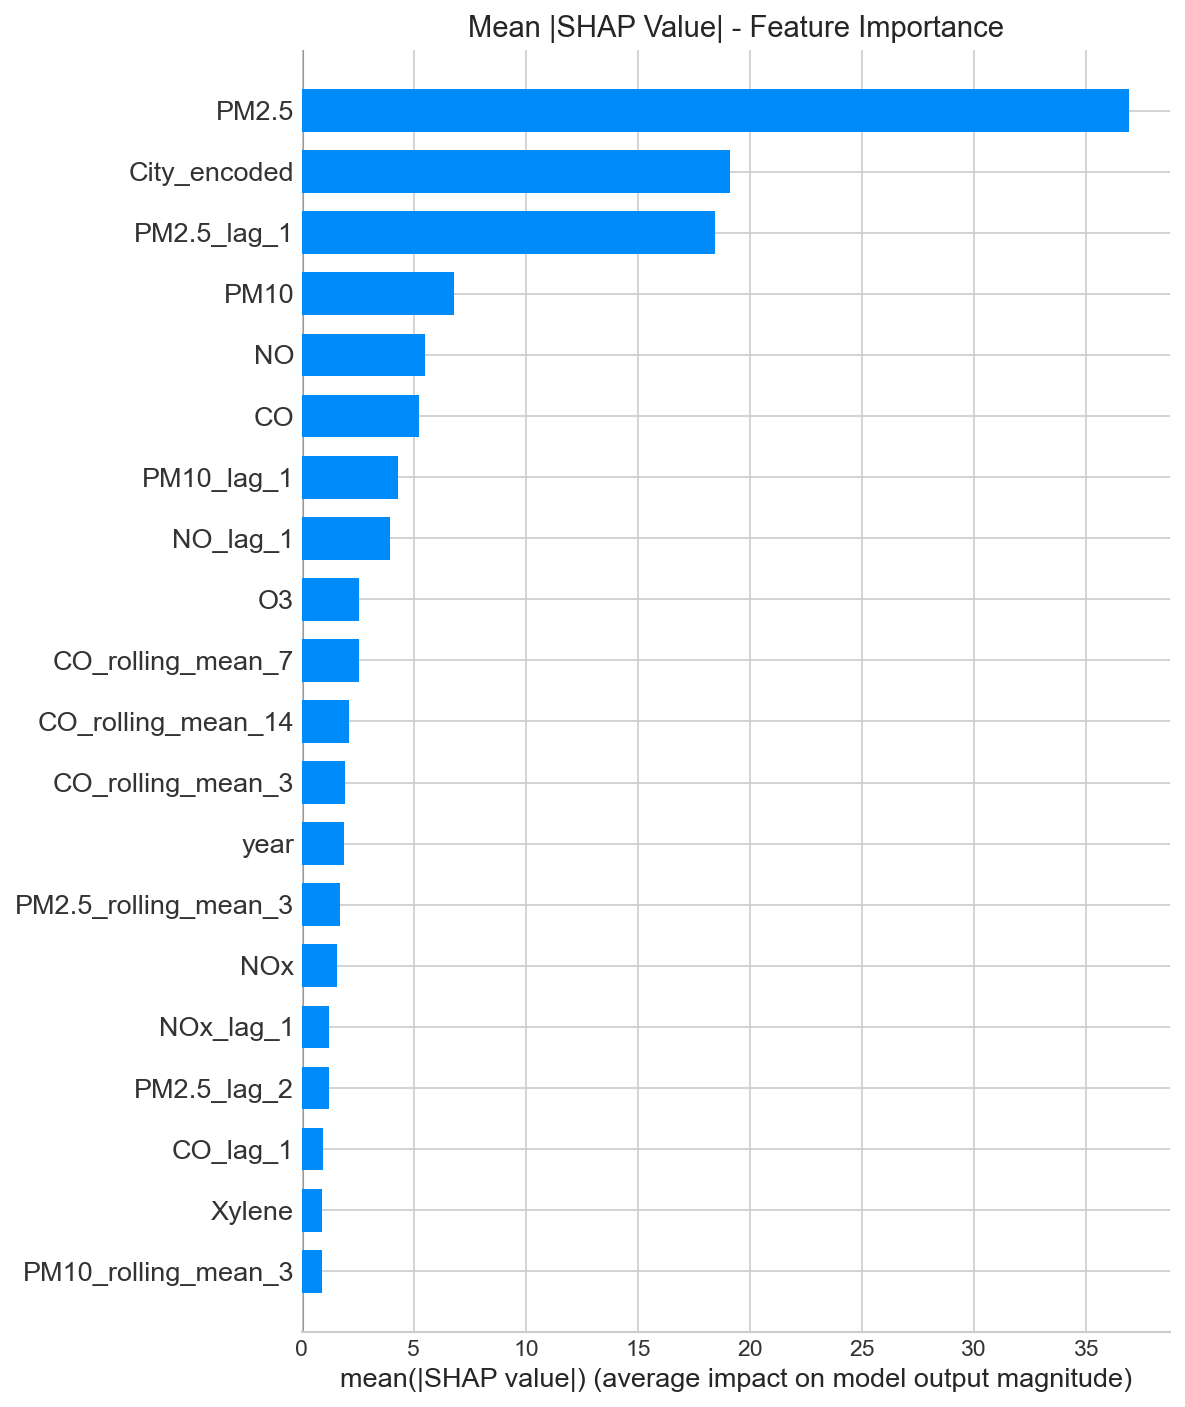
\includegraphics[width=\columnwidth]{figures/27_shap_bar.png}
\caption{Global feature importance via mean absolute SHAP values for the Optuna-tuned LightGBM model (500 test samples). PM\textsubscript{2.5} lag and rolling features dominate, followed by CO-related features and seasonal indicators.}
\label{fig:shapbar}
\end{figure}

Fig.~\ref{fig:shapbar} ranks features by mean $|\text{SHAP}|$ across 500 test observations. PM\textsubscript{2.5}-derived features (1-day lag, 7-day rolling mean, 3-day rolling mean) occupy the top positions, collectively accounting for the largest share of model output variation. CO rolling statistics appear prominently, consistent with CO's role as a tracer of combustion emissions---both vehicular and biomass-derived. Month and season features rank within the top 10, reflecting the strong seasonal modulation of Indian air quality. The city encoding feature also ranks highly, capturing baseline inter-city differences in pollution levels (e.g., Delhi's mean AQI of 235 versus Shillong's 44).

\subsection{Feature Interaction Analysis}

\begin{figure}[!t]
\centering
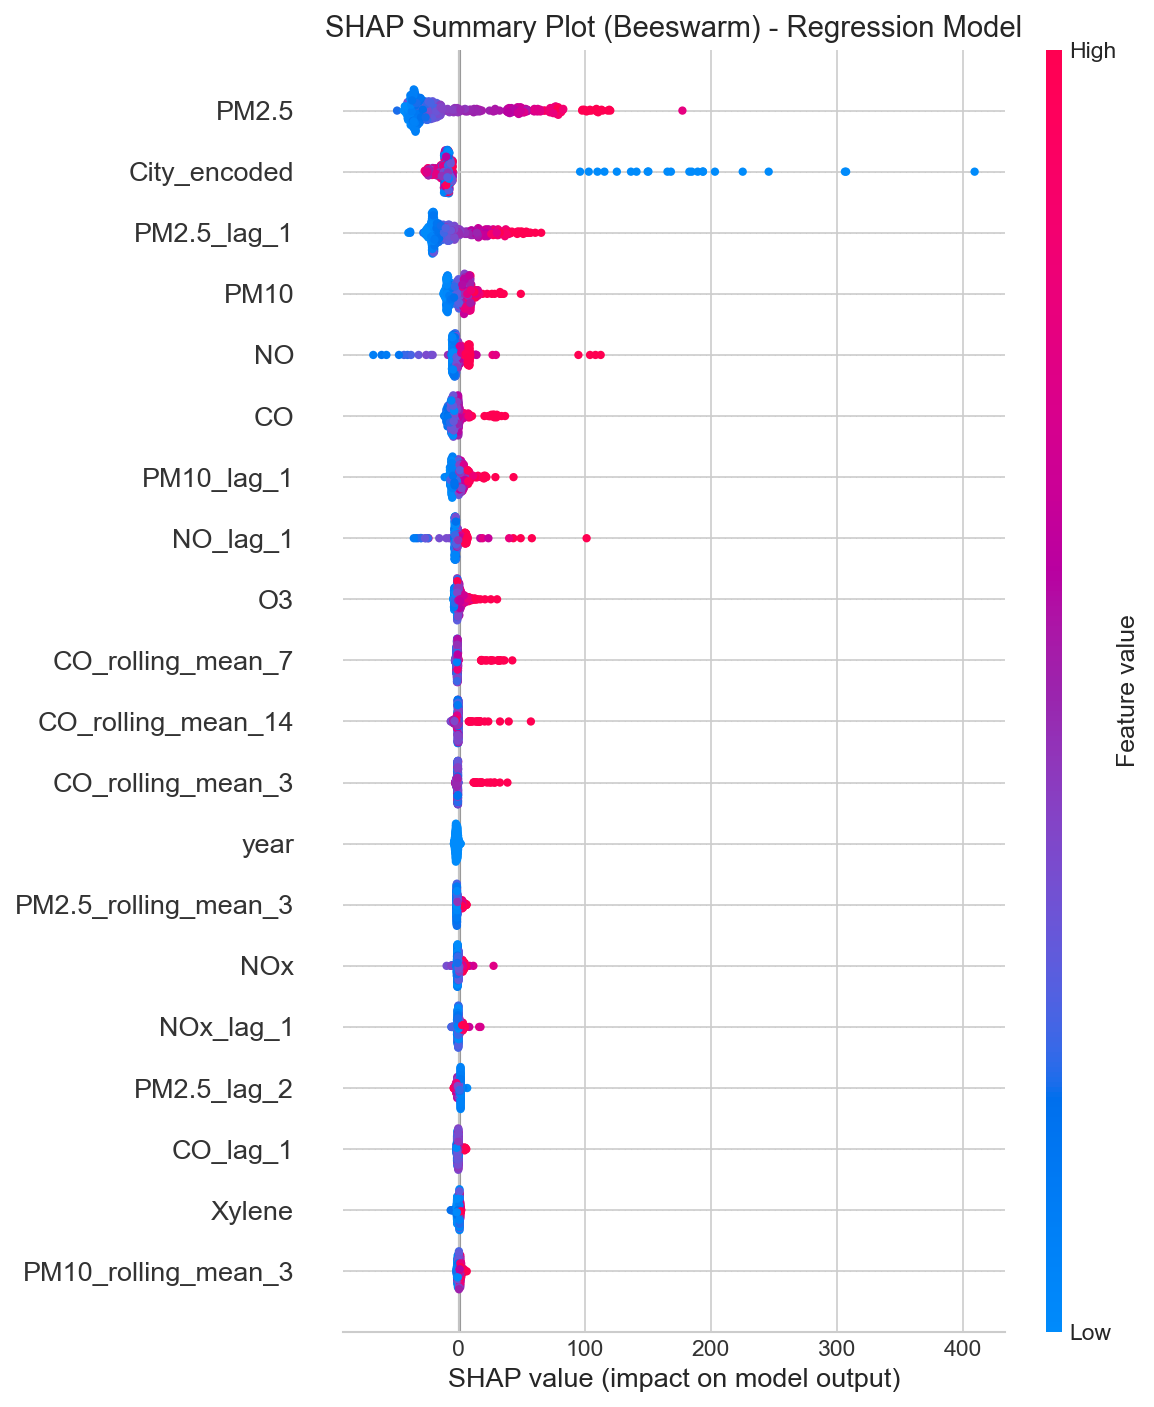
\includegraphics[width=\columnwidth]{figures/26_shap_summary.png}
\caption{SHAP beeswarm plot showing per-instance feature contributions. Each point represents one observation; colour encodes the feature's standardised value (red = high, blue = low). High PM\textsubscript{2.5} values (red) push SHAP values strongly positive (higher predicted AQI), while monsoon-season indicators (blue month values) push predictions negative.}
\label{fig:shapbeeswarm}
\end{figure}

The beeswarm plot (Fig.~\ref{fig:shapbeeswarm}) reveals clear directional relationships. For PM\textsubscript{2.5} lag features, high raw values (red points) consistently produce positive SHAP contributions, pushing the predicted AQI upward. The relationship is monotonic and approximately linear at low-to-moderate concentrations but exhibits diminishing marginal impact at extreme values, consistent with the CPCB sub-index breakpoint structure where the AQI-per-$\mu$g/m$^3$ slope decreases at higher concentration brackets.

The month feature displays a bimodal SHAP distribution: winter months (November--February, encoded as high values for month 11--12 and low values for month 1--2) produce positive SHAP contributions, while monsoon months (June--September) generate the strongest negative contributions. This pattern validates that the model has internalised India's seasonal pollution cycle rather than relying on spurious temporal correlations.

\subsection{Non-linear Effects and Feature Interactions}

\begin{figure}[!t]
\centering
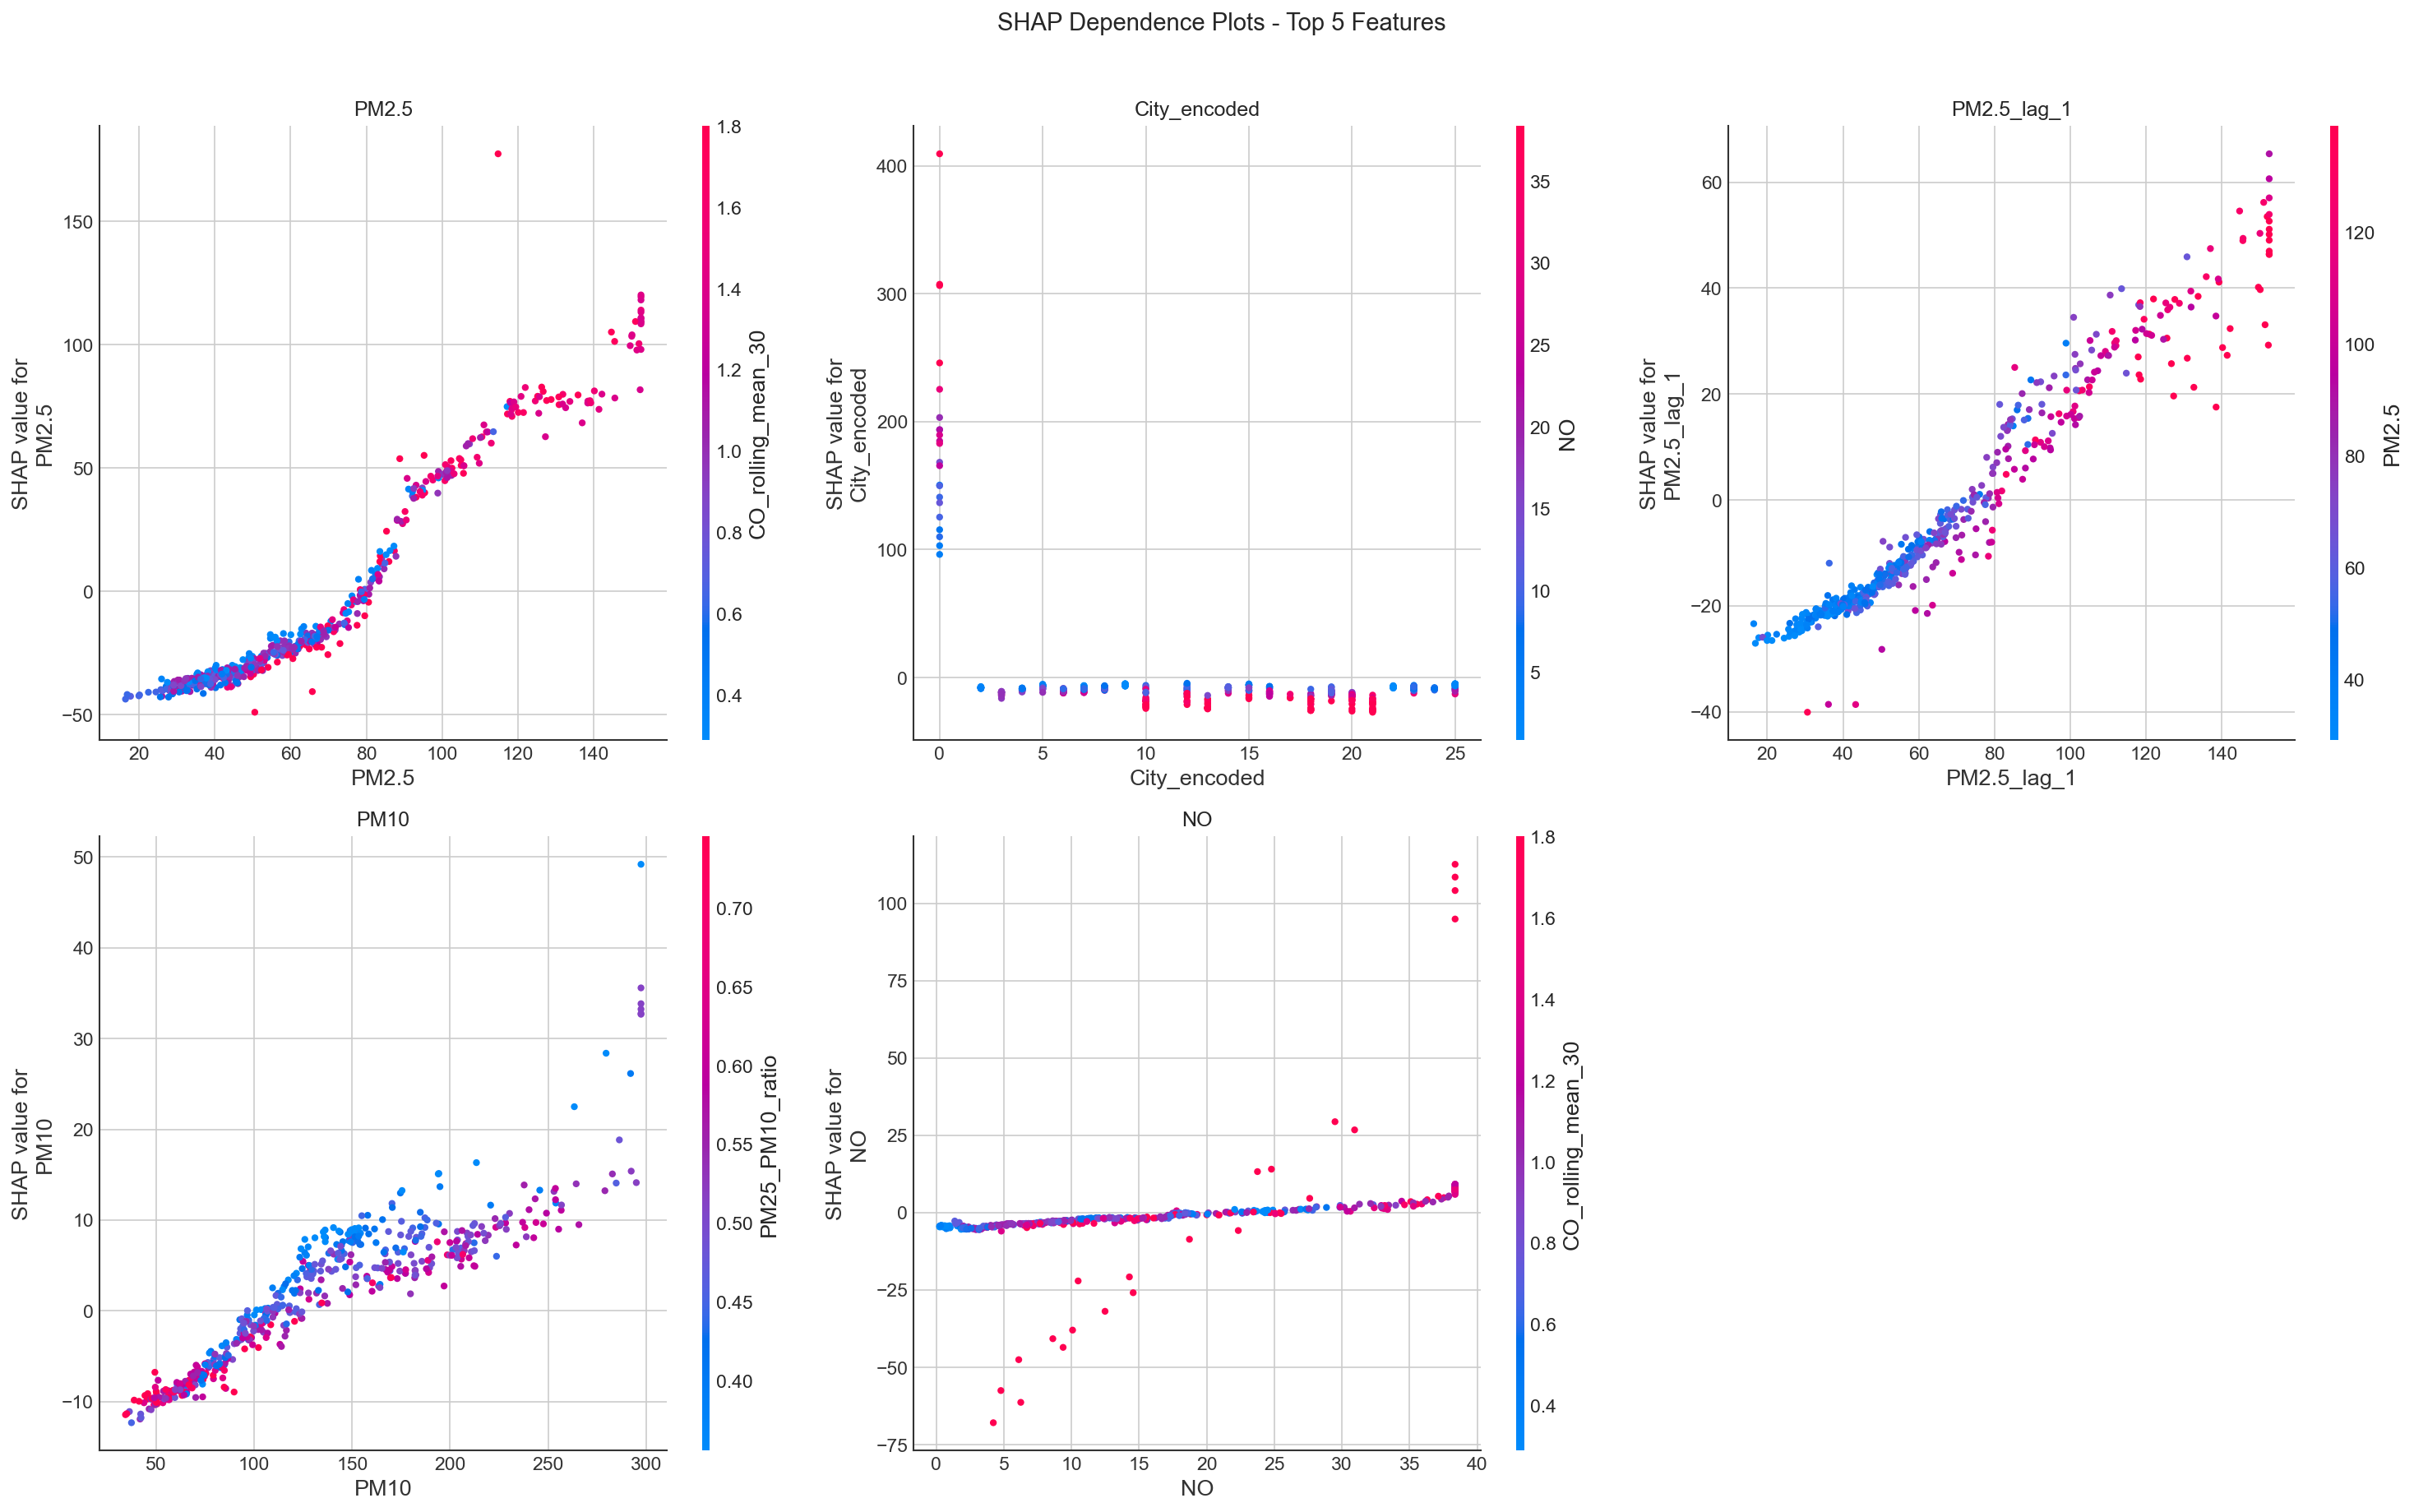
\includegraphics[width=\columnwidth]{figures/28_shap_dependence.png}
\caption{SHAP dependence plots for the top five features, with interaction colouring. PM\textsubscript{2.5} shows a monotonically increasing but saturating effect, while the month feature exhibits a V-shaped pattern with a minimum during the monsoon (July--August) and maxima during winter.}
\label{fig:shapdep}
\end{figure}

Dependence plots (Fig.~\ref{fig:shapdep}) expose non-linear feature--response relationships:

\textit{PM\textsubscript{2.5} 1-day lag.} The SHAP value increases monotonically with lagged PM\textsubscript{2.5} concentration but exhibits a slight saturation effect above 250~$\mu$g/m$^3$. Interaction colouring reveals that co-elevation of PM\textsubscript{10} (red points clustered in the upper-right region) amplifies the positive SHAP contribution, indicating a synergistic effect when both fine and coarse particulate matter are simultaneously elevated---characteristic of combined vehicular emissions and construction dust events.

\textit{CO rolling mean.} CO SHAP values are near-zero below 1.0~mg/m$^3$ and increase steeply above 2.0~mg/m$^3$, consistent with CO's threshold-like behaviour: low-level CO indicates clean conditions, while elevated CO signals proximity to combustion sources.

\textit{Month.} A V-shaped SHAP pattern is observed, with a minimum in July--August (monsoon washout) and maximum in November--December (post-monsoon crop burning and onset of winter inversions). The transition is not symmetric: the October--November increase is sharper than the March--April decrease, reflecting the abrupt onset of stubble burning versus the gradual improvement during spring.

\subsection{Classification SHAP Analysis}

\begin{figure}[!t]
\centering
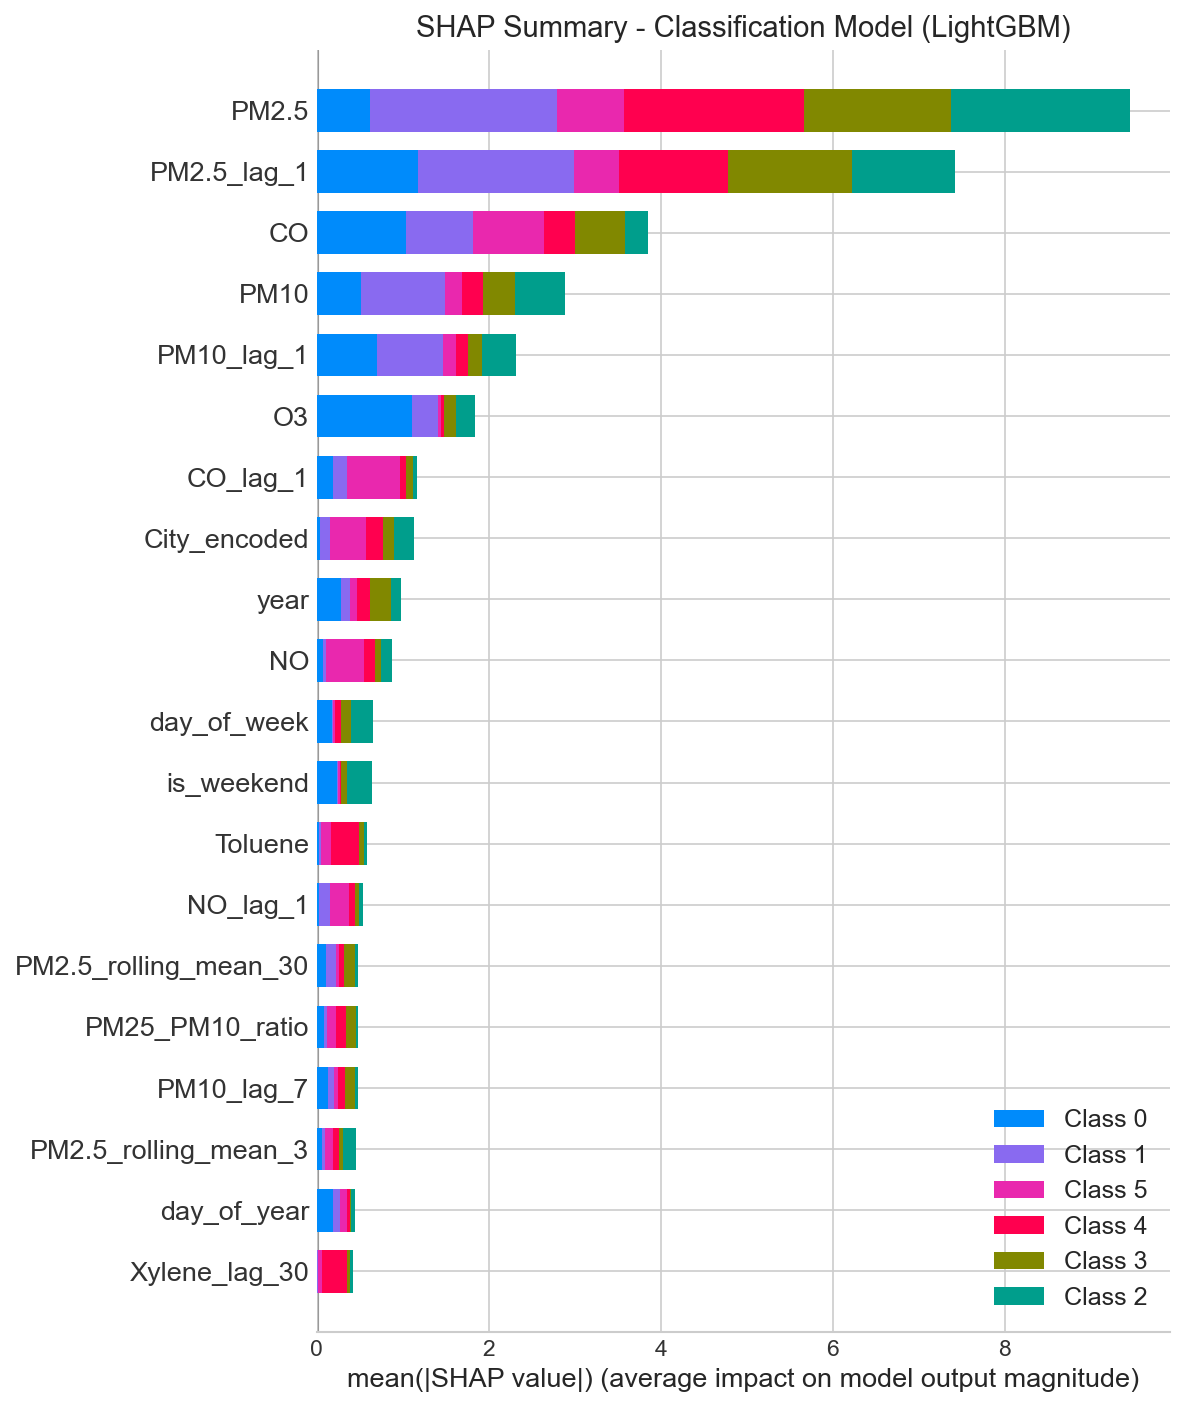
\includegraphics[width=\columnwidth]{figures/29_shap_classification.png}
\caption{SHAP analysis for the XGBoost classifier, stratified by AQI category. Feature importance profiles differ markedly across categories: PM\textsubscript{2.5} lag features dominate Severe/Very Poor predictions, while seasonal and city features play a larger role in Good/Satisfactory classifications.}
\label{fig:shapclass}
\end{figure}

Per-class SHAP analysis for the XGBoost classifier (Fig.~\ref{fig:shapclass}) reveals category-specific feature profiles. For Severe and Very Poor predictions, PM\textsubscript{2.5} and CO lag features produce SHAP values 3--5$\times$ larger than for lower-severity categories, indicating that extreme pollution events are driven almost entirely by particulate and combustion-marker concentrations. In contrast, Good and Satisfactory predictions rely more heavily on seasonal features and city encoding: monsoon season combined with a coastal or northeastern city shifts the prediction toward low-AQI categories even when some individual pollutant readings are moderately elevated. This class-stratified analysis demonstrates that the model has learned distinct decision pathways for benign versus hazardous air quality conditions, rather than applying a single threshold-based rule.

\subsection{Validation Against Domain Knowledge}

The SHAP-derived feature importance hierarchy is consistent with established atmospheric science and the CPCB AQI methodology:

\begin{enumerate}
    \item \textbf{PM\textsubscript{2.5} dominance}: PM\textsubscript{2.5} is the dominant sub-index pollutant in approximately 60--70\% of CPCB AQI computations. Its prominence in SHAP rankings confirms that the model has learned the actual AQI determination mechanism.
    \item \textbf{Seasonal patterns}: The winter maximum / monsoon minimum in SHAP values mirrors the well-documented seasonal cycle of Indian air quality, driven by boundary layer dynamics, precipitation patterns, and emission source variation \cite{guttikunda2013}.
    \item \textbf{CO as combustion tracer}: The prominence of CO features aligns with its role as a marker for incomplete combustion---from vehicular traffic, biomass cooking, and crop residue burning \cite{ganguly2020}.
    \item \textbf{City-level variation}: The high SHAP importance of the city feature reflects genuine geographic heterogeneity: landlocked basin cities (Delhi, Patna) have fundamentally different pollutant dispersion characteristics compared to coastal (Mumbai, Kochi) or elevated (Shillong) locations.
\end{enumerate}

% ============================================================
% VII. DISCUSSION
% ============================================================
\section{Discussion}

\subsection{Key Findings and Implications}

Six principal findings emerge from this study. First, gradient boosting models---particularly LightGBM---outperform all other paradigms on this structured tabular dataset, achieving an $R^2$ of 0.9065 with training times under 10 seconds, making them suitable for operational deployment. Second, feature engineering is the primary determinant of predictive performance: the 72 lag features and 48 rolling statistics that encode temporal persistence account for the majority of the $R^2$ gap between tree-based models ($\sim$0.90) and deep learning models ($\sim$0.67) that operate on raw sequences. Third, seasonal and temporal features capture India-specific pollution dynamics---winter inversions, monsoon washout, post-monsoon crop burning---that are difficult for models to learn from pollutant concentrations alone. Fourth, SMOTE oversampling outperforms built-in class weighting for multi-class AQI classification, improving accuracy by 2.7 percentage points. Fifth, Bayesian hyperparameter tuning via Optuna provides diminishing returns for LightGBM ($\Delta R^2 = 0.005$), suggesting that default configurations are already near-optimal for well-engineered features. Sixth, SHAP analysis validates that learned model behaviour aligns with atmospheric science, establishing a basis for trust in model-generated predictions.

\subsection{COVID-19 as a Natural Experiment}

\begin{figure}[!t]
\centering
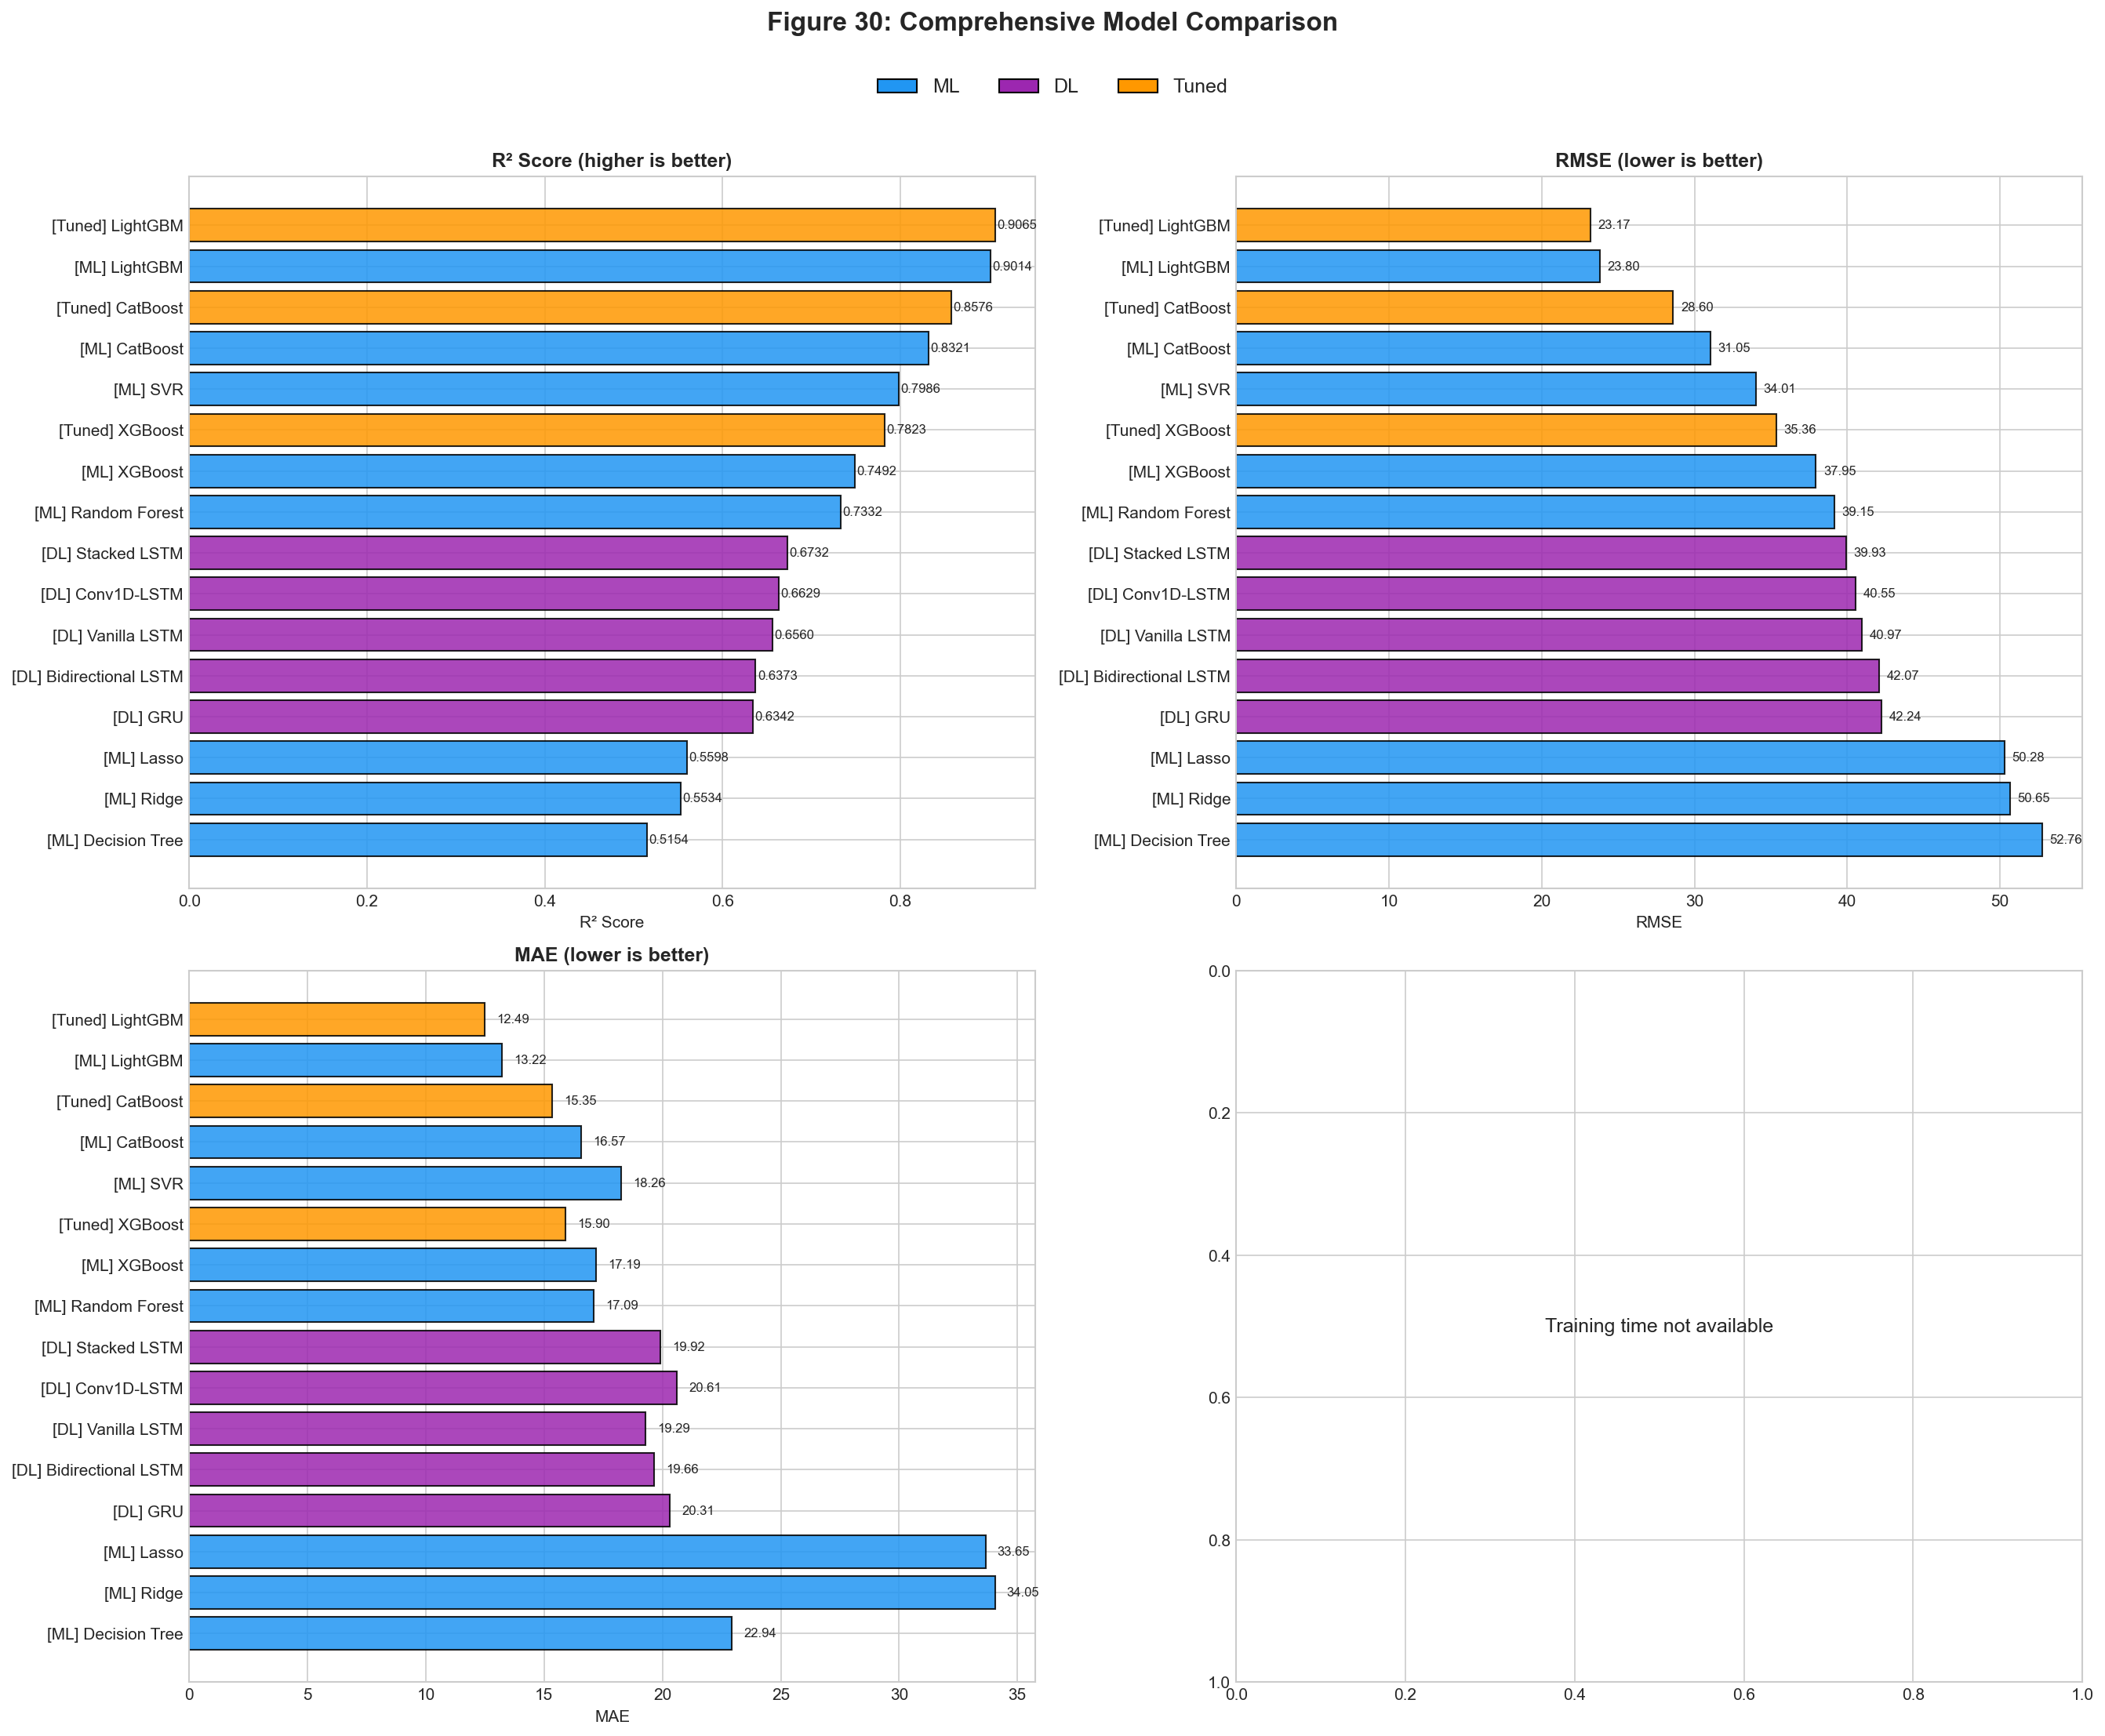
\includegraphics[width=\columnwidth]{figures/30_final_comparison.png}
\caption{Final comparison of selected production models across regression and classification paradigms, including the selected LightGBM (regression) and XGBoost (classification) models deployed in the operational application.}
\label{fig:final}
\end{figure}

The test set (February--July 2020) encompasses an extreme distributional shift: India's national lockdown reduced vehicular traffic by 70--90\% and industrial output by 40--60\% \cite{mahato2020, sharmaetal2020}, producing AQI readings 30--50\% below historical norms for the corresponding calendar period. The LightGBM model's $R^2$ of 0.9065 on this test set demonstrates that it has captured genuine pollutant--AQI relationships rather than memorising year-over-year temporal patterns. Had the model relied on temporal memorisation, the unprecedented lockdown-era AQI values would have produced systematic overprediction---an effect not observed in the residual analysis (Fig.~\ref{fig:residuals}).

This finding has implications beyond model validation: it suggests that the learned feature--AQI mappings can be used to estimate the air quality impact of hypothetical policy interventions (e.g., vehicular restrictions, industrial shutdowns) by adjusting the pollutant concentration inputs, with the model providing an empirically grounded response surface.

\subsection{Limitations}

Several limitations should be acknowledged. First, the feature set is confined to pollutant concentrations and temporal indicators; meteorological variables (wind speed, humidity, temperature, boundary layer height) and external factors (satellite-derived aerosol optical depth, traffic density) are not included, which may limit predictive performance in transitional weather conditions. Second, the city is treated as a categorical variable with no spatial modelling of inter-city pollutant transport (e.g., smoke plume advection from Punjab to Delhi). Third, the dataset operates at daily granularity; hourly predictions would require different architectural choices and face greater noise. Fourth, SHAP values were computed on 500 test samples for computational tractability; while this is sufficient for stable global importance rankings, individual explanations may vary with larger samples. Fifth, the study uses a single data source (CPCB); external validation on independent monitoring networks (e.g., US Embassy PM\textsubscript{2.5} monitors) would strengthen generalisability claims.

\subsection{Comparison with Prior Work}

The achieved $R^2$ of 0.9065 for regression compares favourably with published results on Indian AQI data. Kumar and Pande \cite{kumar2022} reported $R^2$ values of 0.78--0.85 using random forests and gradient boosting on a smaller five-city subset, without feature engineering or hyperparameter tuning. The 84.16\% classification accuracy exceeds the 72--79\% range reported by Masood and Ahmad \cite{masood2023} in their review of AQI classification studies. Direct comparison is complicated by differences in dataset scope, preprocessing, and evaluation methodology; however, the breadth of the current comparison (20 models, 3 paradigms, SHAP analysis) substantially exceeds that of any prior Indian AQI study.

% ============================================================
% VIII. CONCLUSION AND FUTURE WORK
% ============================================================
\section{Conclusion and Future Work}

This paper presented a systematic evaluation of 20 machine learning models across regression, classification, and deep learning paradigms for Air Quality Index prediction in India. The Optuna-tuned LightGBM regressor achieved $R^2 = 0.9065$ (RMSE = 23.17 AQI units) on 24{,}850 daily observations from 26 cities (2015--2020), while an XGBoost classifier attained 84.16\% accuracy across six CPCB-defined severity categories after SMOTE-based class balancing. Five deep learning architectures (LSTM variants and GRU) substantially underperformed gradient boosting methods ($R^2 \leq 0.673$), corroborating recent benchmarks that tree-based models retain a decisive advantage on structured tabular data.

A 141-feature engineering pipeline---incorporating temporal lags, rolling statistics, pollutant ratios, and seasonal encodings---was identified as the primary driver of predictive performance. SHAP explainability analysis confirmed that the dominant predictive features (PM\textsubscript{2.5} lags, seasonal indicators, CO rolling statistics) are consistent with the atmospheric science of Indian air quality, establishing a principled basis for model trust. The test set's coverage of India's 2020 COVID-19 lockdown provided a natural experiment demonstrating that the models have learned genuine pollutant--AQI relationships robust to extreme distributional shift.

Future work should pursue several directions. Incorporation of meteorological variables (wind speed and direction, temperature, humidity, mixing layer height) from reanalysis products or station observations is expected to improve performance in transitional weather conditions. Spatial modelling using graph neural networks, with cities as nodes and transport corridors as edges, could capture inter-city pollutant advection. Extension to hourly granularity would support real-time health advisory systems, though this requires fundamentally different sequence modelling approaches. Transfer learning from data-rich cities (Delhi, Mumbai) to data-sparse stations could address the monitoring infrastructure gap. Finally, integration of satellite-derived PM\textsubscript{2.5} estimates (e.g., from NASA's MERRA-2 or Copernicus CAMS) would provide spatial continuity beyond the 26 CPCB cities.

A prototype real-time prediction system based on the findings of this study has been deployed as a Streamlit web application, ingesting live pollutant data from the World Air Quality Index (WAQI) API and generating 7-day AQI forecasts with causal analysis and health advisories for 26 Indian cities.

% ============================================================
% REFERENCES
% ============================================================
\begin{thebibliography}{34}

\bibitem{who2021}
World Health Organization, ``WHO Global Air Quality Guidelines: Particulate Matter (PM\textsubscript{2.5} and PM\textsubscript{10}), Ozone, Nitrogen Dioxide, Sulfur Dioxide and Carbon Monoxide,'' WHO, Geneva, 2021.

\bibitem{balakrishnan2019}
K.~Balakrishnan \textit{et al.}, ``The impact of air pollution on deaths, disease burden, and life expectancy across the states of India: the Global Burden of Disease Study 2017,'' \textit{The Lancet Planetary Health}, vol.~3, no.~1, pp.~e26--e39, 2019.

\bibitem{guttikunda2013}
S.~K. Guttikunda and R.~Calori, ``A GIS based emissions inventory at 1~km $\times$ 1~km spatial resolution for air pollution analysis in Delhi, India,'' \textit{Atmospheric Environment}, vol.~67, pp.~101--111, 2013.

\bibitem{cpcb2014}
Central Pollution Control Board (CPCB), ``National Air Quality Index,'' Ministry of Environment, Forest and Climate Change, Government of India, 2014.

\bibitem{kumar2022}
K.~Kumar and B.~P. Pande, ``Air pollution prediction with machine learning: a case study of Indian cities,'' \textit{International Journal of Environmental Science and Technology}, vol.~20, pp.~5333--5348, 2023.

\bibitem{sharma2020}
E.~Sharma, R.~Deo, R.~Prasad, and A.~V. Parisi, ``A hybrid air quality early-warning framework: an hourly forecasting model with online sequential extreme learning machines and empirical mode decomposition algorithms,'' \textit{Science of the Total Environment}, vol.~709, p.~135934, 2020.

\bibitem{masood2023}
A.~Masood and K.~Ahmad, ``A review on emerging artificial intelligence (AI) techniques for air pollution forecasting: fundamentals, application and performance,'' \textit{Journal of Cleaner Production}, vol.~322, p.~129072, 2021.

\bibitem{grinsztajn2022}
L.~Grinsztajn, E.~Oyallon, and G.~Varoquaux, ``Why do tree-based models still outperform deep learning on typical tabular data?,'' in \textit{Proc. NeurIPS 2022 Datasets and Benchmarks Track}, 2022.

\bibitem{mahato2020}
S.~Mahato, S.~Pal, and K.~G. Ghosh, ``Effect of lockdown amid COVID-19 pandemic on air quality of the megacity Delhi, India,'' \textit{Science of the Total Environment}, vol.~730, p.~139086, 2020.

\bibitem{chen2016}
T.~Chen and C.~Guestrin, ``XGBoost: A scalable tree boosting system,'' in \textit{Proc. 22nd ACM SIGKDD Int. Conf. Knowledge Discovery and Data Mining}, pp.~785--794, 2016.

\bibitem{ke2017}
G.~Ke \textit{et al.}, ``LightGBM: A highly efficient gradient boosting decision tree,'' in \textit{Advances in Neural Information Processing Systems}, vol.~30, pp.~3146--3154, 2017.

\bibitem{prokhorenkova2018}
L.~Prokhorenkova, G.~Gusev, A.~Vorobev, A.~V. Dorogush, and A.~Gulin, ``CatBoost: unbiased boosting with categorical features,'' in \textit{Advances in Neural Information Processing Systems}, vol.~31, 2018.

\bibitem{hochreiter1997}
S.~Hochreiter and J.~Schmidhuber, ``Long Short-Term Memory,'' \textit{Neural Computation}, vol.~9, no.~8, pp.~1735--1780, 1997.

\bibitem{cho2014}
K.~Cho \textit{et al.}, ``Learning phrase representations using RNN encoder-decoder for statistical machine translation,'' in \textit{Proc. EMNLP}, pp.~1724--1734, 2014.

\bibitem{breiman2001}
L.~Breiman, ``Random Forests,'' \textit{Machine Learning}, vol.~45, no.~1, pp.~5--32, 2001.

\bibitem{cortes1995}
C.~Cortes and V.~Vapnik, ``Support-vector networks,'' \textit{Machine Learning}, vol.~20, no.~3, pp.~273--297, 1995.

\bibitem{lundberg2017}
S.~M. Lundberg and S.-I. Lee, ``A unified approach to interpreting model predictions,'' in \textit{Advances in Neural Information Processing Systems}, vol.~30, pp.~4765--4774, 2017.

\bibitem{ribeiro2016}
M.~T. Ribeiro, S.~Singh, and C.~Guestrin, ```Why should I trust you?': Explaining the predictions of any classifier,'' in \textit{Proc. 22nd ACM SIGKDD}, pp.~1135--1144, 2016.

\bibitem{lundberg2020}
S.~M. Lundberg \textit{et al.}, ``From local explanations to global understanding with explainable AI for trees,'' \textit{Nature Machine Intelligence}, vol.~2, pp.~56--67, 2020.

\bibitem{molnar2022}
C.~Molnar, \textit{Interpretable Machine Learning: A Guide for Making Black Box Models Explainable}, 2nd~ed., 2022.

\bibitem{chawla2002}
N.~V. Chawla, K.~W. Bowyer, L.~O. Hall, and W.~P. Kegelmeyer, ``SMOTE: Synthetic Minority Over-sampling Technique,'' \textit{Journal of Artificial Intelligence Research}, vol.~16, pp.~321--357, 2002.

\bibitem{troyanskaya2001}
O.~Troyanskaya \textit{et al.}, ``Missing value estimation methods for DNA microarrays,'' \textit{Bioinformatics}, vol.~17, no.~6, pp.~520--525, 2001.

\bibitem{akiba2019}
T.~Akiba, S.~Sano, T.~Yanase, T.~Ohta, and M.~Koyama, ``Optuna: A next-generation hyperparameter optimization framework,'' in \textit{Proc. 25th ACM SIGKDD}, pp.~2623--2631, 2019.

\bibitem{shwartzziv2022}
R.~Shwartz-Ziv and A.~Armon, ``Tabular data: Deep learning is not all you need,'' \textit{Information Fusion}, vol.~81, pp.~84--90, 2022.

\bibitem{borisov2022}
V.~Borisov \textit{et al.}, ``Deep neural networks and tabular data: A survey,'' \textit{IEEE Transactions on Neural Networks and Learning Systems}, vol.~35, no.~6, pp.~7499--7519, 2024.

\bibitem{li2020}
X.~Li, L.~Peng, X.~Yao, S.~Cui, Y.~Hu, C.~You, and T.~Chi, ``Long short-term memory neural network for air pollutant concentration predictions: method development and evaluation,'' \textit{Environmental Pollution}, vol.~231, pp.~997--1004, 2017.

\bibitem{pak2020}
U.~Pak, J.~Ma, U.~Ryu, K.~Ryom, U.~Juhyok, K.~Pak, and C.~Pak, ``Deep learning-based PM2.5 prediction considering the spatiotemporal correlations: a case study of Beijing, China,'' \textit{Science of the Total Environment}, vol.~699, p.~134279, 2020.

\bibitem{castelli2020}
M.~Castelli, F.~M. Clemente, A.~Popovic, S.~Silva, and L.~Vanneschi, ``A machine learning approach to predict air quality in California,'' \textit{Complexity}, vol.~2020, p.~8049504, 2020.

\bibitem{soh2018}
P.~W. Soh, J.~W. Chang, and J.~N. Huang, ``Adaptive deep learning-based air quality prediction model using the most relevant spatial-temporal relations,'' \textit{IEEE Access}, vol.~6, pp.~58186--58199, 2018.

\bibitem{sharmaetal2020}
S.~Sharma, M.~Zhang, Anshika, J.~Gao, H.~Zhang, and S.~H. Kota, ``Effect of restricted emissions during COVID-19 on air quality in India,'' \textit{Science of the Total Environment}, vol.~728, p.~138878, 2020.

\bibitem{berman2020}
J.~D. Berman and K.~Ebisu, ``Changes in US air quality during the COVID-19 pandemic,'' \textit{Science of the Total Environment}, vol.~739, p.~139864, 2020.

\bibitem{ganguly2020}
T.~Ganguly \textit{et al.}, ``National Clean Air Programme (NCAP) for Indian Cities: Review and outlook of clean air action plans,'' \textit{Atmospheric Environment: X}, vol.~8, p.~100096, 2020.

\bibitem{hastie2009}
T.~Hastie, R.~Tibshirani, and J.~Friedman, \textit{The Elements of Statistical Learning}, 2nd~ed., Springer, 2009.

\bibitem{ncap2019}
Ministry of Environment, Forest and Climate Change, ``National Clean Air Programme (NCAP),'' Government of India, 2019.

\end{thebibliography}

\end{document}
